\chapter{Results}
\label{sec:results}

This chapter contains results from testing six different models on four test datasets. The six models consists of three SSD models and three Yolo models trained on different data. This produces a significant amount of results, and it makes the task of presenting the results in an orderly fashion challenging. To try to overcome this challenge this chapter is structured in the following way:

\begin{enumerate}
    \item Present datasets and models. Explain abbreviations used later in the chapter.
    \item Overview of results.
    \item Present case studies of more interesting aspects of results.
\end{enumerate}

\noindent
The case studies  and test datasets were chosen to shed some light on the following questions.

\begin{itemize}
    \item How does training on a building class affect the performance on detection of boats
    \item How does training on boats in coast near environments affect detection accuracy in open sea
    \item How does SSD compare to Yolo when trained and tested on the same data
    \item In which situations do the detection algorithms struggle, and in which situations is the performance satisfactory
\end{itemize}

In this chapter, datasets are mentioned when referring both to training and testing of models. All the custom datasets are split into test and training subsets, which are used respectively for testing and training.

\section{Terminology and Abbreviations}
Yolo and SSD were trained on three different combinations of datasets:


\begin{enumerate}
    \item Trondheimsfjorden, boats\_far, boats\_close
    \item Trondheimsfjorden, boats\_far, boats\_close, boats\_buildings\_buildings\_not\_labelled
    \item Trondheimsfjorden, boats\_far, boats\_close, boats\_buidings, buildings
\end{enumerate}

\vspace{3mm}
\noindent
The following abbreviations will be used for the datasets. 

\begin{table}[h!]
\begin{tabular}{l|l|l}
Abbreviation & Explanation                                      & Datasets                                  \\ \hline
bh           & {[}B{]}oats {[}H{]}ouses                         & boats\_buildings                          \\
bhnl         & {[}B{]}oats {[}H{]}ouses {[}N{]}ot {[}L{]}abeled & boats\_buildings\_buildings\_not\_labeled \\
bc           & {[}B{]}oats {[}C{]}lose                          & boats\_close                              \\
bf           & {[}B{]}oats {[}F{]}ar                            & boats\_far                                \\
build        & Buildings                                        & buildings                                 \\
trf          & Trondheimsfjorden                                & trondheimsfjorden                        
\end{tabular}
\end{table}

The \textit{bhnl} dataset contains the same images as the \textit{bh} dataset, the difference is that the buildings in \textit{bhnl} are not labeled. The letter "h" have been used as an abbreviation for buildings (houses) to differentiate it from "b" which is used for boats.

\vspace{3mm}

Henceforth the model names in table \ref{tab_models} will be used to distinguish the models trained on different data.

\begin{table}[h!]
\centering
\begin{tabular}{l|ll}
Model name  & Trained on datasets    & Description                        \\ \hline
Yolo1, SSD1 & \textit{trf}, \textit{bc}, \textit{bf}            & Boats sailing                           \\
Yolo2, SSD2 & \textit{trf}, \textit{bc}, \textit{bf}, \textit{bhnl}      & Boats sailing, boats moored            \\
Yolo3, SSD3 & \textit{trf}, \textit{bc}, \textit{bf}, \textit{bh}, \textit{build} & Boats sailing, boats moored, buildings
\end{tabular}
\caption{Model description}
\label{tab_models}
\end{table}

\vspace{3mm}

The model number signifies which data, and how much data, the model has been trained on. The higher the model number, the higher the amount of training data.


\section{Results Overview}

To present an overview of the results two statistics have been used. The first one is a table of the average precision (AP) of each model on four test datasets. The second is confusion matrices. Both average precision and confusion matrices are explained in chapter \ref{sec:eval}. Chapter \ref{subsec:ap} presents the average precision results, chapter \ref{subsec:cm} presents the confusion matrices, chapter \ref{subsec:main} discusses the most important aspects of these results.

\newpage

\subsection{Average Precision}
\label{subsec:ap}

The average precision of the models on the different test datasets is shown in table \ref{ap_tab}. The average precision gives a good indication of how well the detection model perform on a dataset, and gives a more complete picture than confusion matrices.

\begin{table}[h!]
\centering
\begin{tabular}{l|ll|ll|ll}
Tested on   & Yolo1 & SSD1  & Yolo2 & SSD2  & Yolo3 & SSD3  \\ \hline
\textit{bhnl}        & 0.182 & 0.140 & 0.707 & 0.515 & 0.701 & 0.586 \\
\textit{trf}         & 0.885 & 0.860 & 0.900 & 0.750 & 0.908 & 0.876 \\
\textit{bc}, \textit{bf}      & 0.509 & 0.278 & 0.533 & 0.239 & 0.647 & 0.292 \\
\textit{bc}, \textit{bf}, \textit{trf} & 0.577 & 0.375 & 0.600 & 0.329 & 0.726 & 0.391
\end{tabular}
\caption{Average precisions}
\label{ap_tab}
\end{table}


\subsection{Confusion Matrices}
\label{subsec:cm}

As explained in chapter \ref{sec:conf_mat}, confusion matrices gives an intuitive understanding of the results. In this chapter two tables are presented, in the tables each model's confusion matrix on the four datasets are presented. The difference between the two tables are the confidence threshold set for the detection. The bounding boxes Yolo and SSD outputs comes with a confidence score, indicating how confident the algorithm is in the detection. A higher confidence threshold would lead to fewer false positives, but possibly also fewer true positives, the confidence thresholds used for the two tables presented here are 0.25 and 0.5. The confusion matrices are presented as shown in table \ref{tab:conf_exp}.



% Please add the following required packages to your document preamble:
% \usepackage{multirow}
\begin{table}[h!]
\centering
\begin{tabular}{c|ll}
\multicolumn{1}{l|}{}  & \multicolumn{2}{l}{Dataset (Number of objects in dataset)} \\ \hline
\multirow{2}{*}{Model} & True positives        & False positives                    \\
                       & False negatives       & True negatives (Not relevant)     
\end{tabular}
\caption{Confusion matrix explanation}
\label{tab:conf_exp}
\end{table}

% Please add the following required packages to your document preamble:
% \usepackage{multirow}
\begin{table}[h!]
\centering
\begin{tabular}{l|ll|ll|ll|ll}
                       & \multicolumn{2}{l|}{BB (58)} & \multicolumn{2}{l|}{TRF (174)} & \multicolumn{2}{l|}{BcBf (818)} & \multicolumn{2}{l}{BcBfTrf (992)} \\ \hline
\multirow{2}{*}{Yolo1} & 13            & 21           & 164            & 22            & 551            & 435            & 715              & 457             \\
                       & 45            &              & 10             &               & 267            &                & 277              &                 \\ \hline

\multirow{2}{*}{Yolo2} & 39            & 4            & 167            & 8             & 555            & 263            & 722              & 271             \\
                       & 19            &              & 7              &               & 263            &                & 270              &                 \\ \hline
\multirow{2}{*}{Yolo3} & 40            & 6            & 173            & 3             & 611            & 214            & 784              & 217             \\
                       & 18            &              & 1              &               & 207            &                & 208              &                 \\ \hline
\multirow{2}{*}{SSD1}  & 7             & 15           & 151            & 17            & 359            & 315            & 510              & 332             \\
                       & 51            &              & 23             &               & 459            &                & 482              &                 \\ \hline
\multirow{2}{*}{SSD2}  & 32            & 20           & 146            & 34            & 323            & 437            & 469              & 471             \\
                       & 26            &              & 28             &               & 495            &                & 523              &                 \\ \hline

\multirow{2}{*}{SSD3}  & 32            & 13           & 150            & 23            & 365            & 282            & 515              & 305             \\
                       & 26            &              & 24             &               & 453            &                & 477              &                
\end{tabular}
\caption{Confusion matrix with the confidence threshold set to 0.25}
\label{tab:conf_025}
\end{table}


% Please add the following required packages to your document preamble:
% \usepackage{multirow}
\begin{table}[h!]
\centering
\begin{tabular}{l|ll|ll|ll|ll}
                       & \multicolumn{2}{l|}{BB (58)} & \multicolumn{2}{l|}{TRF (174)} & \multicolumn{2}{l|}{BcBf (818)} & \multicolumn{2}{l|}{BcBfTrf (992)} \\ \hline
\multirow{2}{*}{Yolo1} & 11            & 10           & 160            & 15            & 524            & 311            & 684              & 326             \\
                       & 47            &              & 14             &               & 294            &                & 308              &                 \\ \hline
\multirow{2}{*}{Yolo2} & 35            & 1            & 165            & 6             & 498            & 198            & 663              & 204             \\
                       & 23            &              & 9              &               & 320            &                & 329              &                 \\ \hline
\multirow{2}{*}{Yolo3} & 36            & 4            & 170            & 2             & 577            & 149            & 747              & 151             \\
                       & 22            &              & 4              &               & 241            &                & 245              &                 \\ \hline
\multirow{2}{*}{SSD1}  & 6             & 11           & 142            & 11            & 333            & 251            & 475              & 262             \\
                       & 52            &              & 32             &               & 485            &                & 517              &                 \\ \hline
\multirow{2}{*}{SSD2}  & 29            & 9            & 136            & 22            & 299            & 338            & 435              & 360             \\
                       & 29            &              & 38             &               & 519            &                & 557              &                 \\ \hline
\multirow{2}{*}{SSD3}  & 31            & 6            & 147            & 14            & 319            & 214            & 466              & 228             \\
                       & 27            &              & 27             &               & 499            &                & 526              &                
\end{tabular}
\caption{Confusion matrix with the confidence threshold set to 0.5}
\label{tab:conf_05}
\end{table}

\vspace{3mm}


\subsection{Main results}
\label{subsec:main}

\subsubsection{Yolo3}
Yolo3 has the best overall results. On the \textit{trf} dataset Yolo3 has an average precision of 0.908, which is impressive. Table \ref{tab:conf_025}, where the confidence threshold is set to 0.25, shows that Yolo3 detects 173 out of 174 boats in this dataset, with only three false positives. When the confidence threshold is set to 0.5, Yolo3 detects 170 out of 174 boats, with two false positives, as shown in table \ref{tab:conf_05}. Even though the results on the other datasets are worse than on the \textit{trf} dataset, they are not bad. In \citep{YOLOv3}, Yolo gets a mean average precision, which is AP for multi-class detection, of 0.553 on the COCO dataset. To compare the average precision on the custom datasets to the results on the multi-class detection problem on the COCO dataset is not a fair comparison, but it still is worth noting to give a better intuition for what the average precisions shown in table \ref{ap_tab} means. 

\subsubsection{Effect of training differences}
The hypothesis before running the tests in this work was that more relevant training data used in a model, the better the test results. This means that the expected results was that Yolo3 would be better than Yolo2 which again would be better than Yolo1, and the same for the SSD models. While Yolo3 and SSD3 is better their MODELS??,  Yolo2 and SSD2 are outperformed by Yolo1 and SSD1 in most cases. This means that training on the \textit{build} dataset has a big effect on the test results on all datasets. This will be further discussed in chapter \ref{case_study:eff_build}.  YOLO2 HAR BEDRE AP, IKKE BEDRE PÅ CONFUSION MATRIX.

\subsubsection{Yolo vs. SSD}
As shown in the tables in chapter \ref{subsec:ap} and \ref{subsec:cm}, Yolo performs better than SSD in this project. One of the critical differences between Yolo and SSD was discussed in chapter \ref{sec:obj_det}, where SSD uses grids at multiple scales to detect objects, while Yolo only applies one. The hypothesis was that this would make SSD better at identifying boats that varied more in size, while Yolo would only detect boats within a certain size range. This hypothesis was not confirmed during the work on this project. Yolo detects more boats and has fewer misclassifications than SSD in all the tests done in this work.

\vspace{3mm}

In this project SSD mobilenet was used, a lightweight version of SSD meant for real-time solutions. SSD Mobilenet is faster, but less accurate compared to the original implementation. The reason for choosing Mobilenet over the original implementation was that it was used in a project at DNV GL the summer of 2018 with promising results. While Yolo and the original implementation of SSD has comparable accuracy, the accuracy of SSD Mobilenet is lower, meaning Yolo's superior accuracy is not entirely unexpected. 




\vspace{1cm}

BC BF not taken from a boat
Angle on image








\newpage

\section{Case Study 1: Effect from training on buildings}
\label{case_study:eff_build}

Both \citep{Tangstad2017} and \citep{Kamsvag2018} implemented an object detector for maritime vessels using Faster R-CNN. A challenge highlighted in both these projects was the misclassification of waterfront buildings as boats. To address this problem the datasets \textit{building\_boats} and \textit{buildings} were produced. By training the object detector on a building class, it may be able to detect the buildings as buildings and thus suppress the classifications of waterfront buildings as boats. As a first step in trying to verify this hypothesis, both Yolo and SSD were trained on two different sets of data. The two datasets they are trained on contains the same set of images with two exceptions:

\vspace{1mm}

\begin{enumerate}
    \item For Yolo2 and SSD2 only boats are labeled.
    \item For Yolo3 and SSD3 buildings are labeled in the dataset building\_boats, and a dataset containing only waterfront buildings was added to the training dataset.
\end{enumerate}

\vspace{1mm}

Thus, all the models have been trained on the same boat objects, while Yolo3 and SSD3 also have been trained on a building class. This has been done to try to minimize the variation in the variables that affect boat detection, and try to only look at how adding a building class affects the boat detection performance.

\vspace{3mm}

In figure \ref{fig:case_build} the precision/recall-curves for the models are displayed for the four test cases. For both SSD and Yolo the model trained on buildings generally performs better than Yolo2 and SSD2. However, the difference is more significant for SSD than for Yolo. How much training on a building class affects the results differ depending on which dataset was used for testing. 

\begin{figure}[h!]
\begin{subfigure}{.5\textwidth}
  \centering
  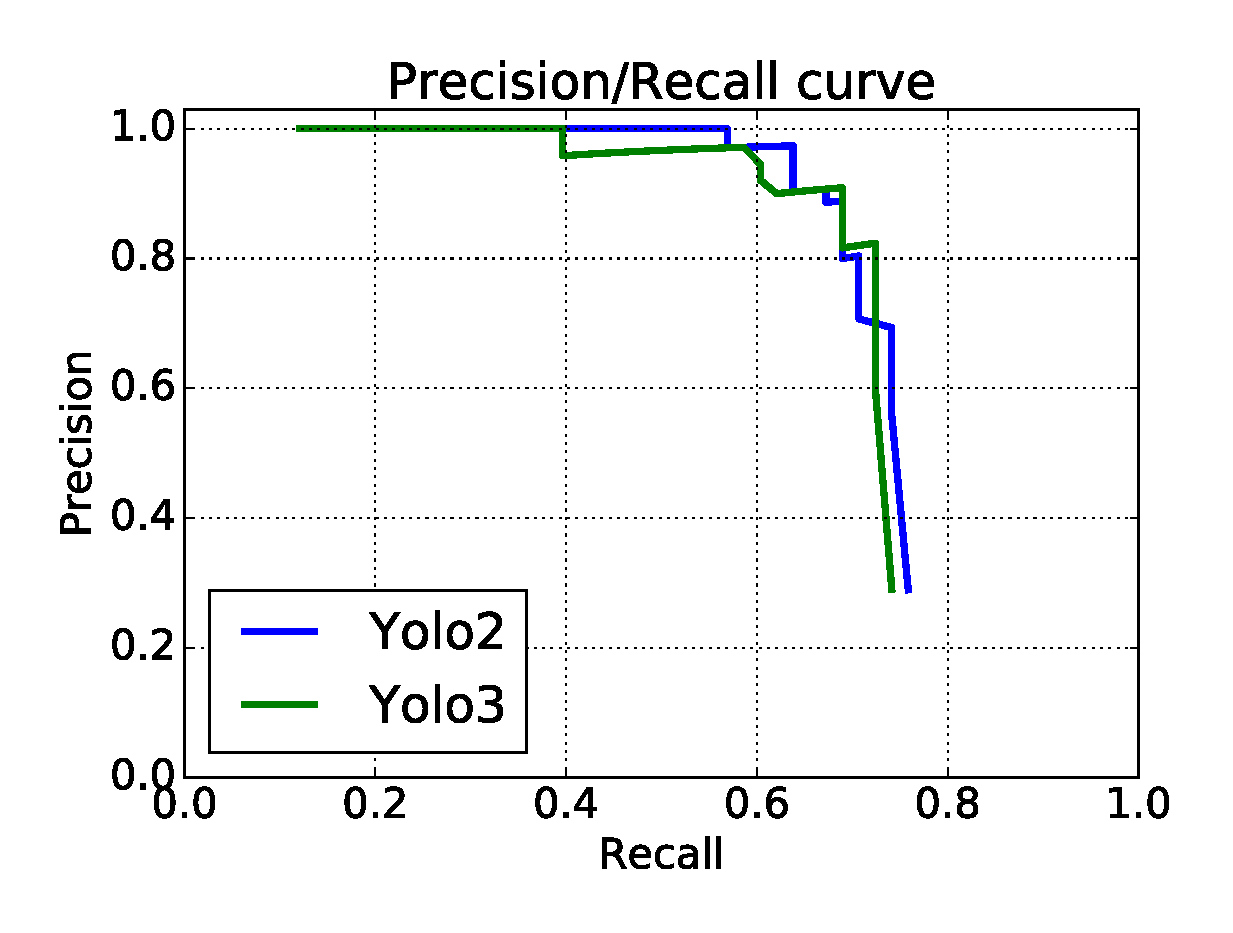
\includegraphics[width=0.8\linewidth]{results/case_buildings/prec_recall/yolo/bb.eps}
  \caption{Yolo tested on bbnb}
  \label{fig:sfig1}
\end{subfigure}%
\begin{subfigure}{.5\textwidth}
  \centering
  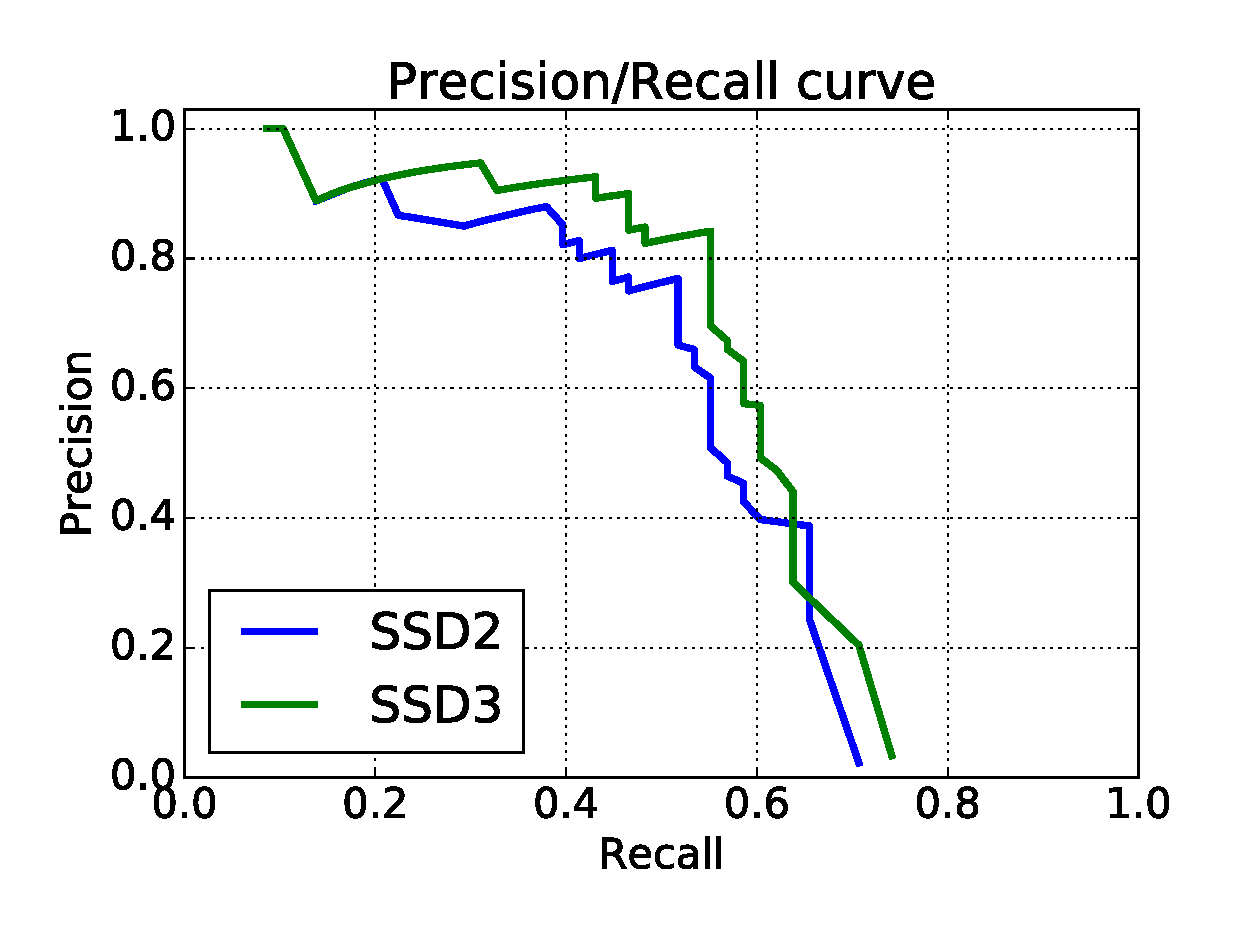
\includegraphics[width=.8\linewidth]{results/case_buildings/prec_recall/ssd/bb.eps}
  \caption{SSD tested on bbnb}
  \label{fig:sfig2}
\end{subfigure}

\begin{subfigure}{.5\textwidth}
  \centering
  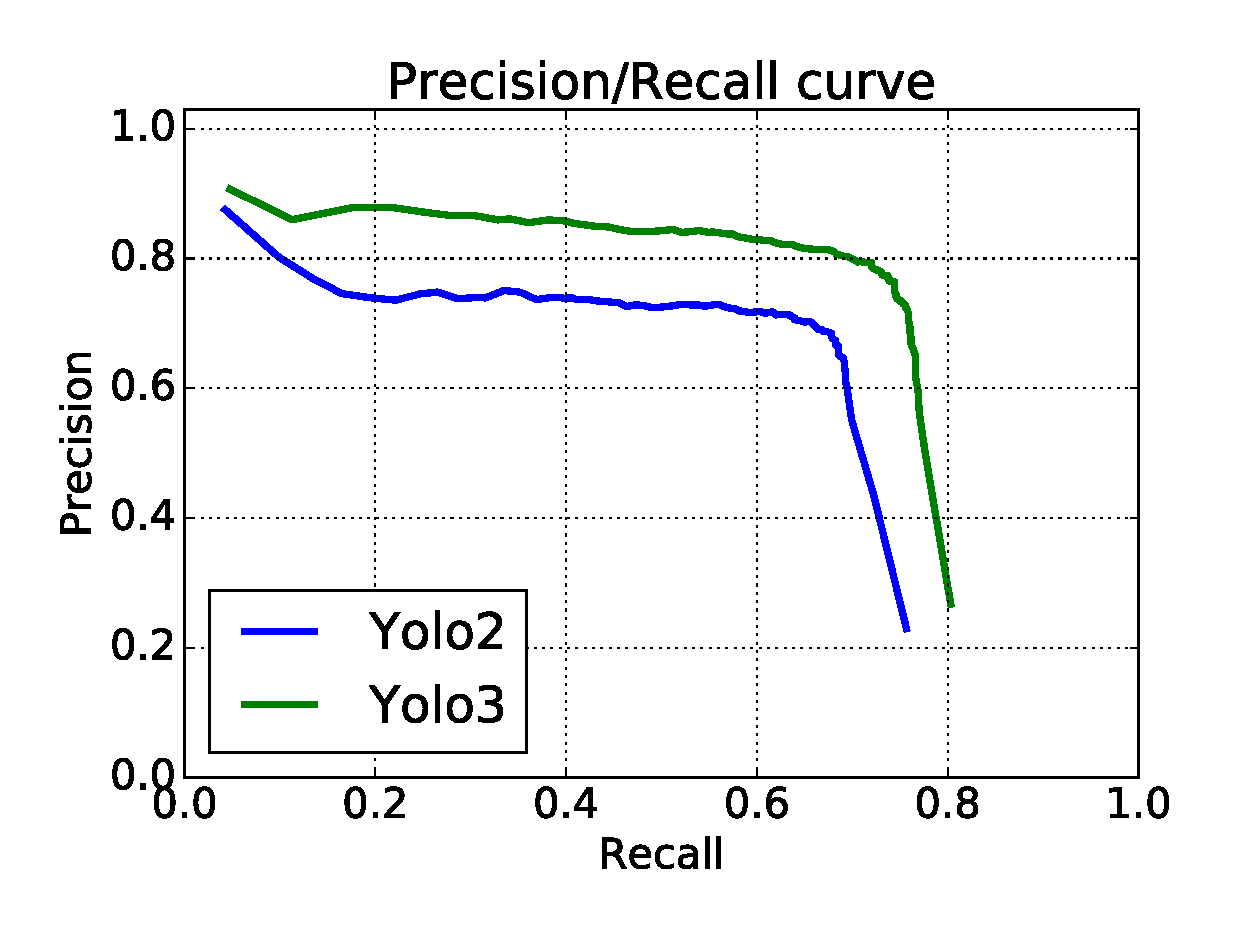
\includegraphics[width=0.8\linewidth]{results/case_buildings/prec_recall/yolo/bcbf.eps}
  \caption{Yolo tested on \textit{bc}, \textit{bf}}
  \label{fig:sfig1}
\end{subfigure}%
\begin{subfigure}{.5\textwidth}
  \centering
  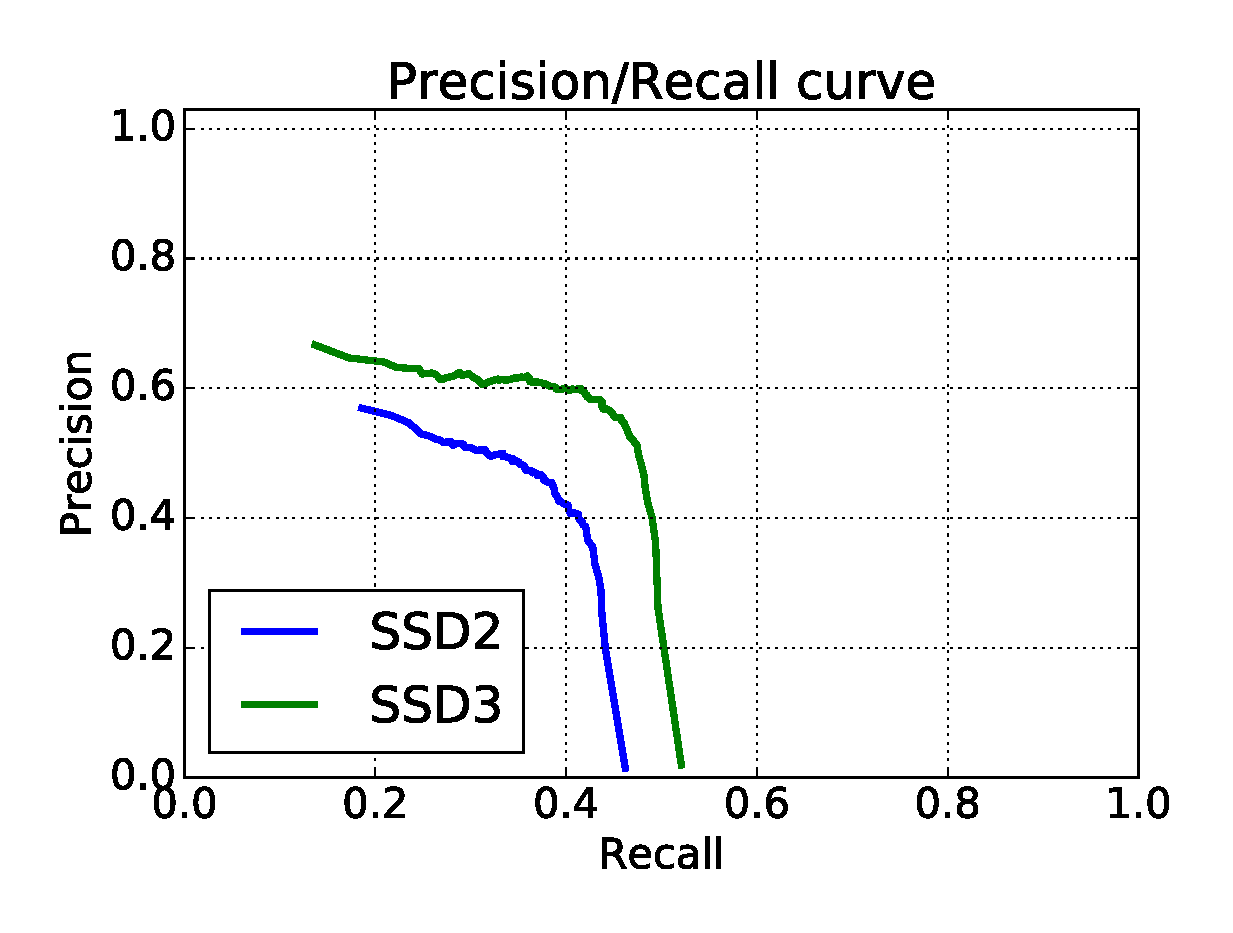
\includegraphics[width=.8\linewidth]{results/case_buildings/prec_recall/ssd/bcbf.eps}
  \caption{SSD tested on \textit{bc}, \textit{bf}}
  \label{fig:sfig2}
\end{subfigure}

\begin{subfigure}{.5\textwidth}
  \centering
  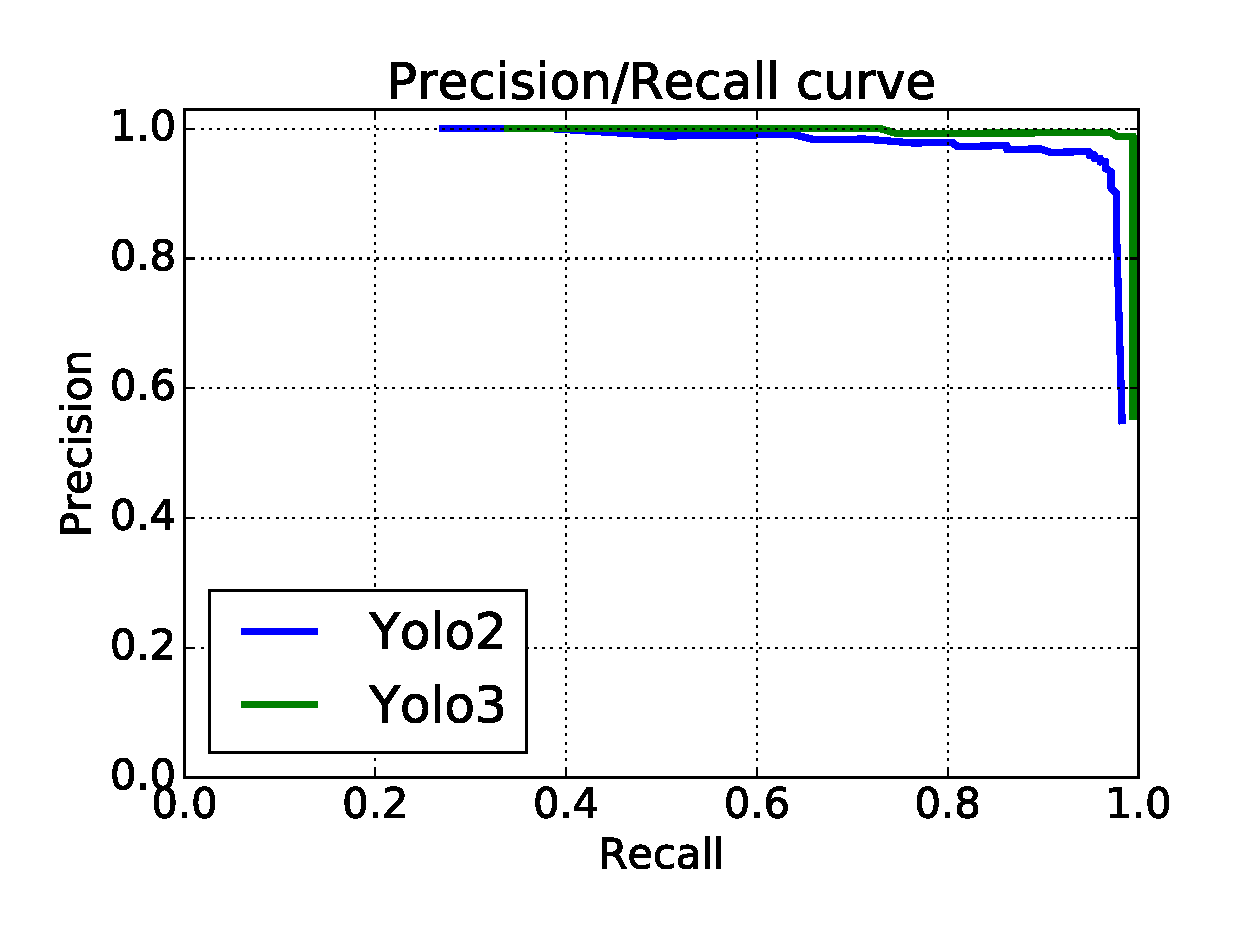
\includegraphics[width=0.8\linewidth]{results/case_buildings/prec_recall/yolo/trf.eps}
  \caption{Yolo tested on \textit{trf}}
  \label{fig:sfig1}
\end{subfigure}%
\begin{subfigure}{.5\textwidth}
  \centering
  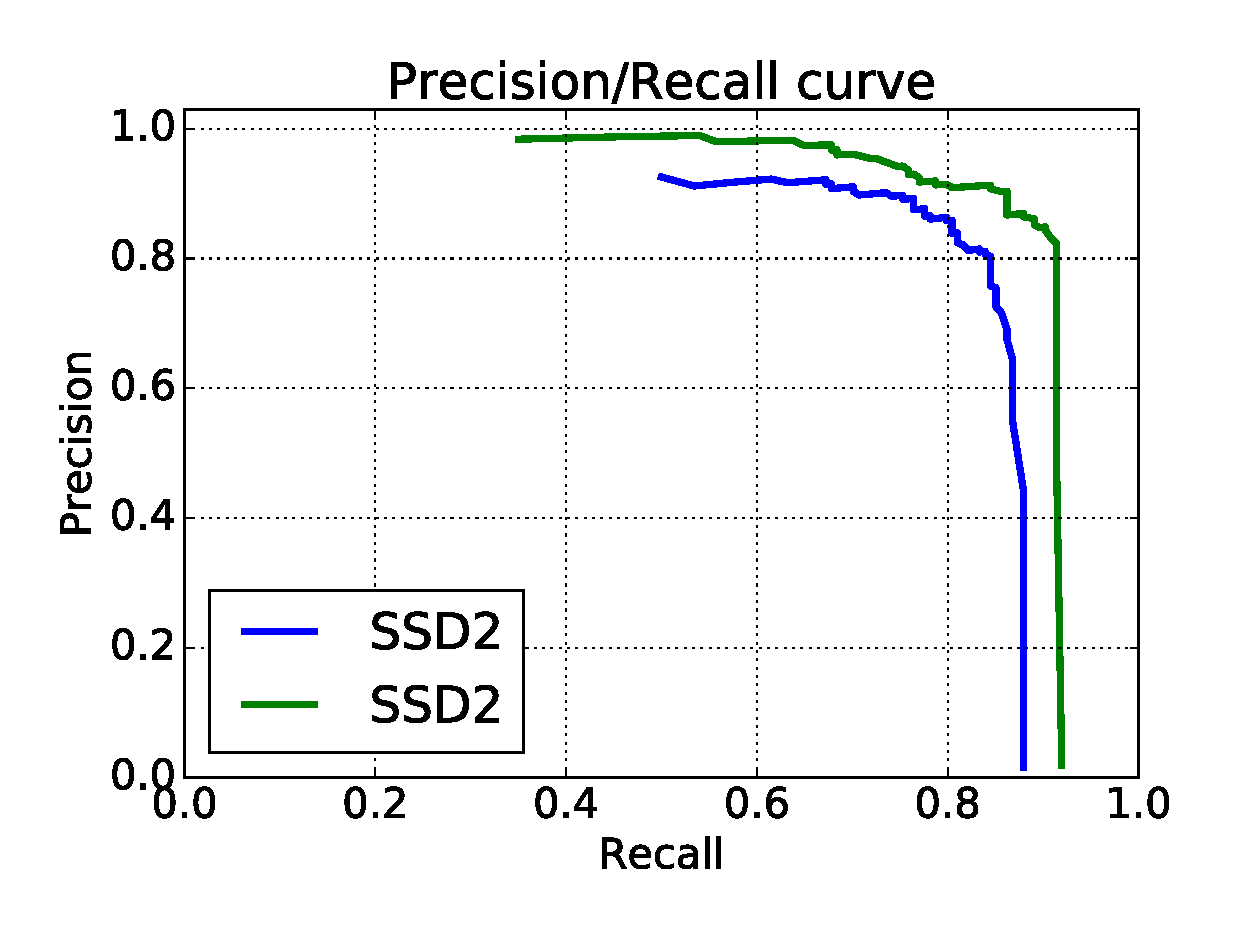
\includegraphics[width=.8\linewidth]{results/case_buildings/prec_recall/ssd/trf.eps}
  \caption{SSD tested on \textit{trf}}
  \label{fig:sfig2}
\end{subfigure}

\begin{subfigure}{.5\textwidth}
  \centering
  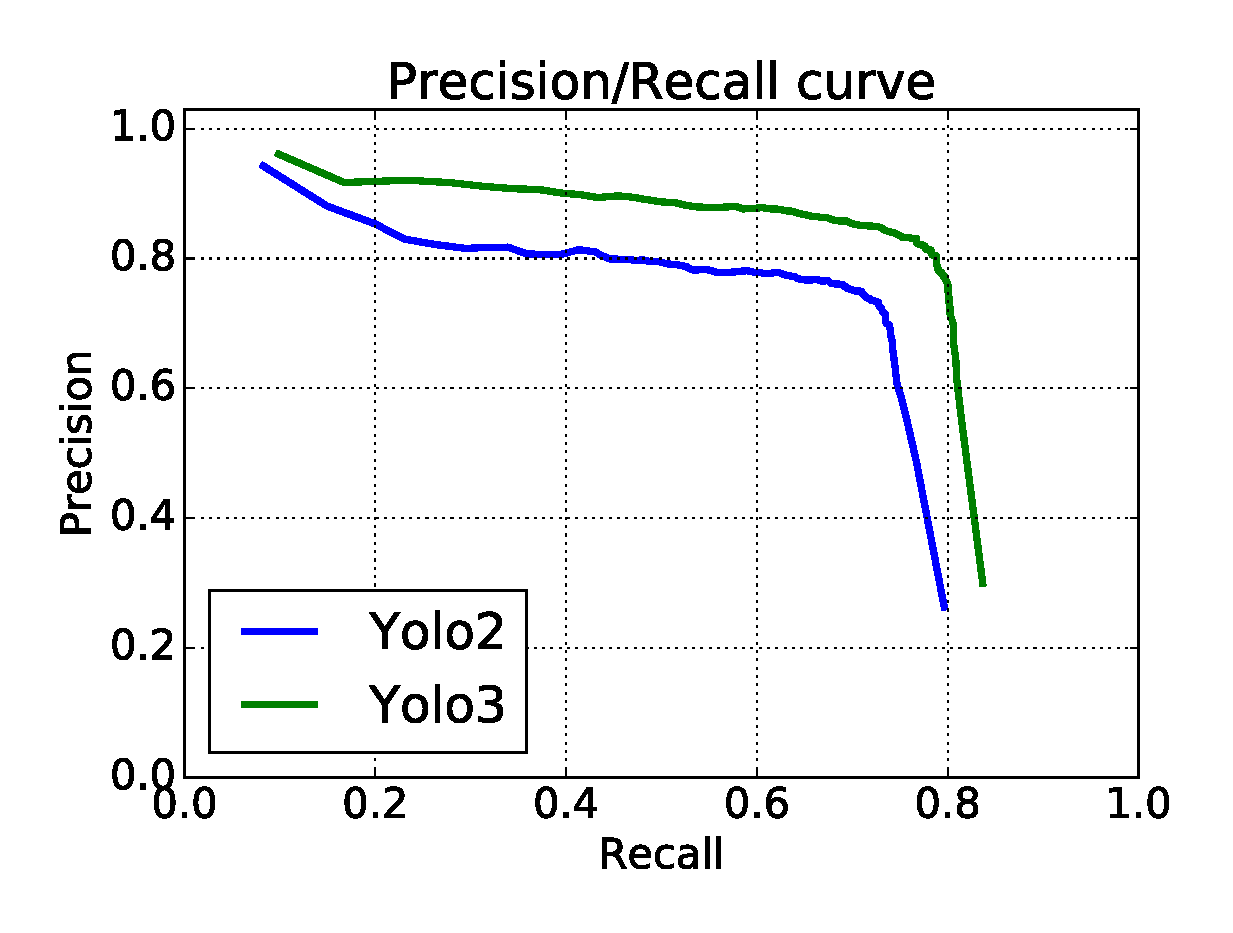
\includegraphics[width=0.8\linewidth]{results/case_buildings/prec_recall/yolo/bcbftrf.eps}
  \caption{Yolo tested on \textit{bc}, \textit{bf}, \textit{trf}}
  \label{fig:sfig1}
\end{subfigure}%
\begin{subfigure}{.5\textwidth}
  \centering
  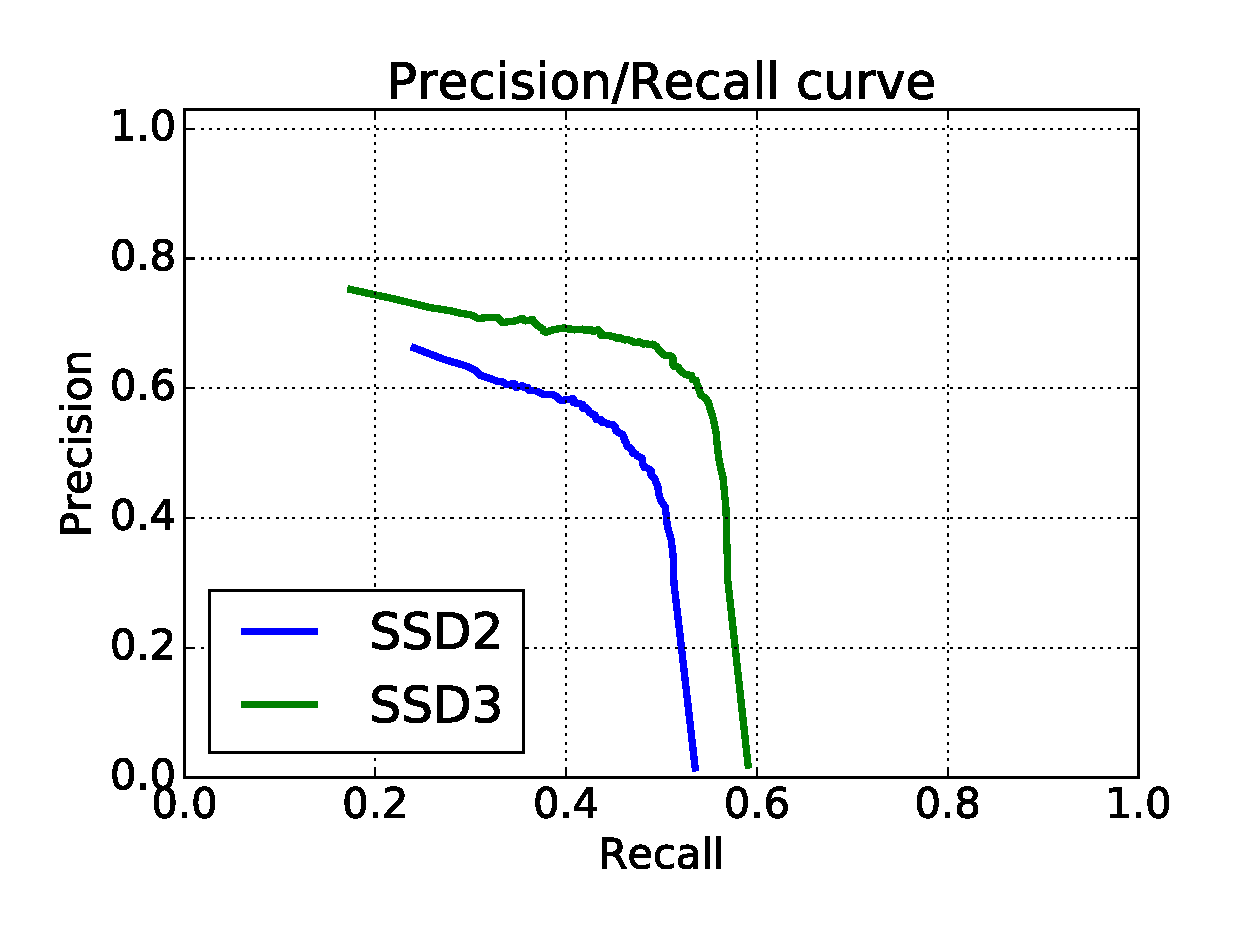
\includegraphics[width=.8\linewidth]{results/case_buildings/prec_recall/ssd/bcbftrf.eps}
  \caption{SSD tested on \textit{bc}, \textit{bf}, \textit{trf}}
  \label{fig:sfig2}
\end{subfigure}
\caption{Precision/recall curves of Yolo2, Yolo3, SSD2 and SSD3}
\label{fig:case_build}
\end{figure}

\newpage


\subsection{Tested on \textit{bbnb}}

The hypothesis before running the experiment was that the bbnb dataset would be the most positively affected by training on a building class. Since \textit{bbnb} consists of mostly moored boats, where there are images that contain buildings close to sea level one could suspect could be mistaken as boats, as shown in \ref{img:bbnb_ex}. The building in the bottom left corner is close to sea level, while also being relatively close in size to the boats compared to the other buildings in the image, which makes it a good candidate for a misclassification. However, neither Yolo2 nor SSD2 classifies this building as a boat. All the detectors, Yolo2, Yolo3, SSD2 and SSD3 detects all the boats in the image. Both SSD2 and SSD3 detects the rightmost boat two times, and the bounding box differences between Yolo2 and Yolo3 and between SSD2 and SSD3 are so insignificant that training on the building class does not seem to help improve performance on this particular image. Both Yolo3 and ssd3 detects the buildings in the image well, as can be seen in figure \ref{fig:ex_bbnb_yolo3} and \ref{fig:ex_bbnb_ssd3}.


\begin{figure}[h!]
\begin{subfigure}{.5\textwidth}
  \centering
  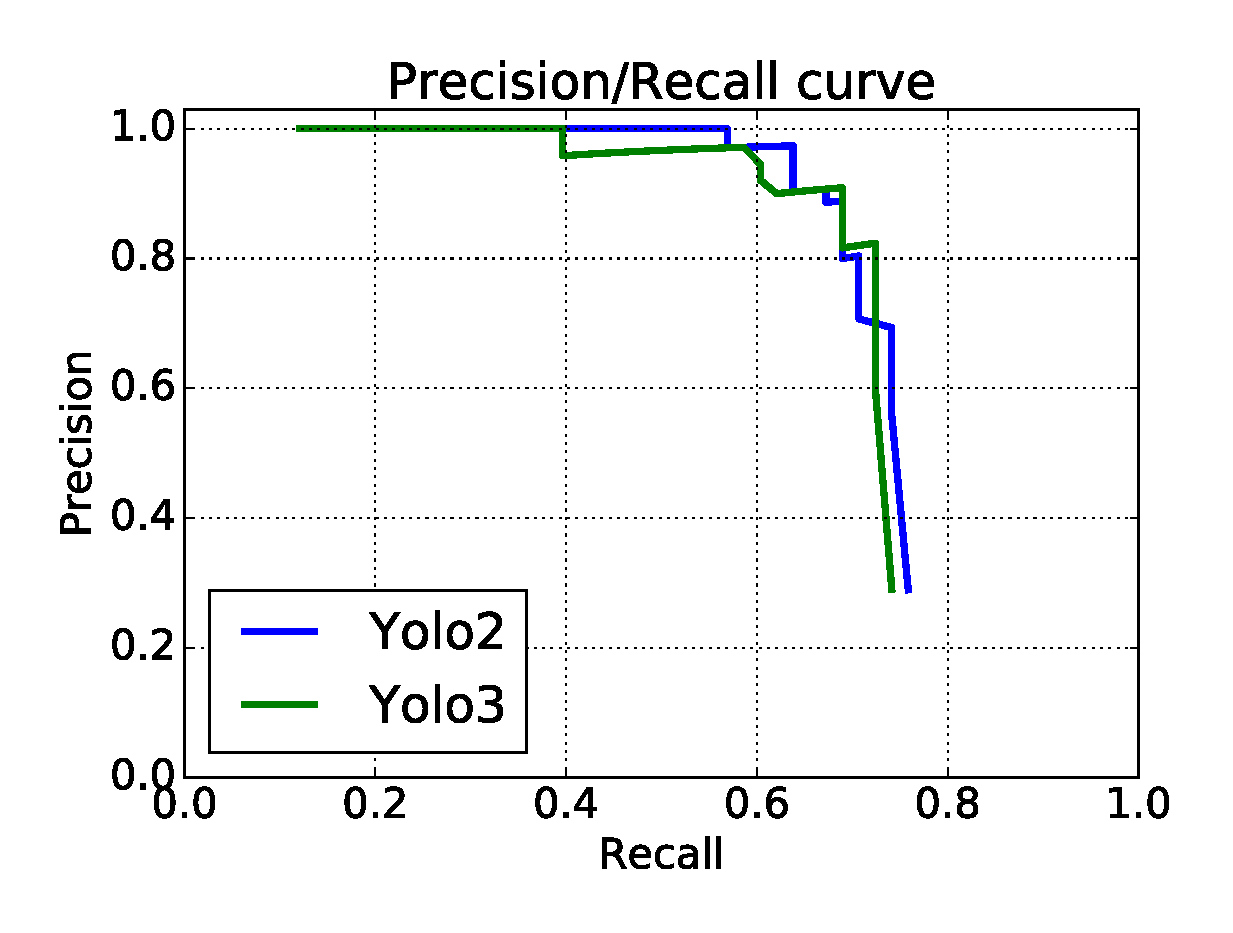
\includegraphics[width=0.8\linewidth]{results/case_buildings/prec_recall/yolo/bb.eps}
  \caption{Yolo tested on bbnb}
  \label{fig:ex_bnbb_prec_rec_yolo}
\end{subfigure}%
\begin{subfigure}{.5\textwidth}
  \centering
  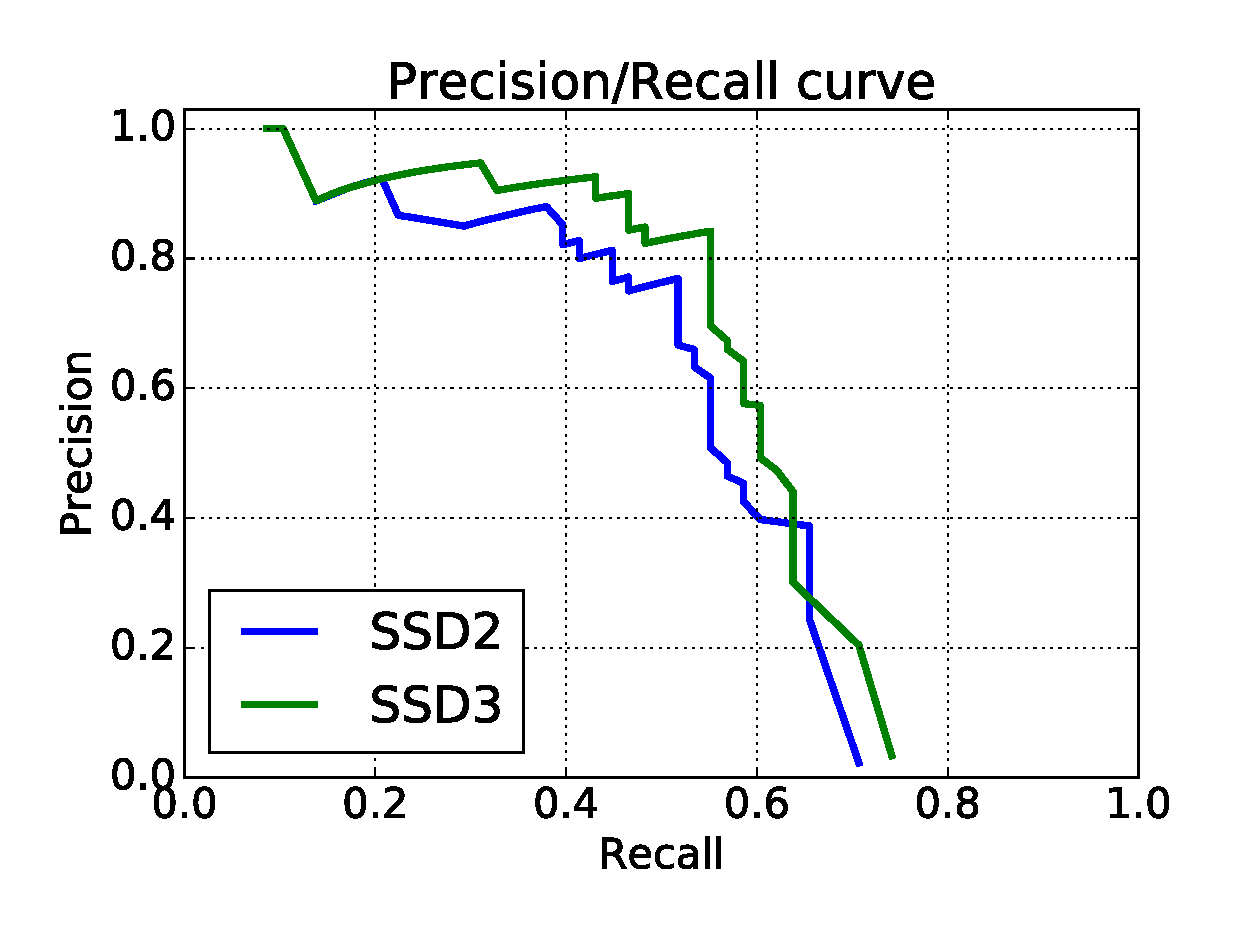
\includegraphics[width=.8\linewidth]{results/case_buildings/prec_recall/ssd/bb.eps}
  \caption{SSD tested on bbnb}
  \label{fig:ex_bnbb_prec_rec_ssd}
\end{subfigure}
\begin{subfigure}{.5\textwidth}
  \centering
  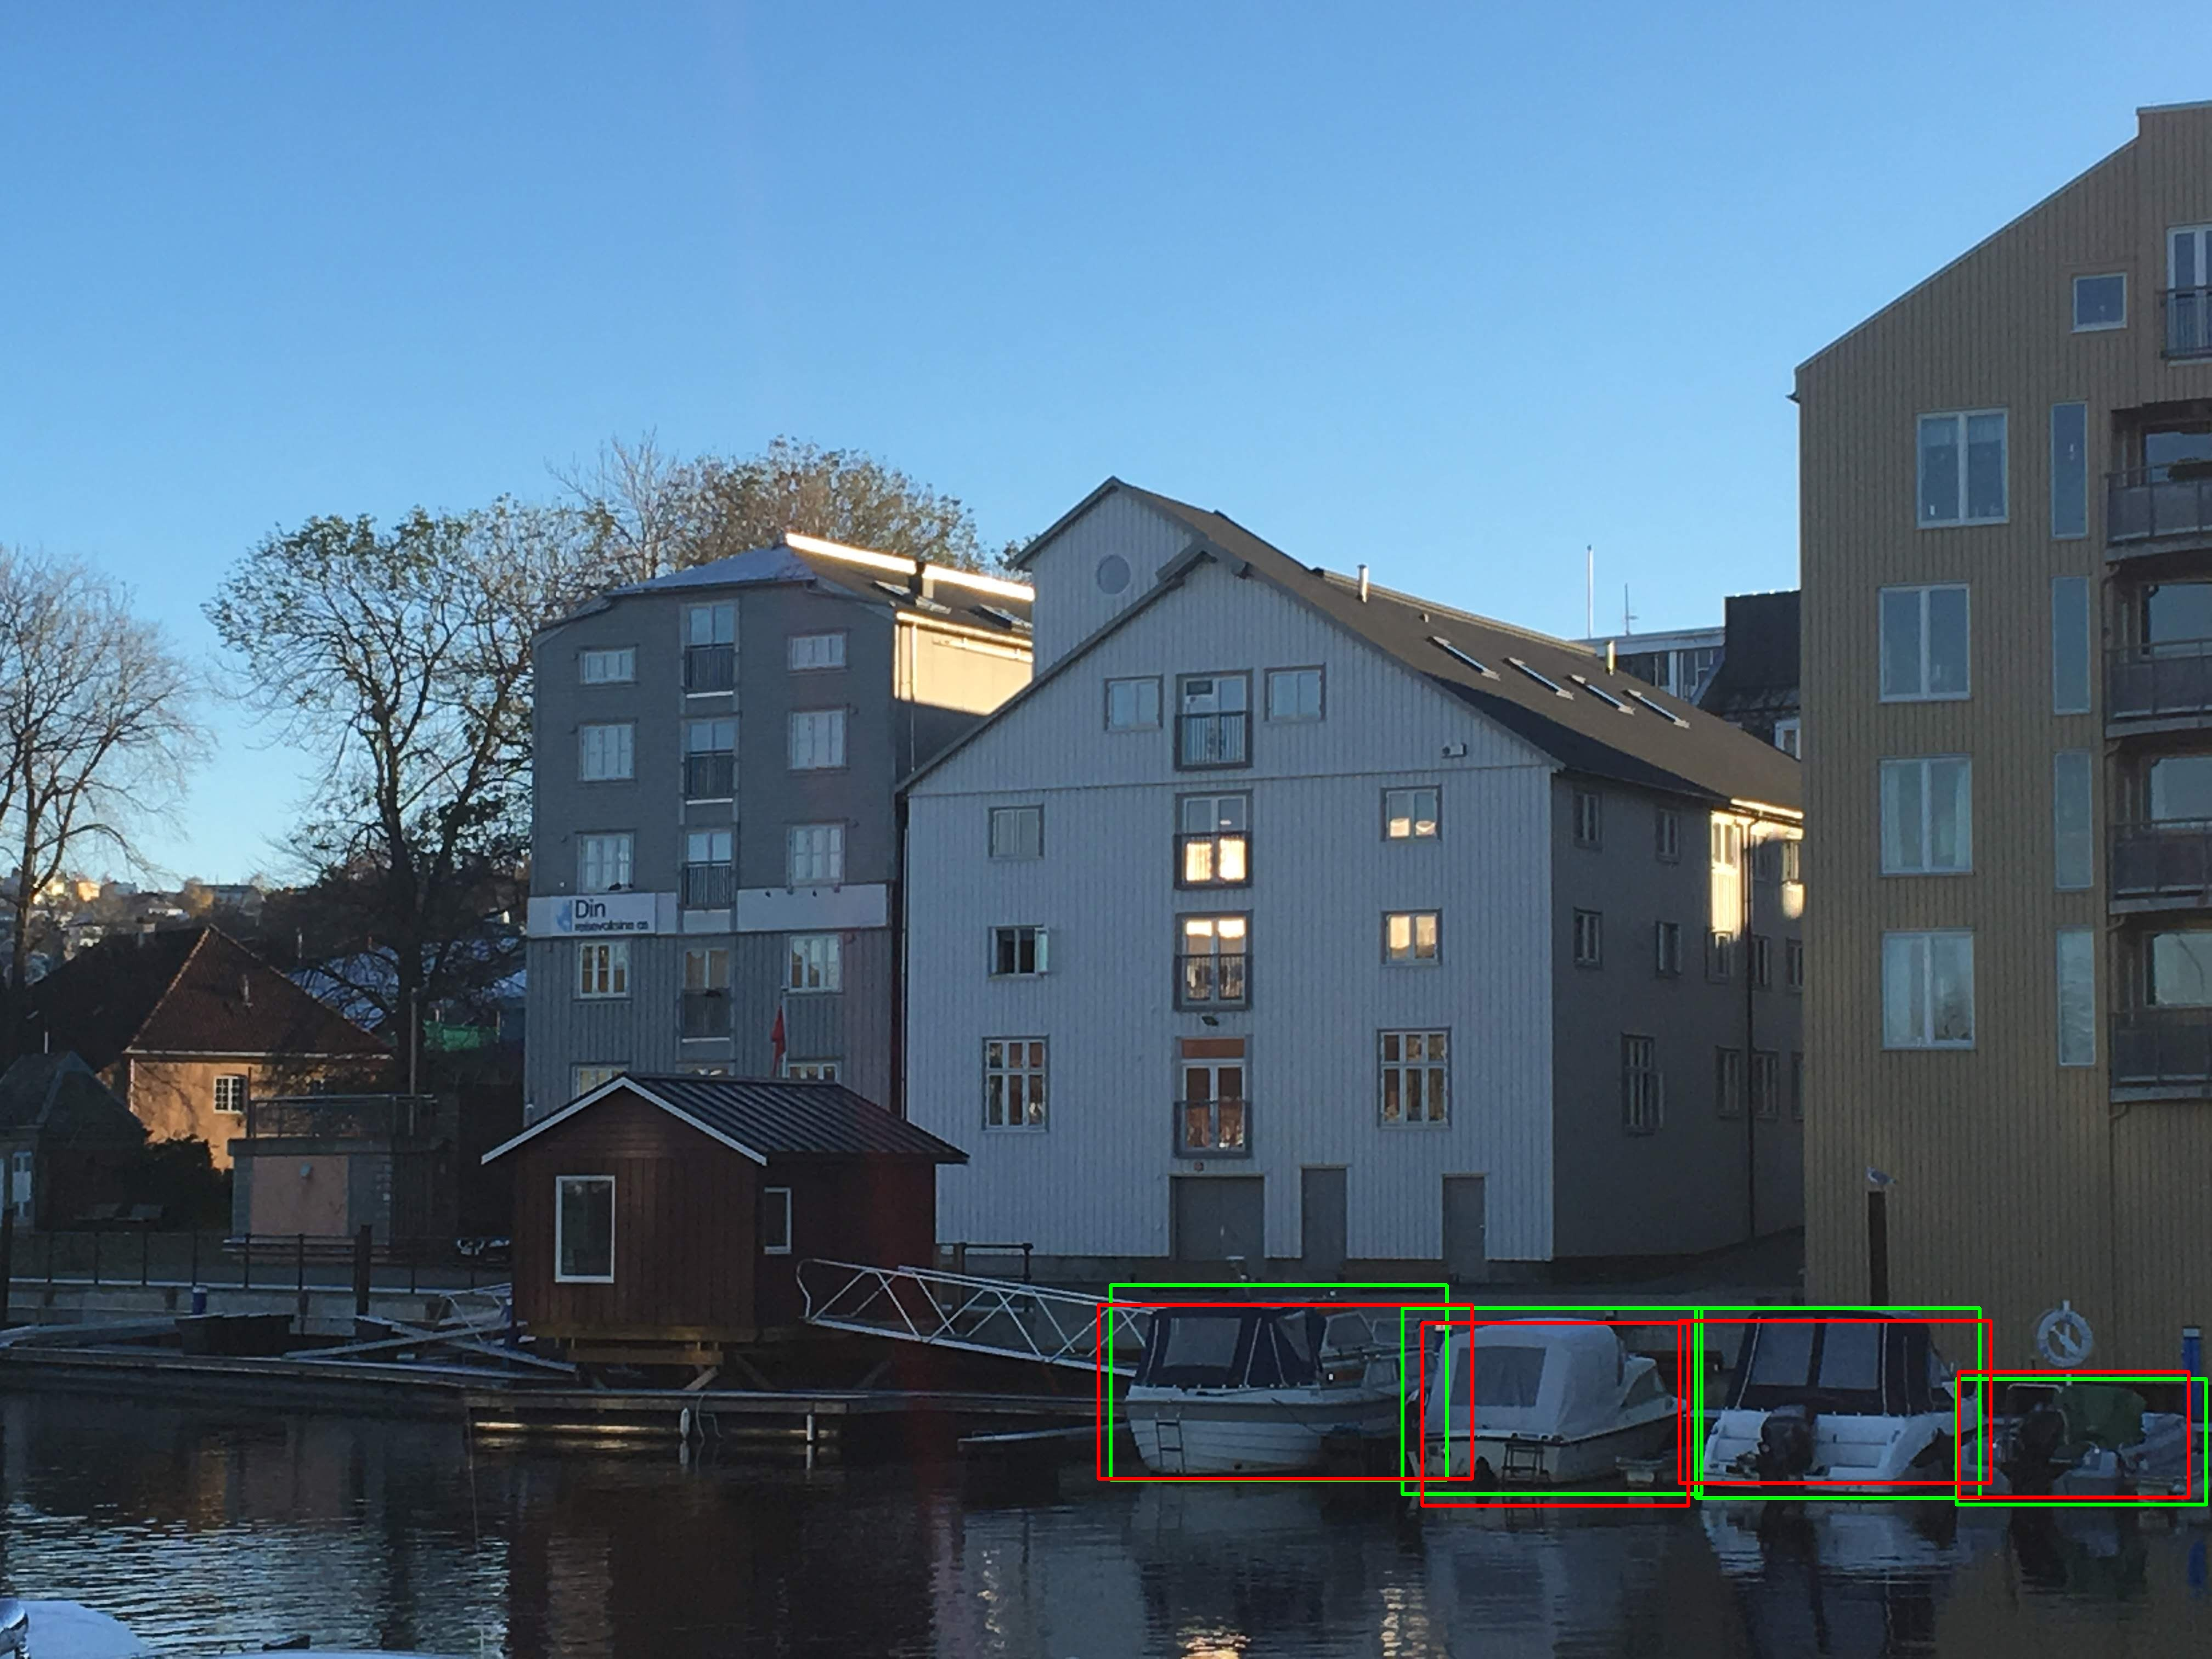
\includegraphics[width=0.8\linewidth]{results/case_buildings/prec_recall/yolo/IMG_2077_bbnb.jpg}
  \caption{Yolo2}
  \label{fig:ex_bbnb_yolo2}
\end{subfigure}%
\begin{subfigure}{.5\textwidth}
  \centering
  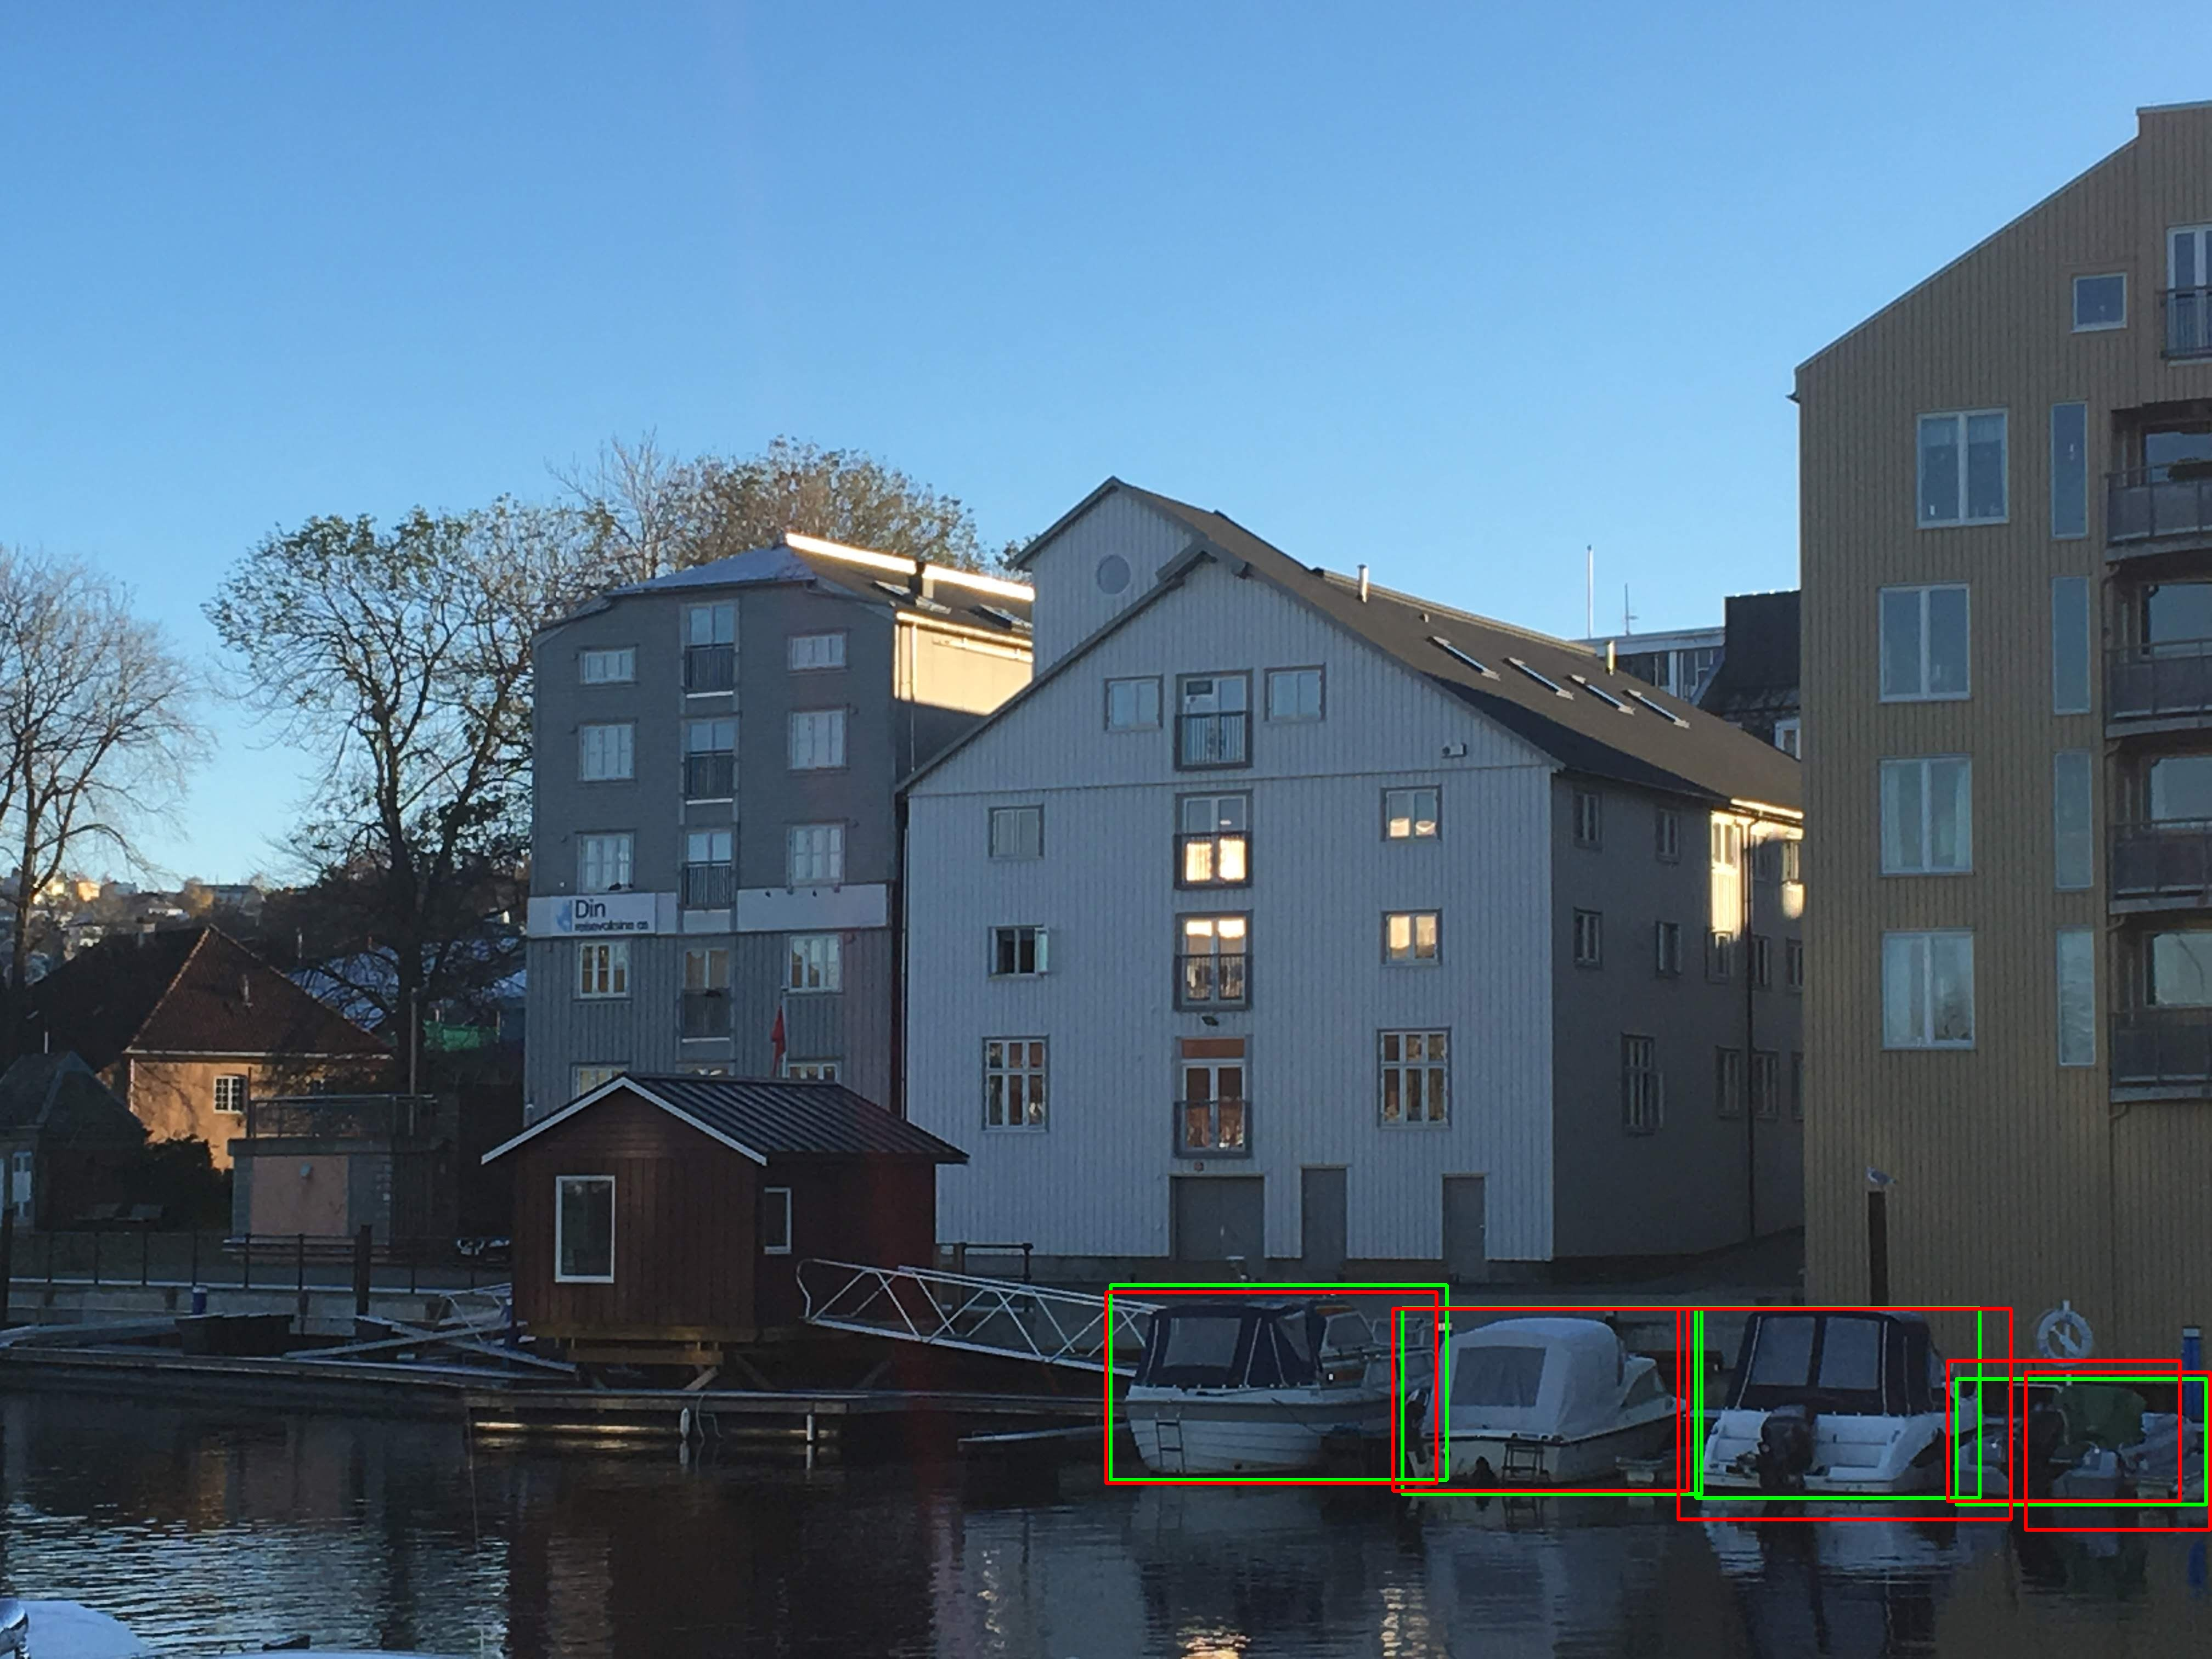
\includegraphics[width=.8\linewidth]{results/case_buildings/prec_recall/ssd/IMG_2077_bbnb.jpg}
  \caption{SSD2}
  \label{fig:ex_bbnb_ssd2}
\end{subfigure}

\begin{subfigure}{.5\textwidth}
  \centering
  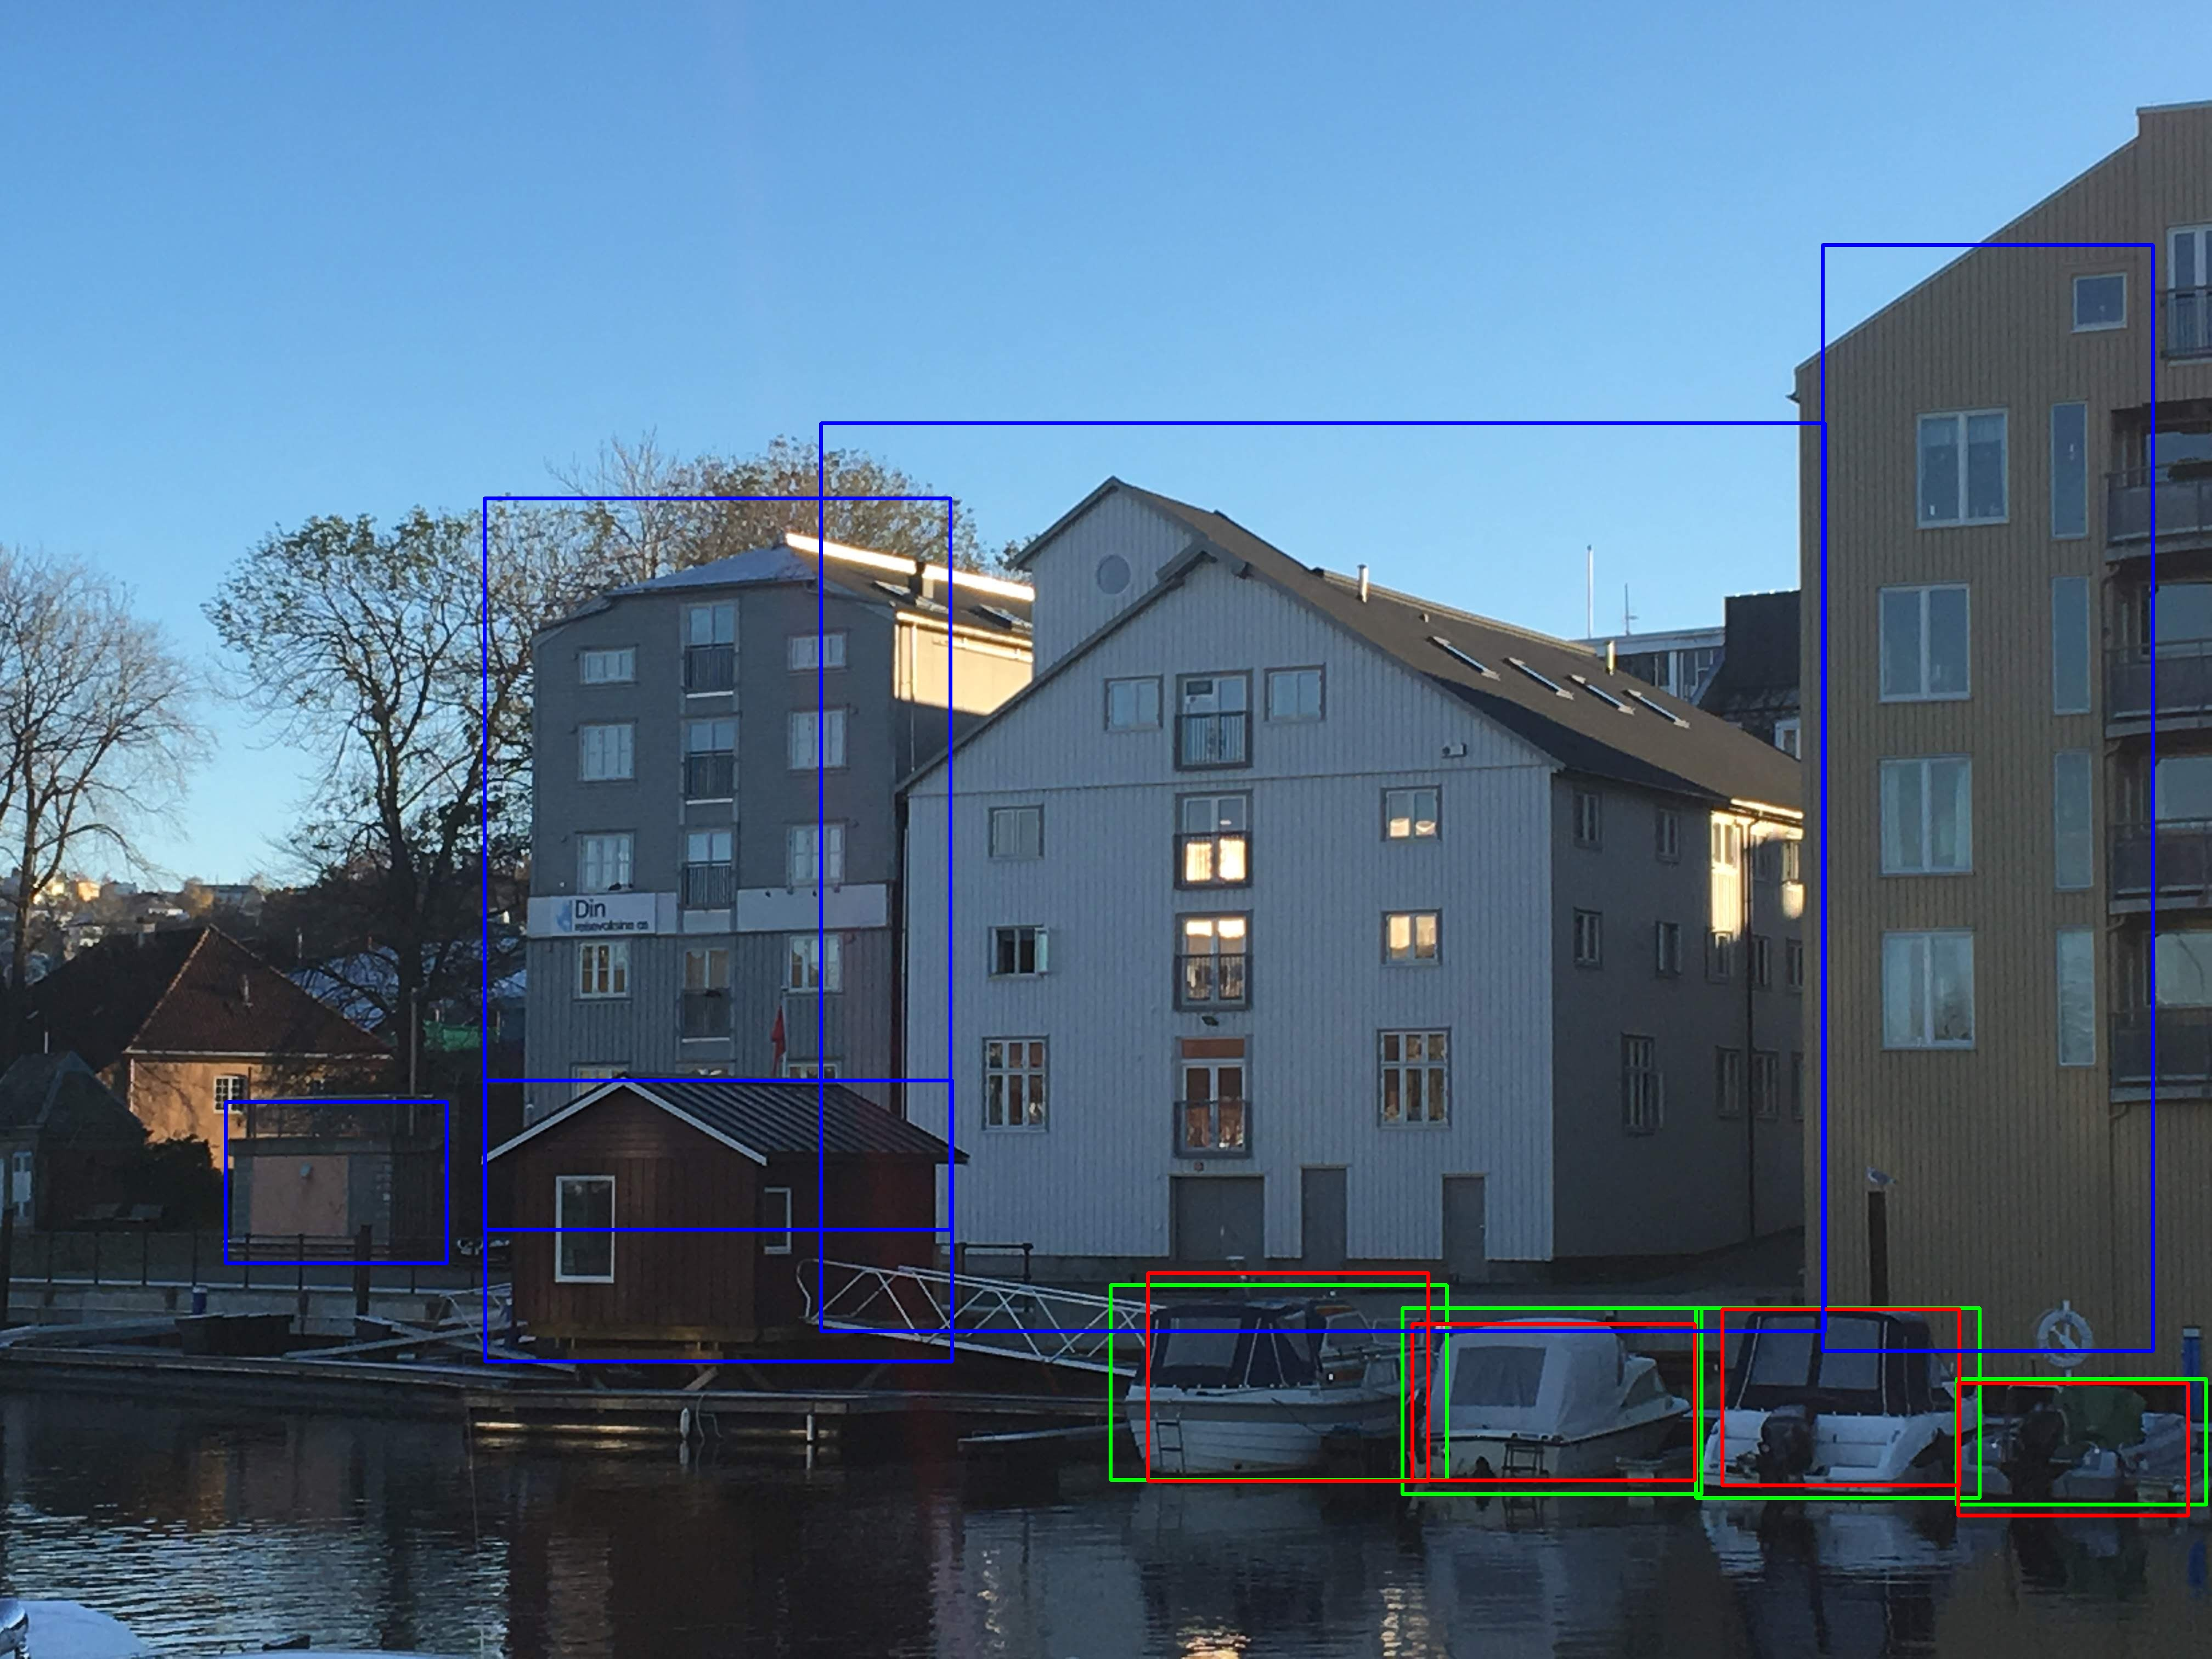
\includegraphics[width=0.8\linewidth]{results/case_buildings/prec_recall/yolo/IMG_2077_build.jpg}
  \caption{Yolo3}
  \label{fig:ex_bbnb_yolo3}
\end{subfigure}%
\begin{subfigure}{.5\textwidth}
  \centering
  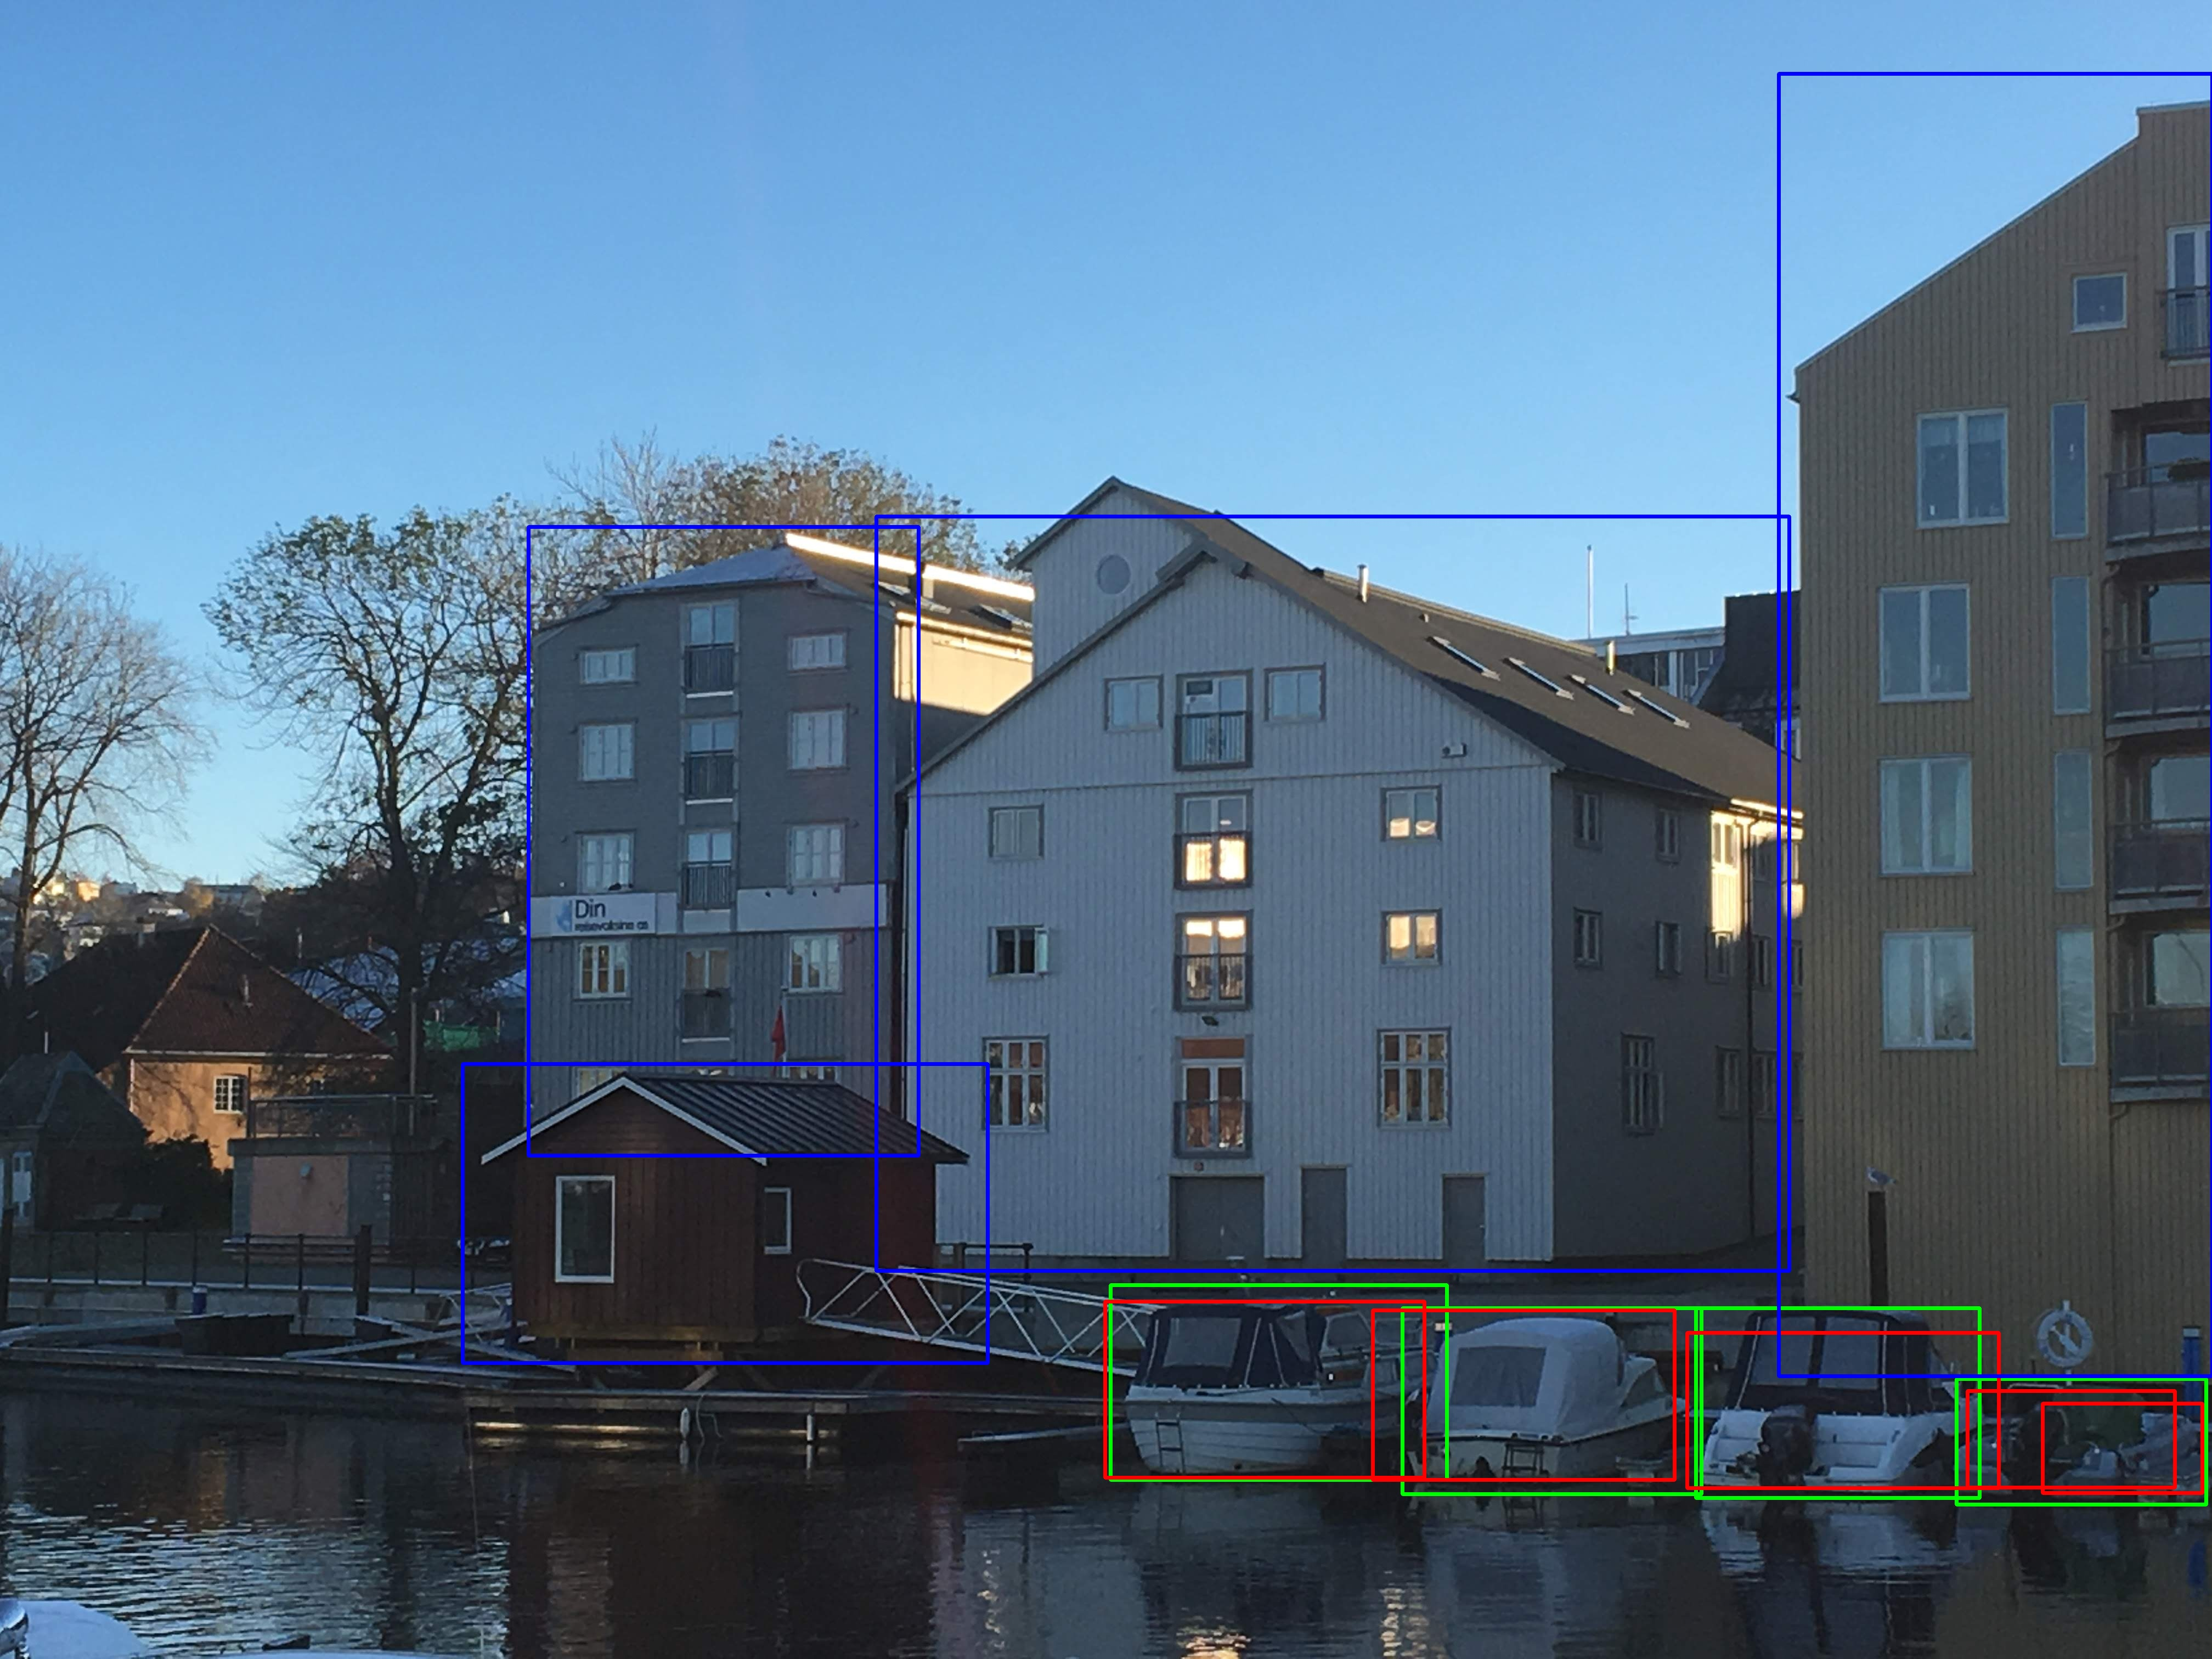
\includegraphics[width=.8\linewidth]{results/case_buildings/prec_recall/ssd/IMG_2077_build.jpg}
  \caption{SSD3}
  \label{fig:ex_bbnb_ssd3}
\end{subfigure}
\caption{Yolo2, Yolo3, SSD2, SSD3 example image from \textit{bbnb} test set. Green bounding boxes are ground truth, red bounding boxes are detected boats, blue bounding boxes are detected buildings}
\label{img:bbnb_ex}
\end{figure}

\newpage

\subsection{Tested on \textit{bc}, \textit{bf}}

The datasets \textit{bc} and \textit{bf} consists mostly of images taken towards open sea, of boats that are sailing, i.e., the boats are not moored. It is on this dataset the performance differences between Yolo2 and Yolo3 and between SSD2 and SSD3 differ the most, as can be seen in figure \ref{fig:bcbf_prec}.

\begin{figure}[h!]
\begin{subfigure}{.5\textwidth}
  \centering
  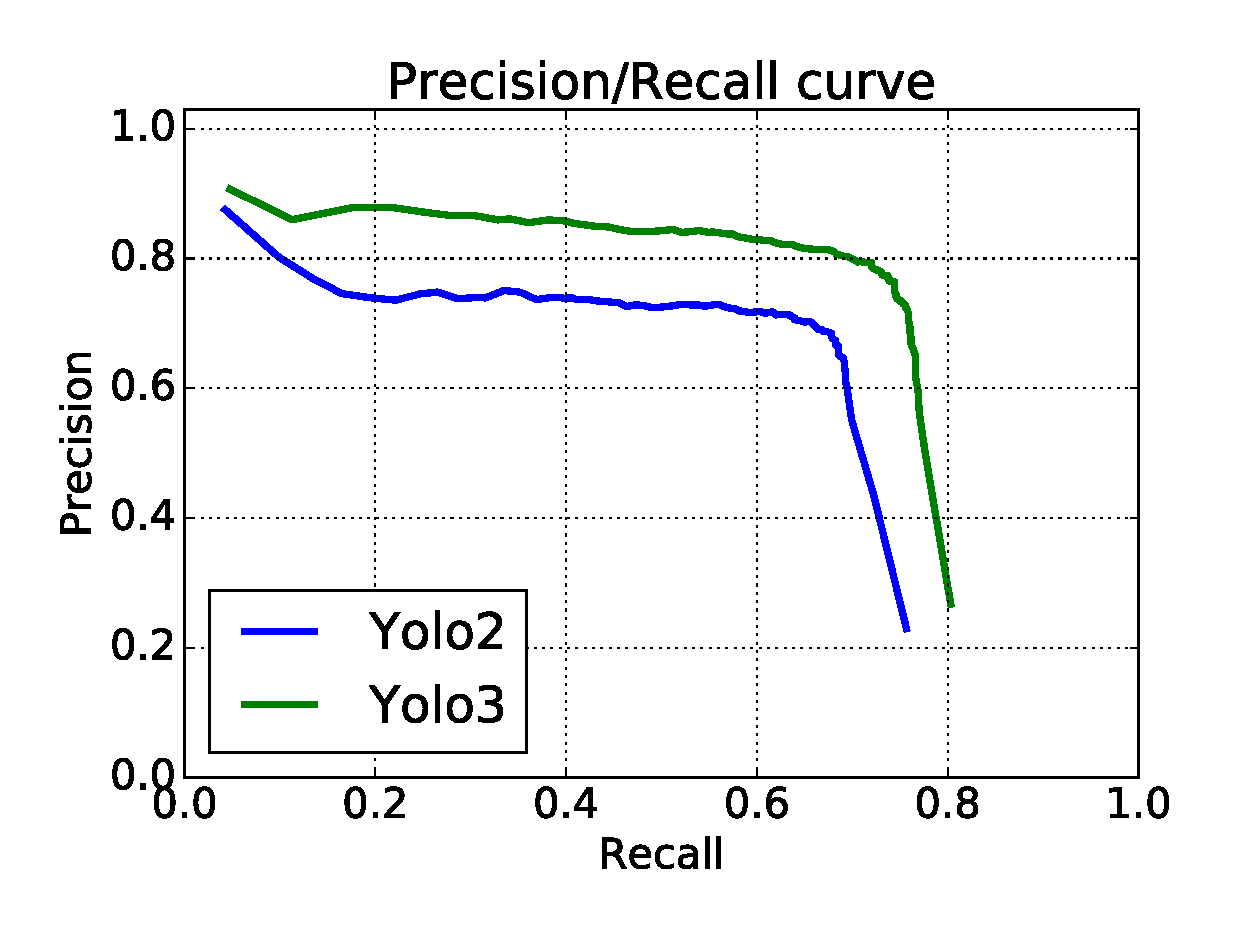
\includegraphics[width=0.8\linewidth]{results/case_buildings/prec_recall/yolo/bcbf.eps}
  \caption{Yolo tested on \textit{bc}, \textit{bf}}
  \label{fig:ex_bcbf_prec_rec_yolo}
\end{subfigure}%
\begin{subfigure}{.5\textwidth}
  \centering
  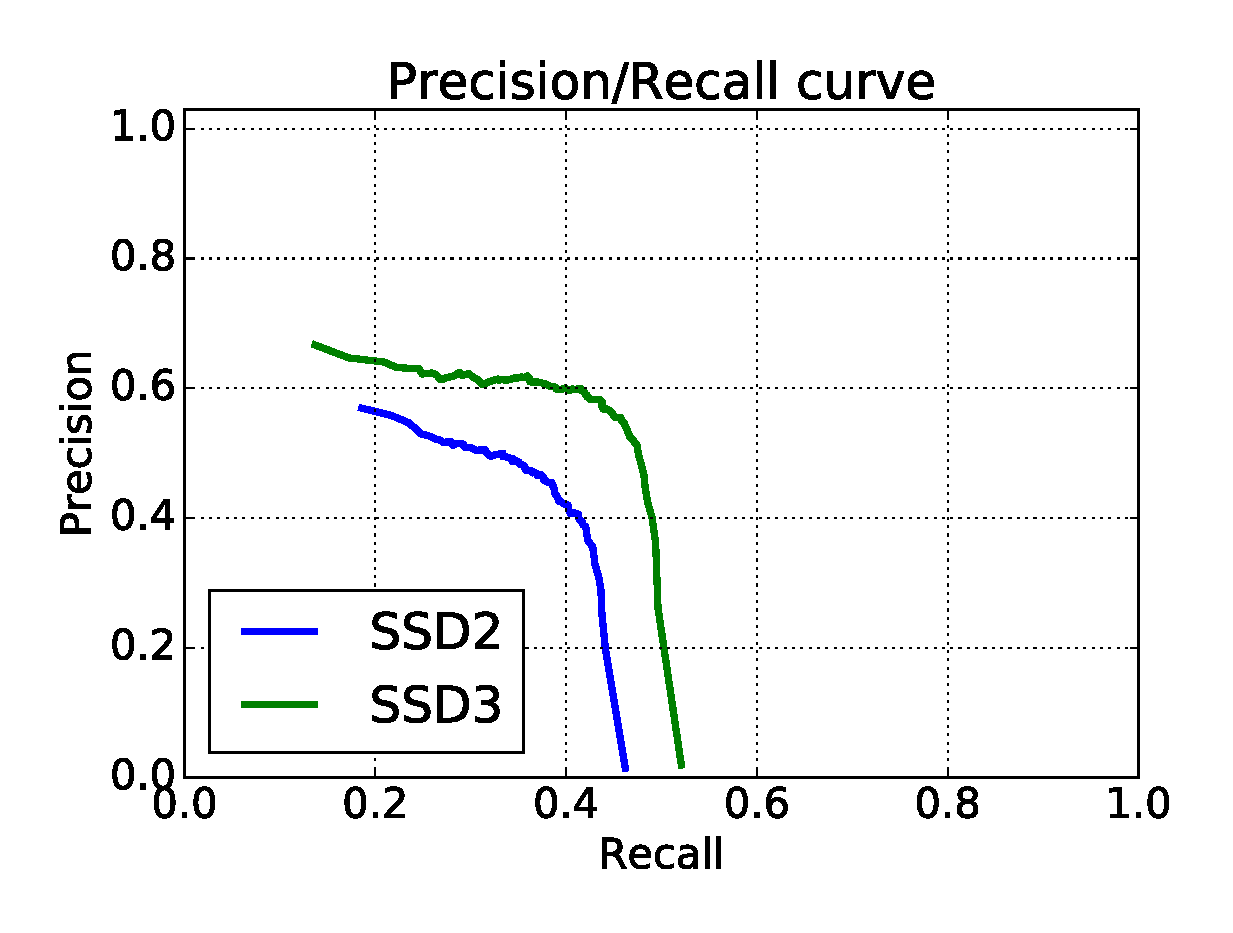
\includegraphics[width=.8\linewidth]{results/case_buildings/prec_recall/ssd/bcbf.eps}
  \caption{SSD tested on \textit{bc}, \textit{bf}}
  \label{fig:ex_bcbf_prec_rec_ssd}
\end{subfigure}
\caption{Yolo2, Yolo3, SSD2, SSD3 example image from \textit{bbnb} test set. Green bounding boxes are ground truth, red bounding boxes are detected boats, blue bounding boxes are detected buildings}
\label{fig:bcbf_prec}
\end{figure}

\vspace{3mm}

By going through the approximately 300 test images, some differences between the models become apparent. While the differences between SSD2 and SSD3 are somewhat obvious, the difference between Yolo2 and Yolo3 are more nuanced. 

\subsubsection{SSD2 and SSD3 on \textit{bc}, \textit{bf}}
In around 10 percent of the test images, SSD2 detects land as a boat, in none of these images does SSD3 perform the same way. An example of this is shown in figure \ref{img:bixbox_ssd}. More examples of this behavior can be found in Appendix C in chapter \ref{sec:bigbox}

\begin{figure}[h!]
\begin{subfigure}{.5\textwidth}
  \centering
  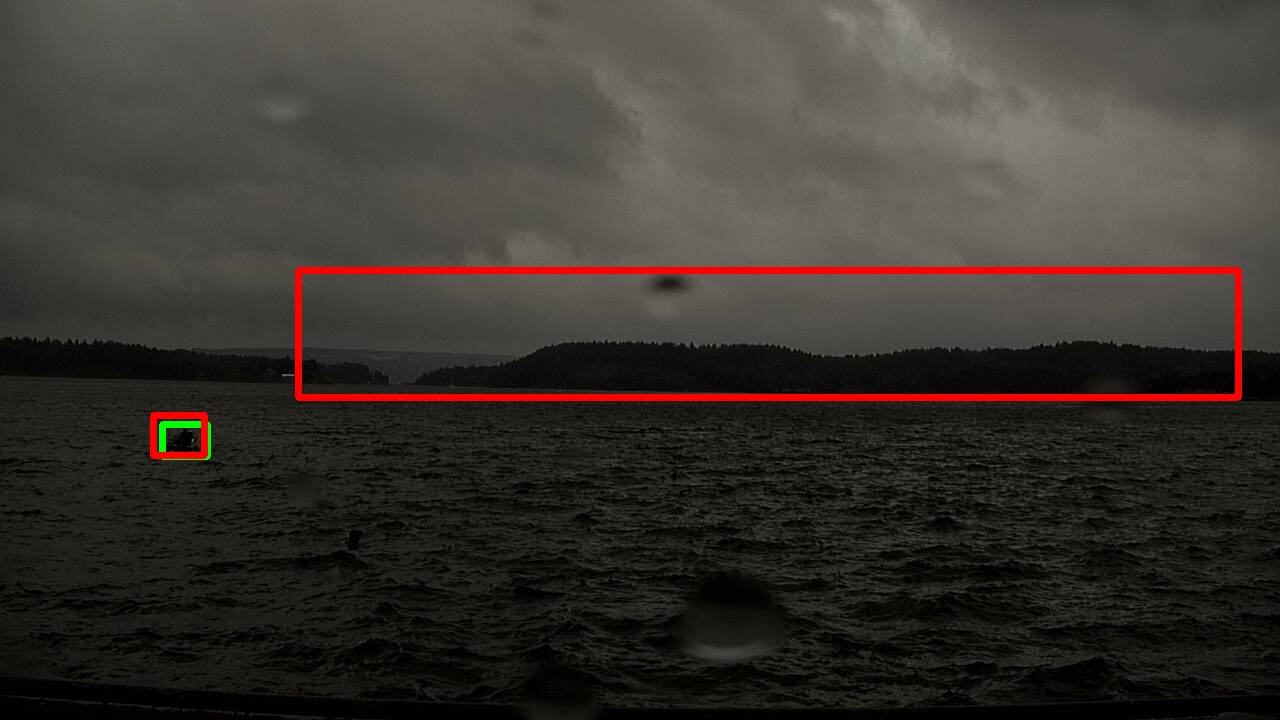
\includegraphics[width=0.9\linewidth]{results/case_buildings/bigbox_bcbf/SSD2/selected_06_14_axis0049.jpg}
  \caption{SSD2}
  \label{fig:big_box_ssd2}
\end{subfigure}%
\begin{subfigure}{.5\textwidth}
  \centering
  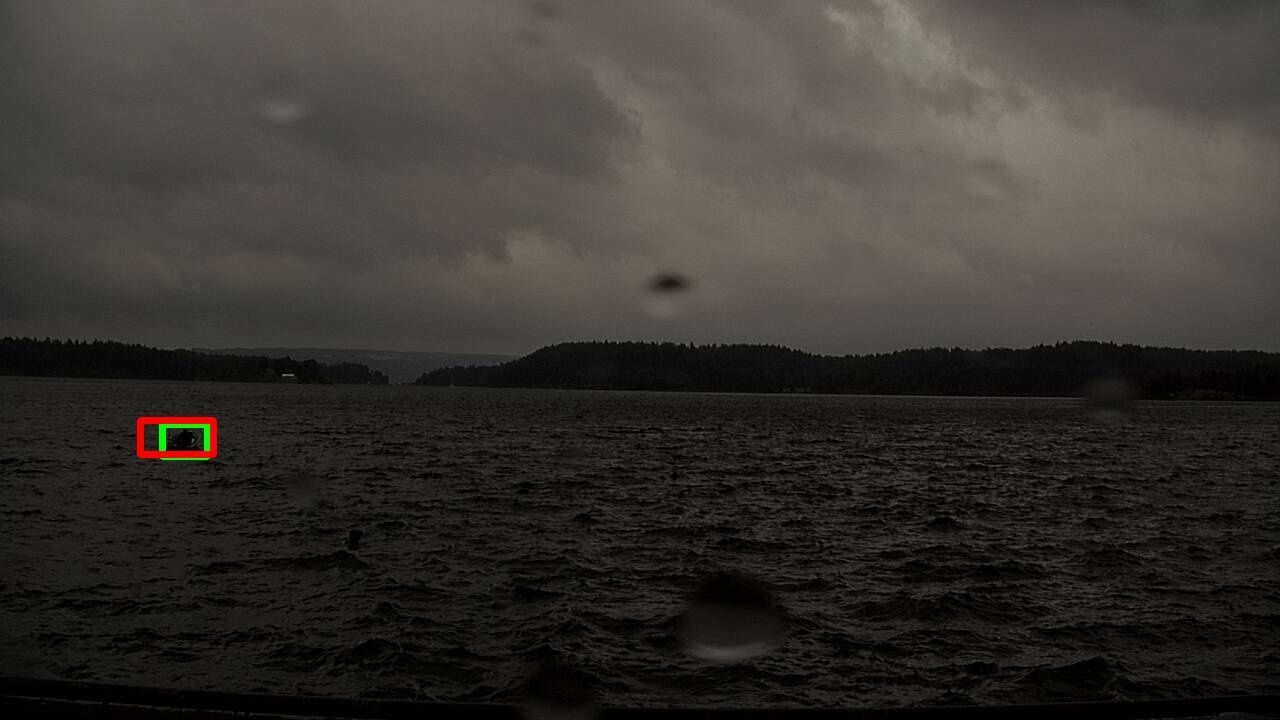
\includegraphics[width=.9\linewidth]{results/case_buildings/bigbox_bcbf/SSD3/selected_06_14_axis0049.jpg}
  \caption{SSD3}
  \label{fig:big_box_ssd3}
\end{subfigure}
\caption{SSD2 detects land as boat. Red bounding boxes are boat detections, green bounding boxes are ground truth.}
\label{img:bixbox_ssd}
\end{figure}

There are also some examples where SSD2 misclassifies buildings as boats, while SSD3 does not. One example is shown in figure \ref{img:misclass_ssd}

\begin{figure}[h!]
\begin{subfigure}{.5\textwidth}
  \centering
  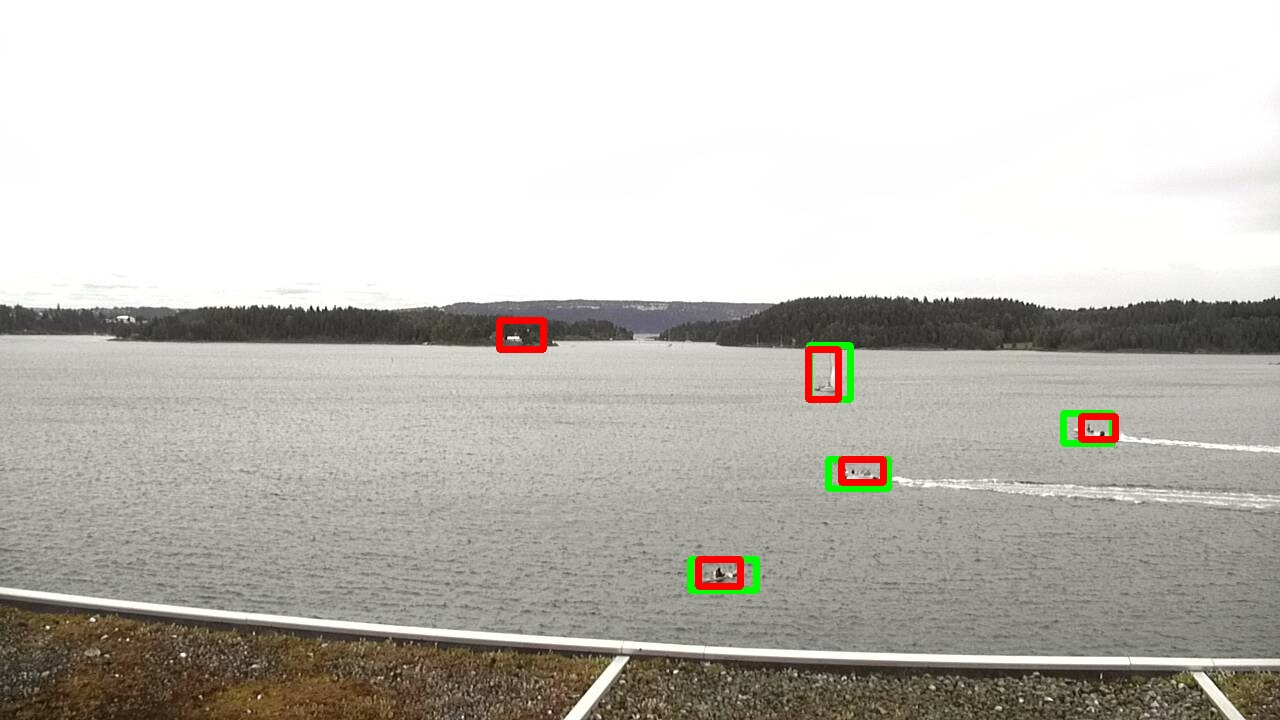
\includegraphics[width=0.9\linewidth]{results/case_buildings/misclass/selected_08_07_frame11982_bbnb.jpg}
  \caption{SSD2}
  \label{fig:misclass_ssd2}
\end{subfigure}%
\begin{subfigure}{.5\textwidth}
  \centering
  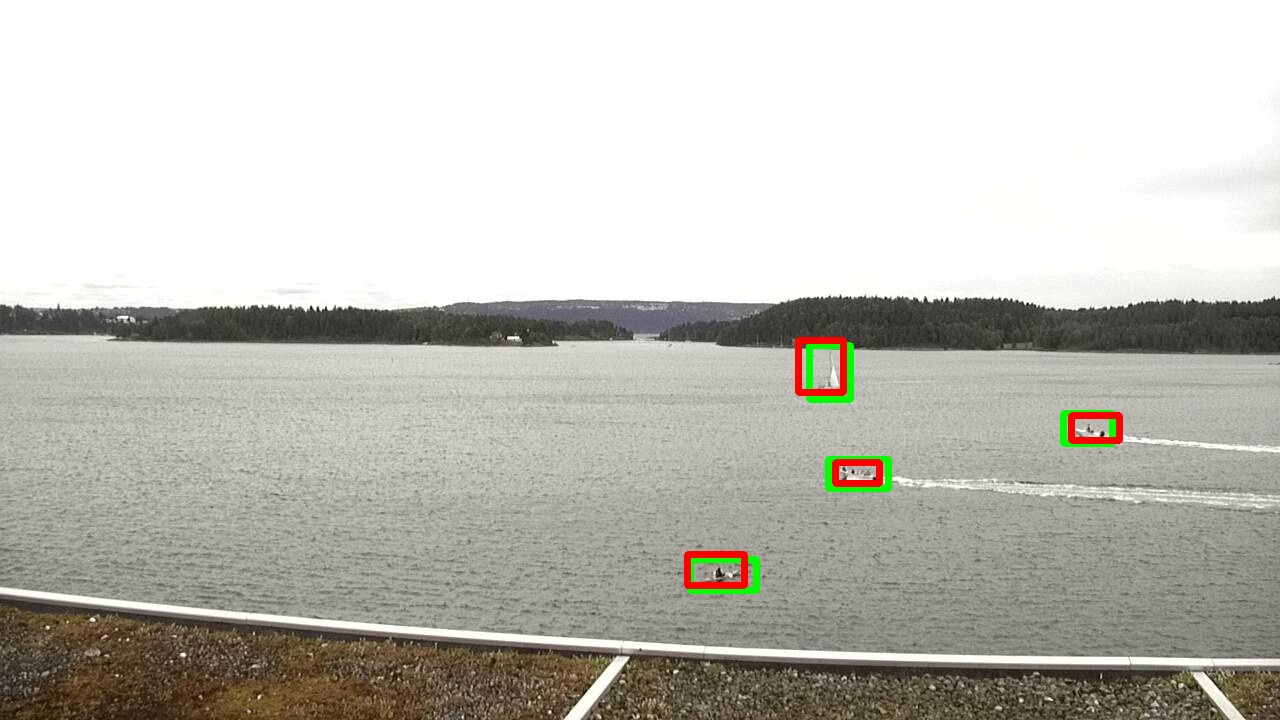
\includegraphics[width=.9\linewidth]{results/case_buildings/misclass/selected_08_07_frame11982_build.jpg}
  \caption{SSD3}
  \label{fig:misclass_ssd3}
\end{subfigure}
\caption{Leftmost red bounding box in SSD2 is a detection of a building as a boat, this is not detected as a boat in SSD3. Red bounding boxes are boat detections, green bounding boxes are ground truth.}
\label{img:misclass_ssd}
\end{figure}

\vspace{3mm}
\newpage

\subsubsection{Yolo2 and Yolo3 on \textit{bc}, \textit{bf}}

As mentioned Yolo2 and Yolo3 does not differ as clearly as SSD2 and SSD3. There are examples of Yolo2 performing better than Yolo3 and vice versa. In many of the misclassifications in the test data both Yolo2 and Yolo3 mistakes the same object as a boat. By analyzing the results from both Yolo2 and Yolo3, the following tendencies can be seen:

\begin{itemize}
    \item Yolo2 and Yolo3 have the disposition to wrongly classify the same objects as boats. See Appendix C chapter \ref{sec:same_mistake} for example images.
    \item Yolo2 performs better in some cases, while Yolo3 performs better in other. It is not clear what makes one better than the other in each specific case. See Appendix C chapter \ref{sec:3better} and \ref{sec:2better} for example images
    \item Yolo2 makes some misclassifications that could imply that training on a building class makes Yolo3 more robust to the more incomprehensible misclassifications. See appendix C chapter \ref{sec:yolo2_spec_misc} for example images.
\end{itemize}

As opposed to the differences between SSD2 and SSD3 the differences in the results between Yolo2 and Yolo3 are hard to pinpoint. Both Yolo2 and Yolo3 makes misclassifications, but Yolo2 seems to make slightly more than Yolo3. Yolo3 also avoids making some misclassifications Yolo2 makes in the background, as shown in figure \ref{img:misclass_yolo}.

\begin{figure}[h!]
\begin{subfigure}{.5\textwidth}
  \centering
  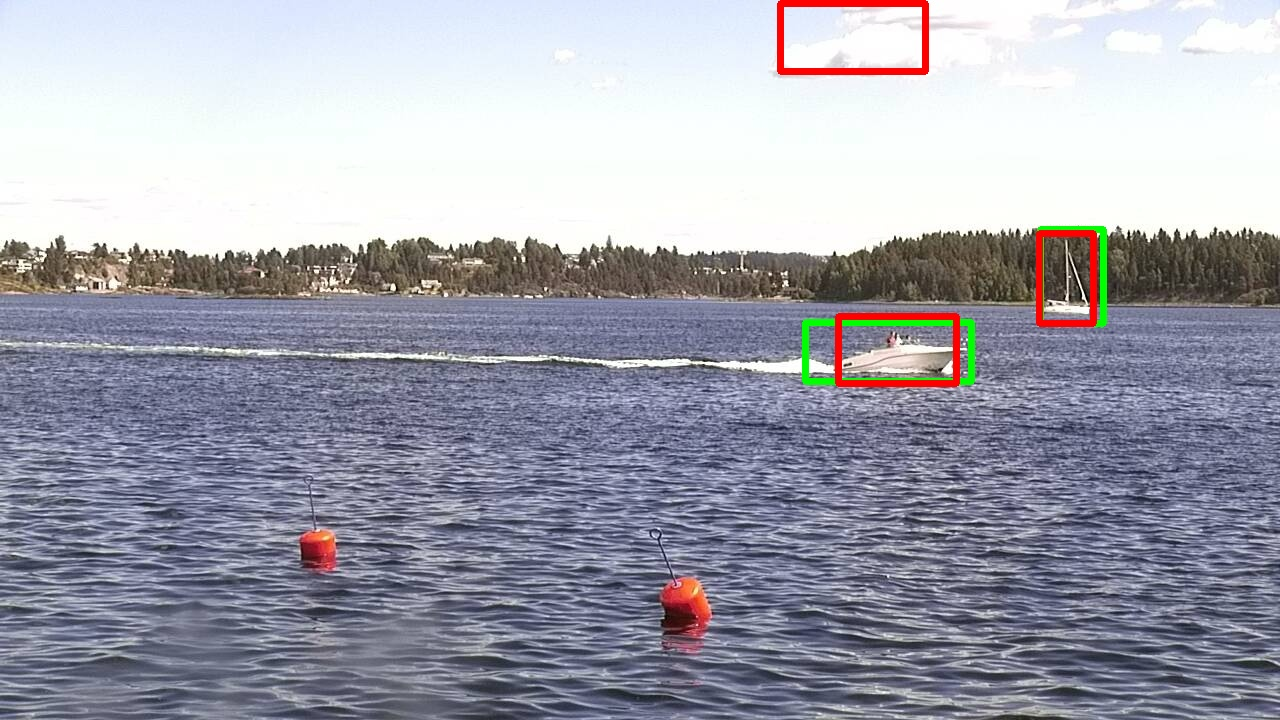
\includegraphics[width=0.9\linewidth]{results/case_buildings/yolo23/grove/yolo2/selected_06_25_frame0357.jpg}
  \caption{Yolo2}
  \label{fig:misclass_yolo2}
\end{subfigure}%
\begin{subfigure}{.5\textwidth}
  \centering
  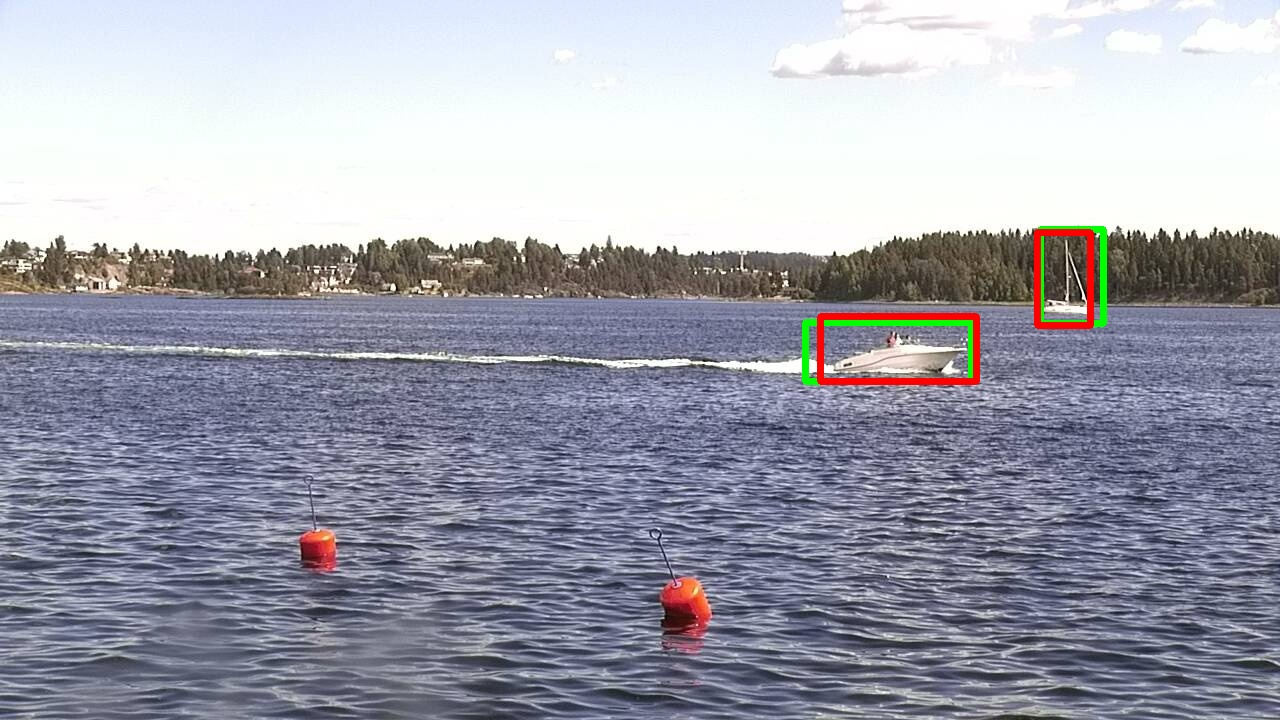
\includegraphics[width=.9\linewidth]{results/case_buildings/yolo23/grove/yolo3/selected_06_25_frame0357.jpg}
  \caption{Yolo3}
  \label{fig:misclass_yolo3}
\end{subfigure}
\caption{Yolo 2 misclassifies a cloud as a boat, Yolo3 does not. Red bounding boxes are detections, green bounding boxes are ground truth.}
\label{img:misclass_yolo}
\end{figure}

\newpage

\subsection{Tested on \textit{trf}}
\label{sec:test_on_trf}

The precision/recall curve for Yolo2, Yolo3, SSD2, and SSD3 on \textit{trf} can be seen in figure \ref{fig:trf_prec}. All the models perform very well on this dataset, where Yolo3 almost gets a perfect score with an average precision of 0.908, meaning it is very close to detect all the objects while having practically no misclassifications. This result could be an indication of overtraining on this dataset and will be discussed further in chapter \ref{dataset_divers}. 

\vspace{3mm}

Both the models trained on the building class, perform better than the model only trained on the boat class. As for the tests on \textit{bc} and \textit{bf} the differences between SSD2 and SSD3 are more evident than the differences between Yolo2 and Yolo3. The performance difference between SSD2 and SSD3 is also more significant than between Yolo2 and Yolo3, as can be seen in figure \ref{fig:trf_prec}


\begin{figure}[h!]
\begin{subfigure}{.5\textwidth}
  \centering
  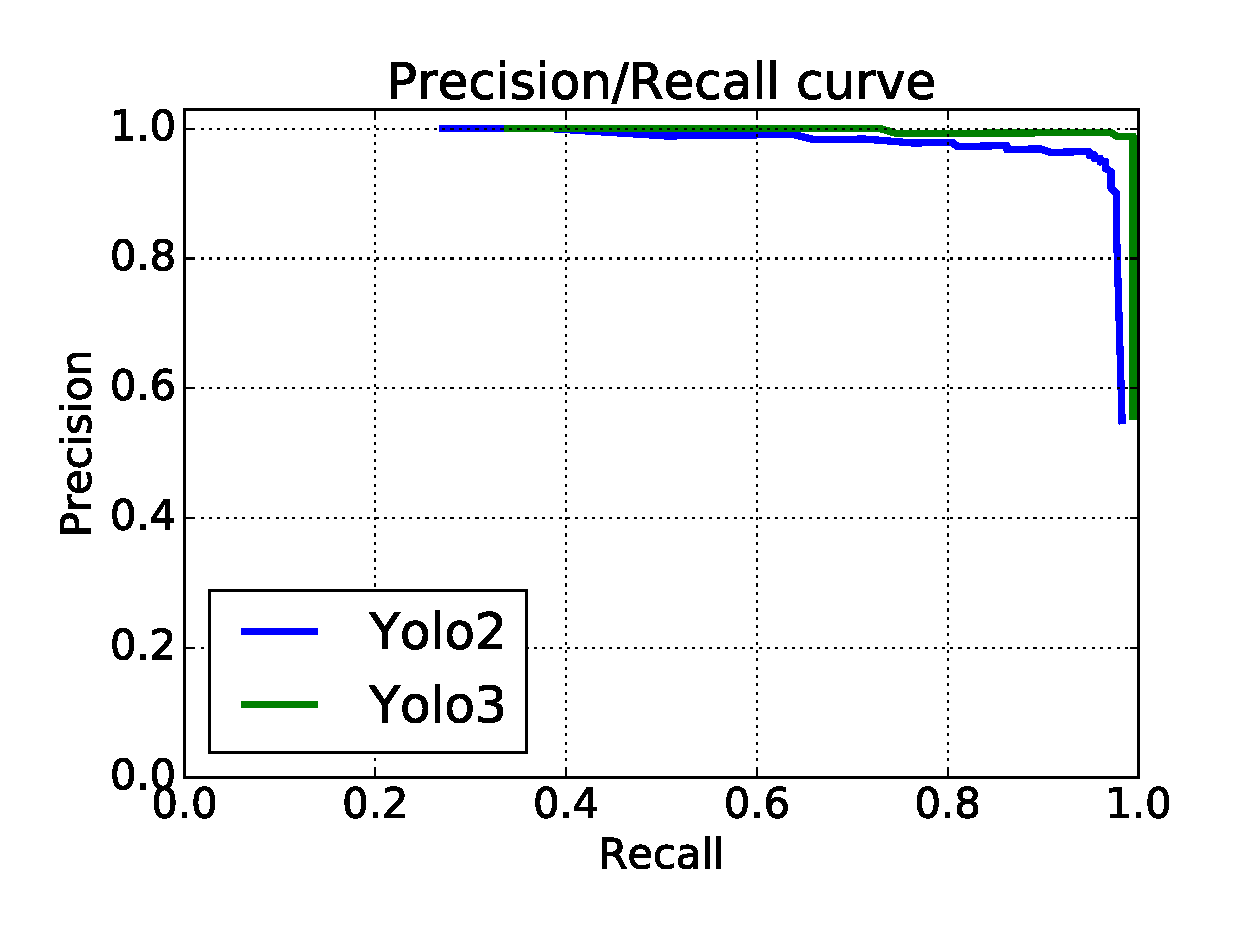
\includegraphics[width=0.8\linewidth]{results/case_buildings/prec_recall/yolo/trf.eps}
  \caption{Yolo tested on \textit{trf}}
  \label{fig:ex_trf_prec_rec_yolo}
\end{subfigure}%
\begin{subfigure}{.5\textwidth}
  \centering
  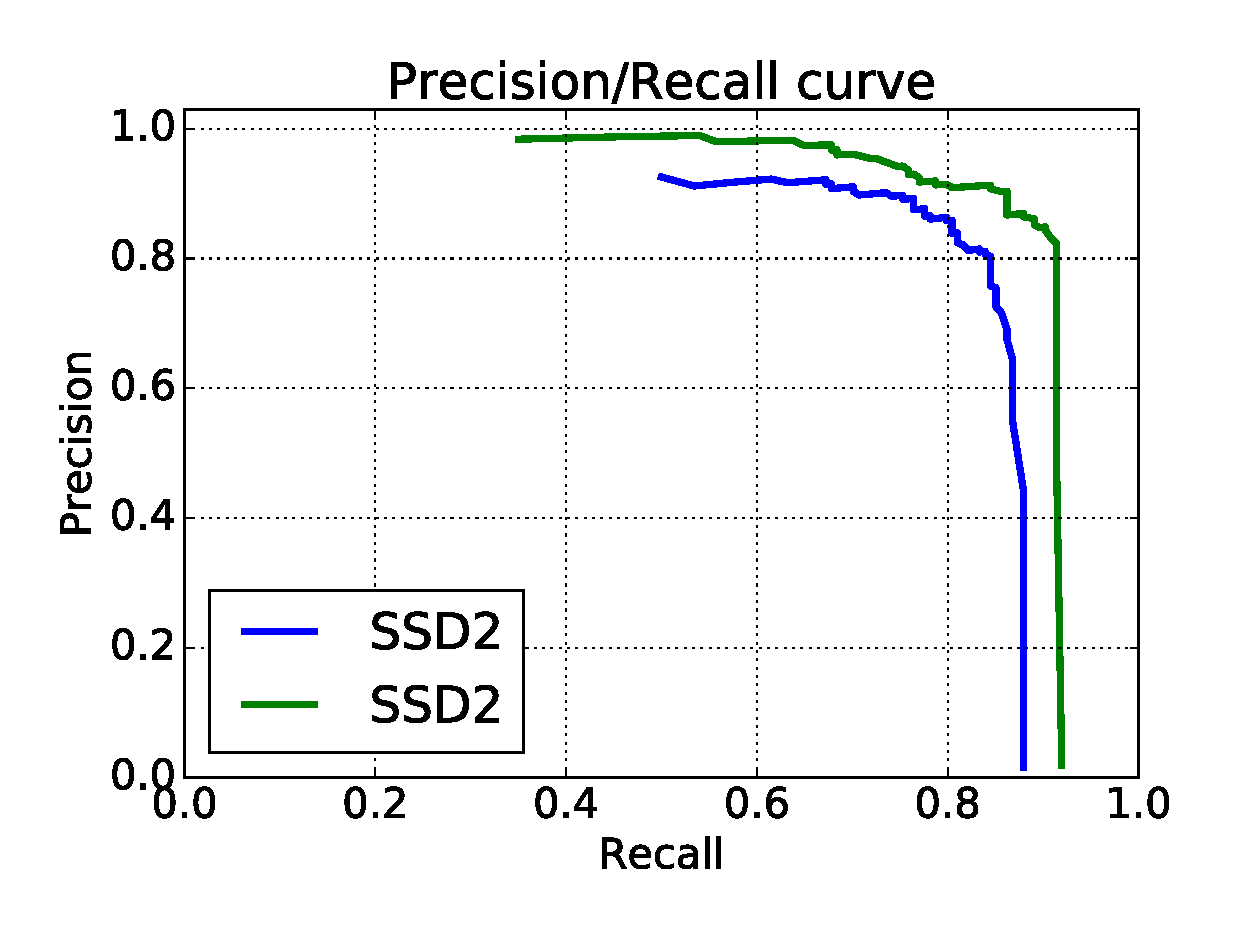
\includegraphics[width=.8\linewidth]{results/case_buildings/prec_recall/ssd/trf.eps}
  \caption{SSD tested on \textit{trf}}
  \label{fig:ex_trf_prec_rec_ssd}
\end{subfigure}
\caption{Precision/recall curves for Yolo2, Yolo3, SSD2 and SSD3 on \textit{trf}}
\label{fig:trf_prec}
\end{figure}

\subsubsection{SSD2 and SSD3 on \textit{trf}}

SSD2 has some of the same behaviors on \textit{trf} as it had on \textit{bc} and \textit{bf}. For instance, it sometimes classifies land as a boat, as shown in figure \ref{fig:ssd_trf_bigbox}. More examples of this behavior can be seen in Appendix C, chapter \ref{fig:ssd_trf_bigbox}.

\begin{figure}[h!]
\begin{subfigure}{.5\textwidth}
  \centering
  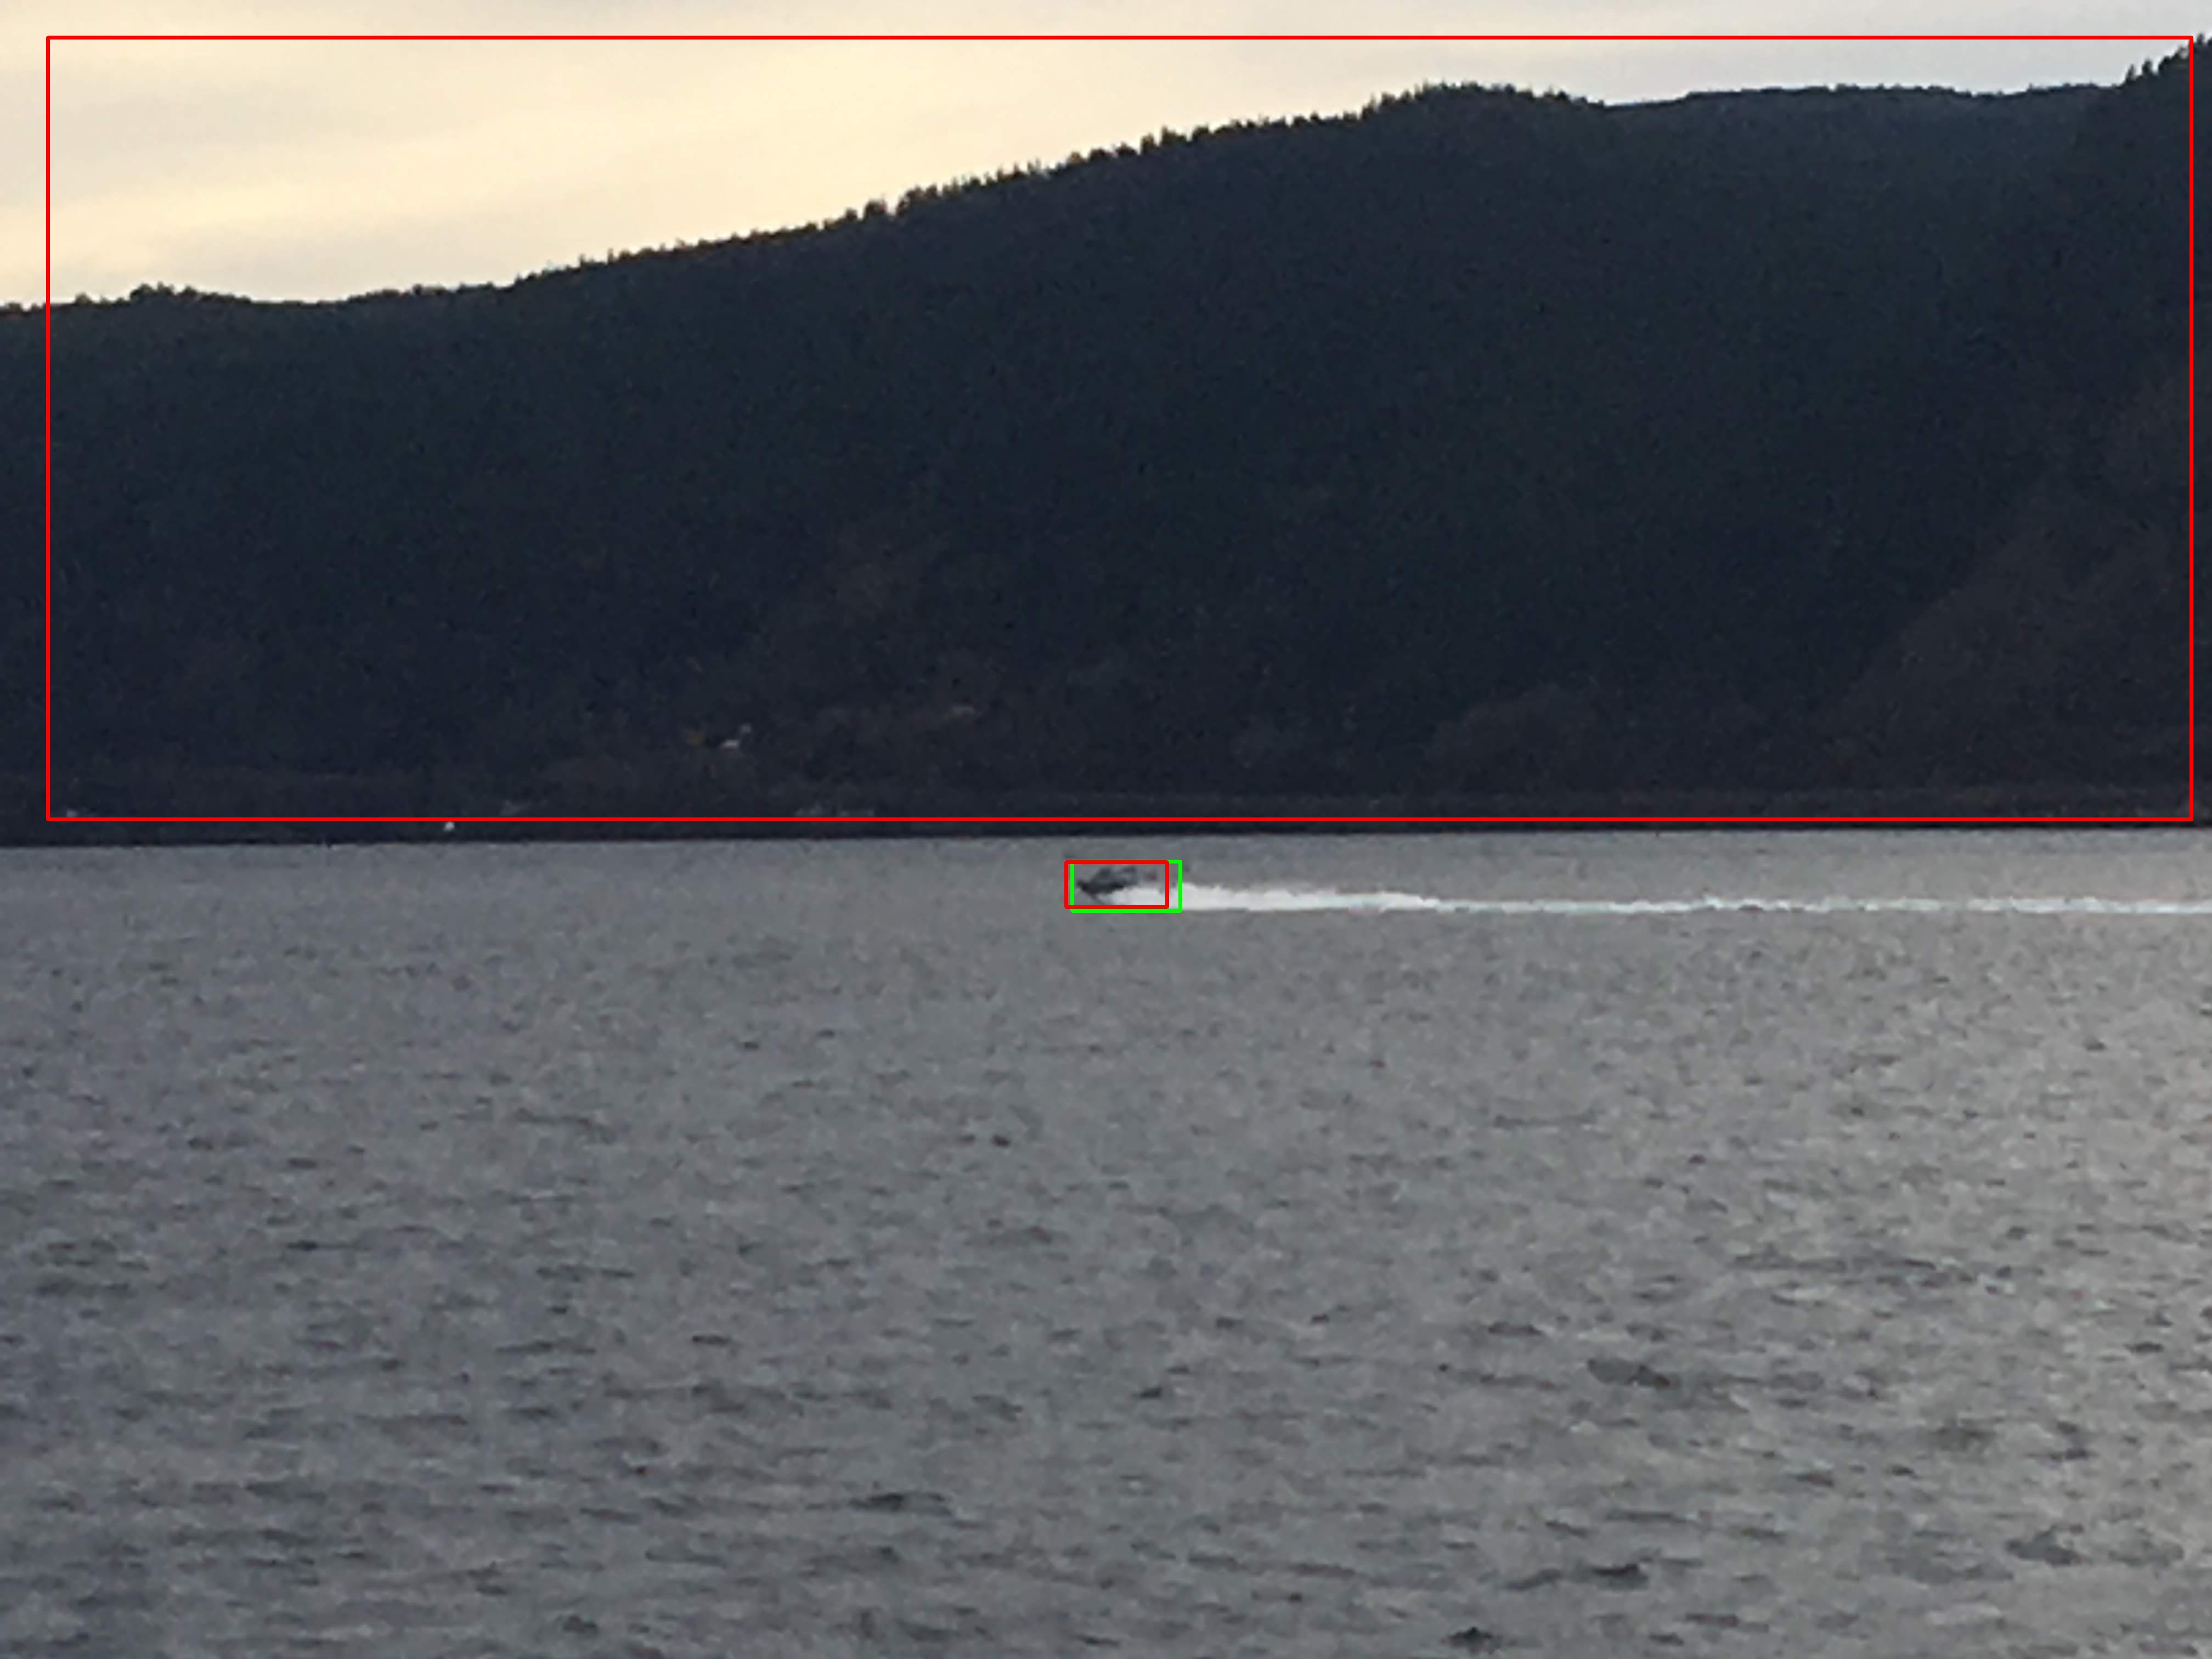
\includegraphics[width=0.8\linewidth]{results/case_buildings/ssdtrf/ssd2/grov2/IMG_2325.jpg}
  \caption{SSD2}
  \label{fig:ex_trf_prec_rec_yolo}
\end{subfigure}%
\begin{subfigure}{.5\textwidth}
  \centering
  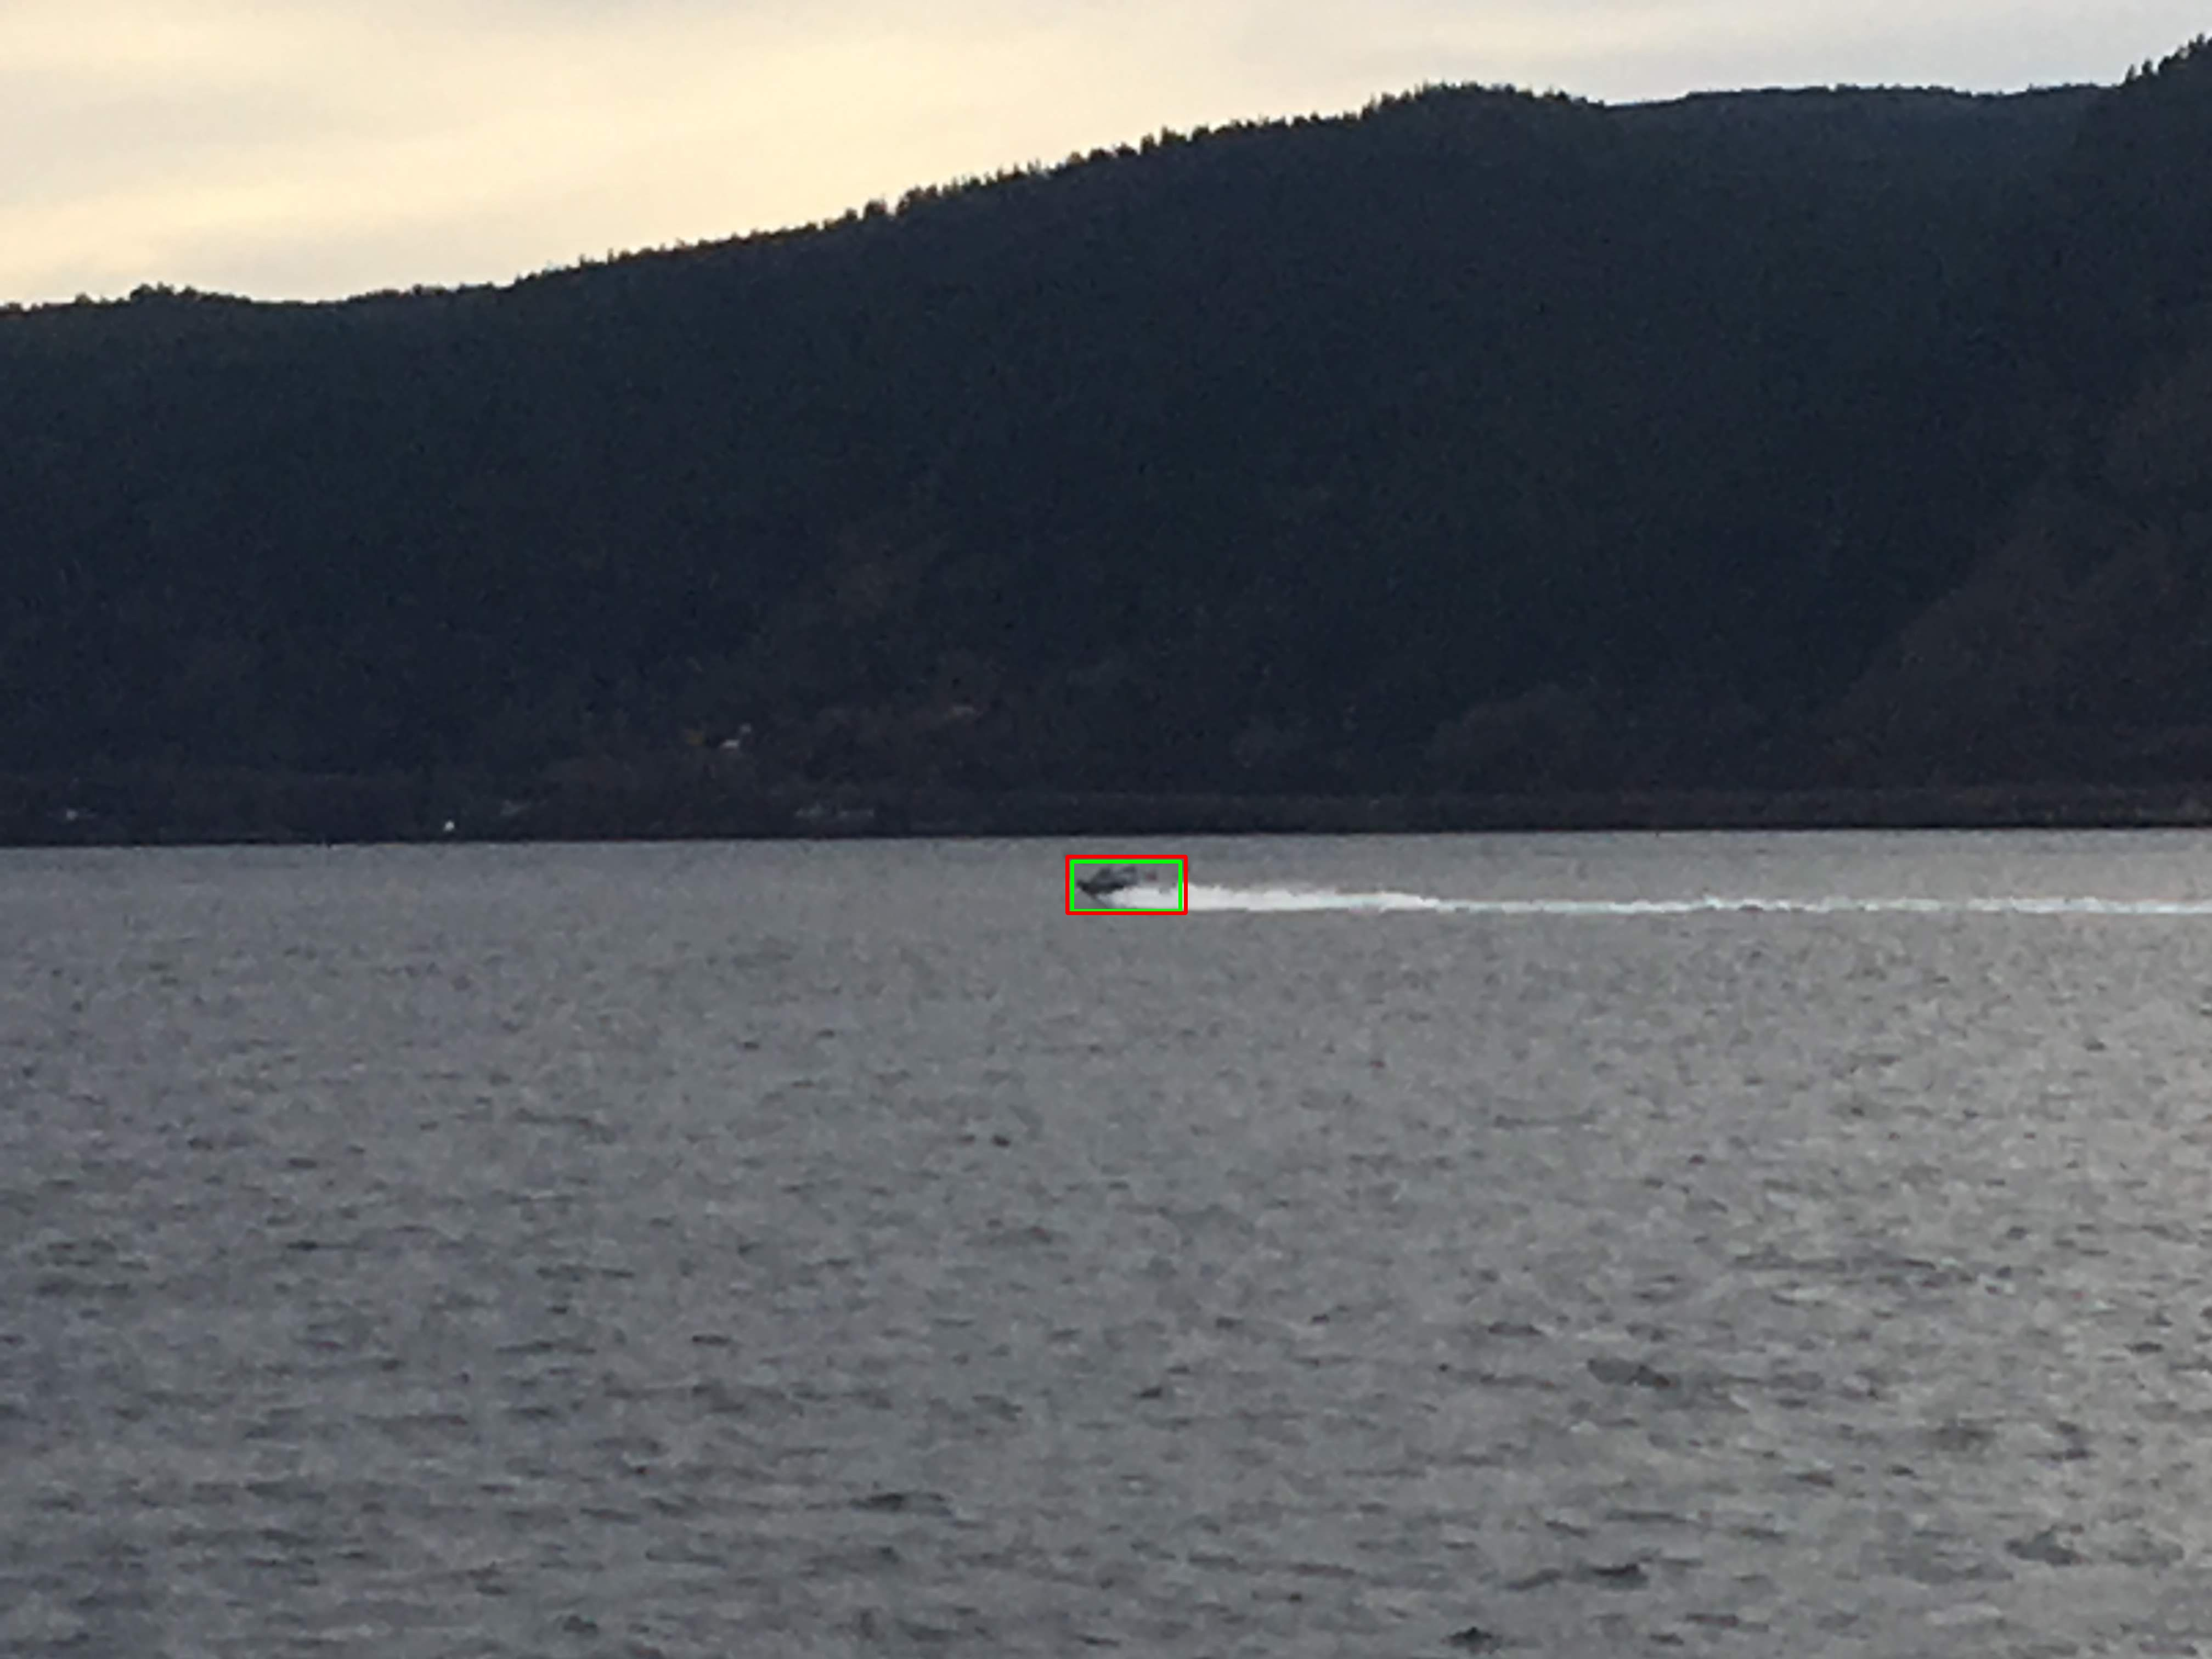
\includegraphics[width=.8\linewidth]{results/case_buildings/ssdtrf/ssd3/grov2/IMG_2325.jpg}
  \caption{SSD3}
  \label{fig:ex_trf_prec_rec_ssd}
\end{subfigure}
\caption{SSD2 and SSD3 example image}
\label{fig:ssd_trf_bigbox}
\end{figure}

There are examples where SSD2 detects boats correctly while SSD3 don't and vice versa. For example images of this behaviour see Appendix C, chapter \ref{sec_ssd3_better_trf} and \ref{sec_ssd2_better_trf}. In a few test images, SSD3 wrongly classifies buildings as boats, while SSD2 does not. This is counter-intuitive since the idea behind training SSD3 on buildings was to make it suppress these detections. An example of this is shown in figure \ref{fig:ssd3_misclassify}.

\begin{figure}[h!]
\begin{subfigure}{.5\textwidth}
  \centering
  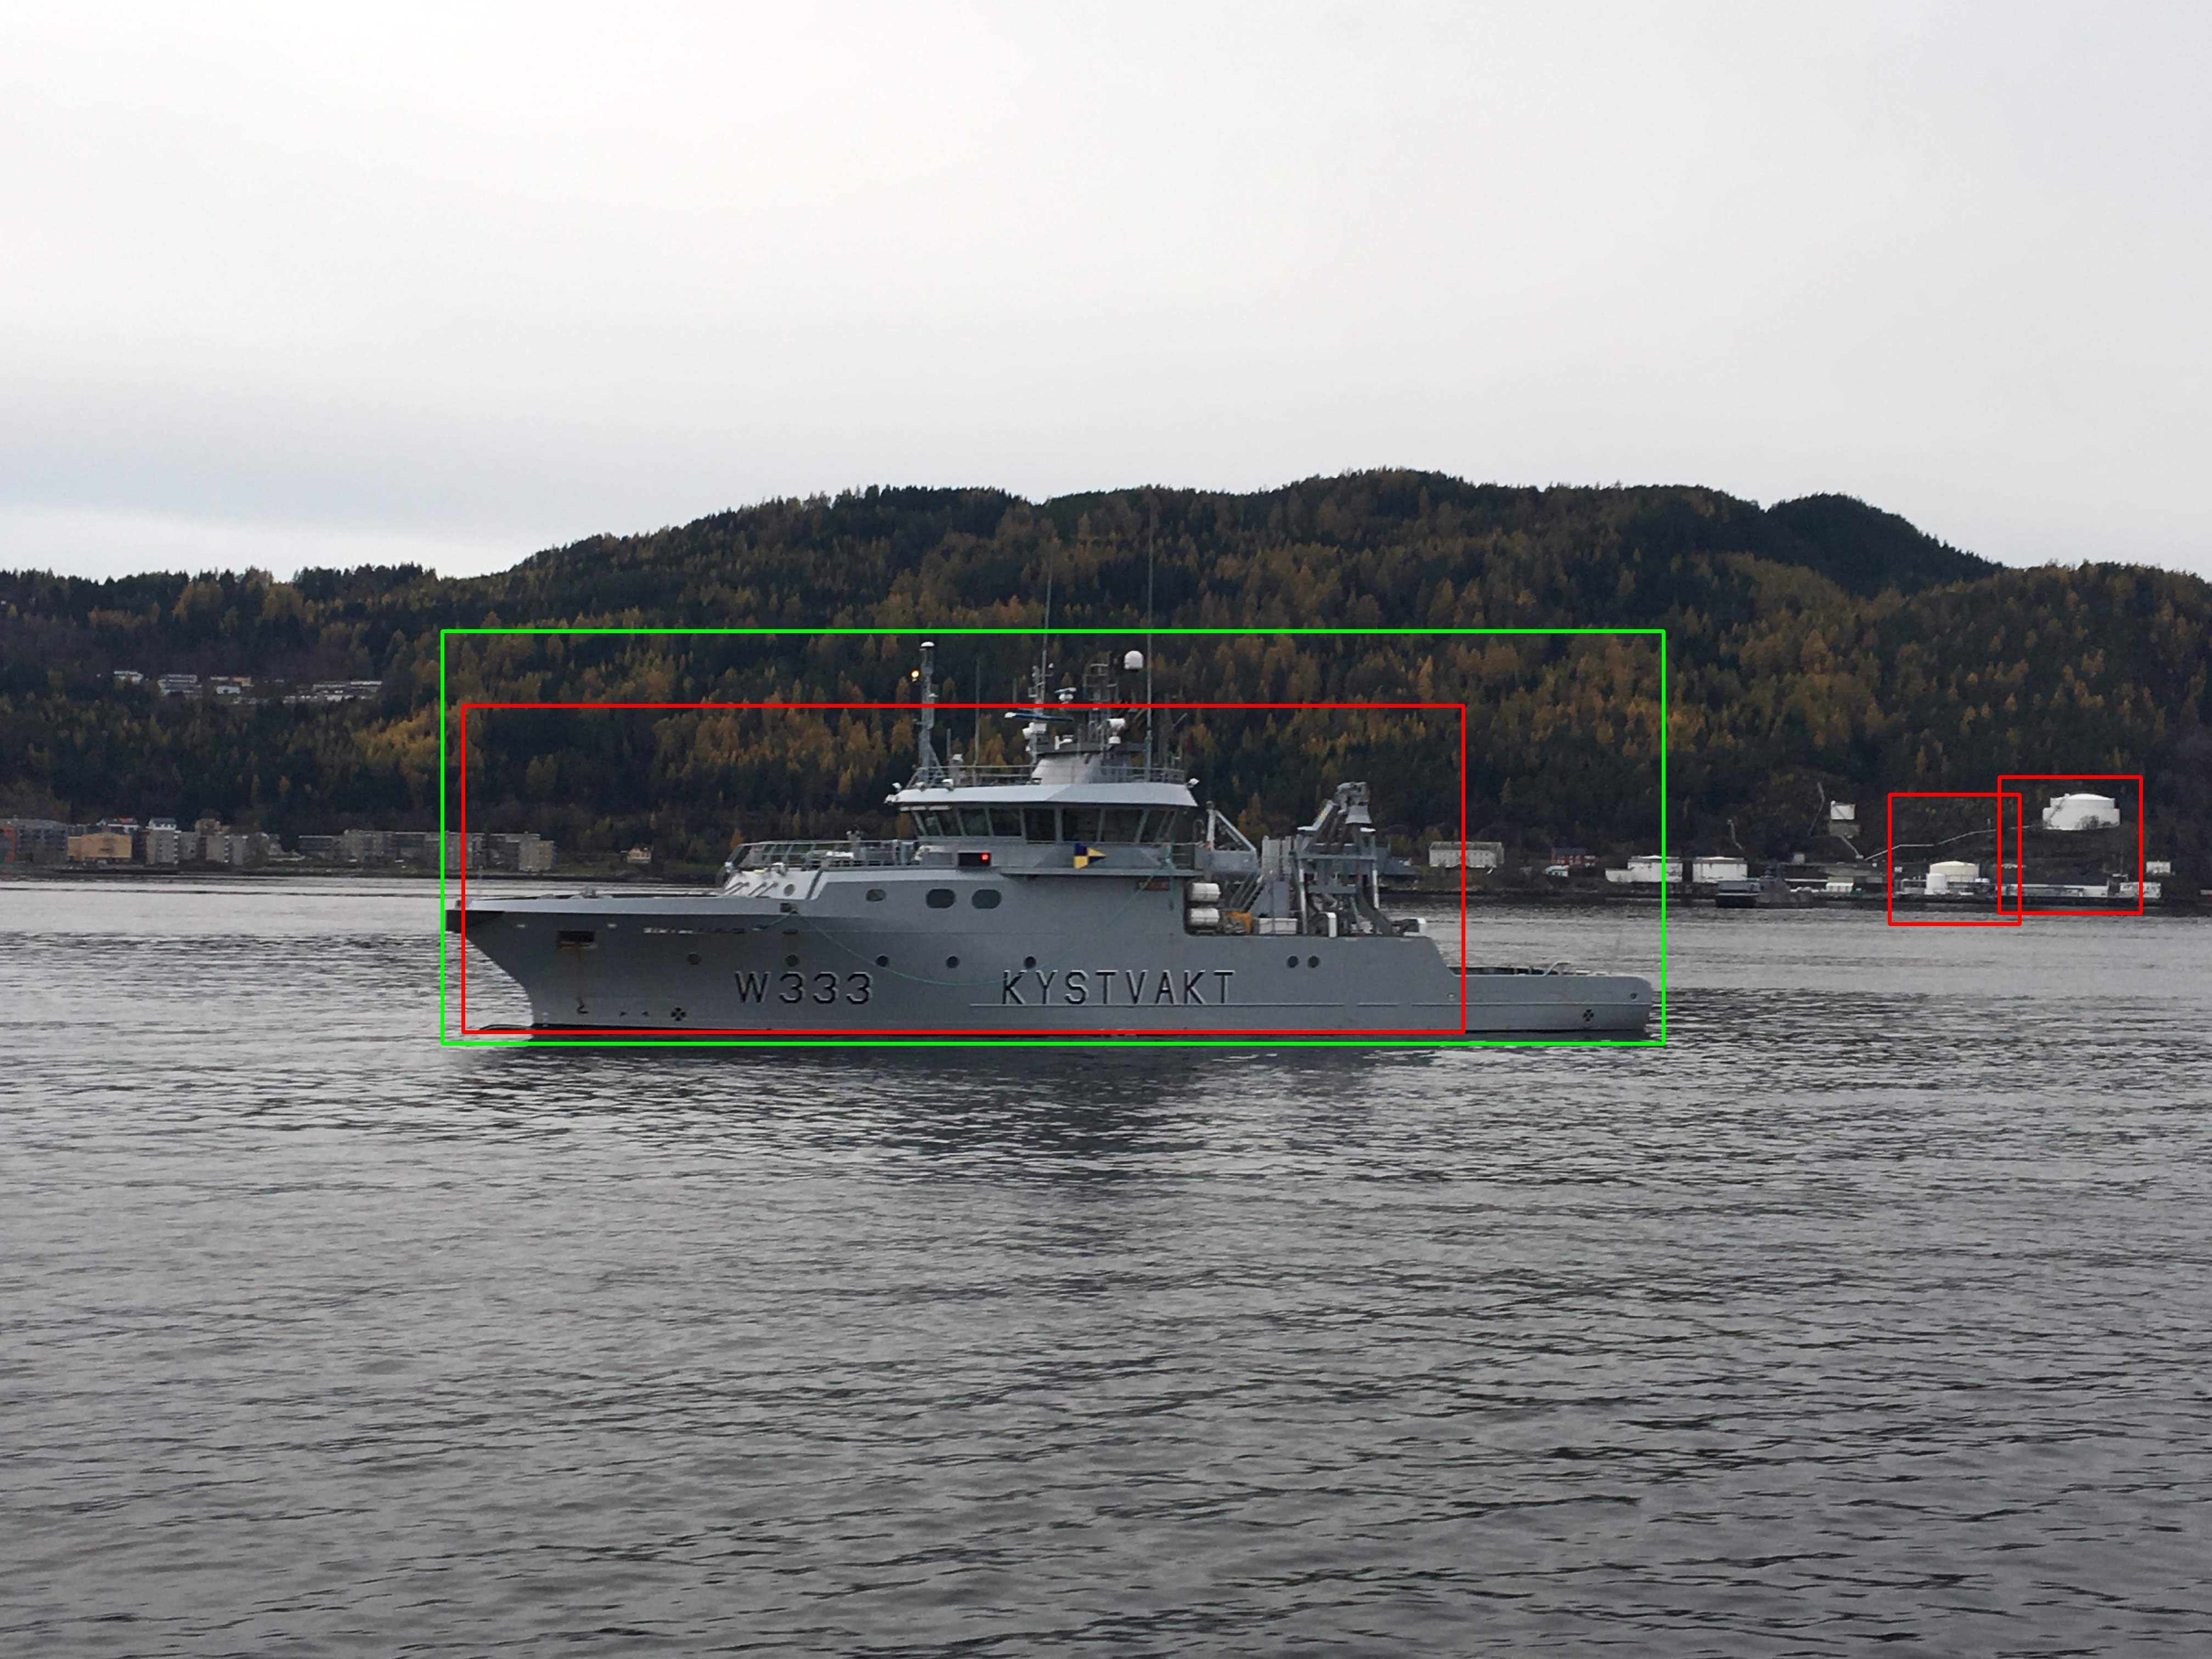
\includegraphics[width=0.8\linewidth]{results/case_buildings/ssdtrf/ssd2/grov3/IMG_2680.jpg}
  \caption{SSD2}
  \label{fig:ex_trf_prec_rec_yolo}
\end{subfigure}%
\begin{subfigure}{.5\textwidth}
  \centering
  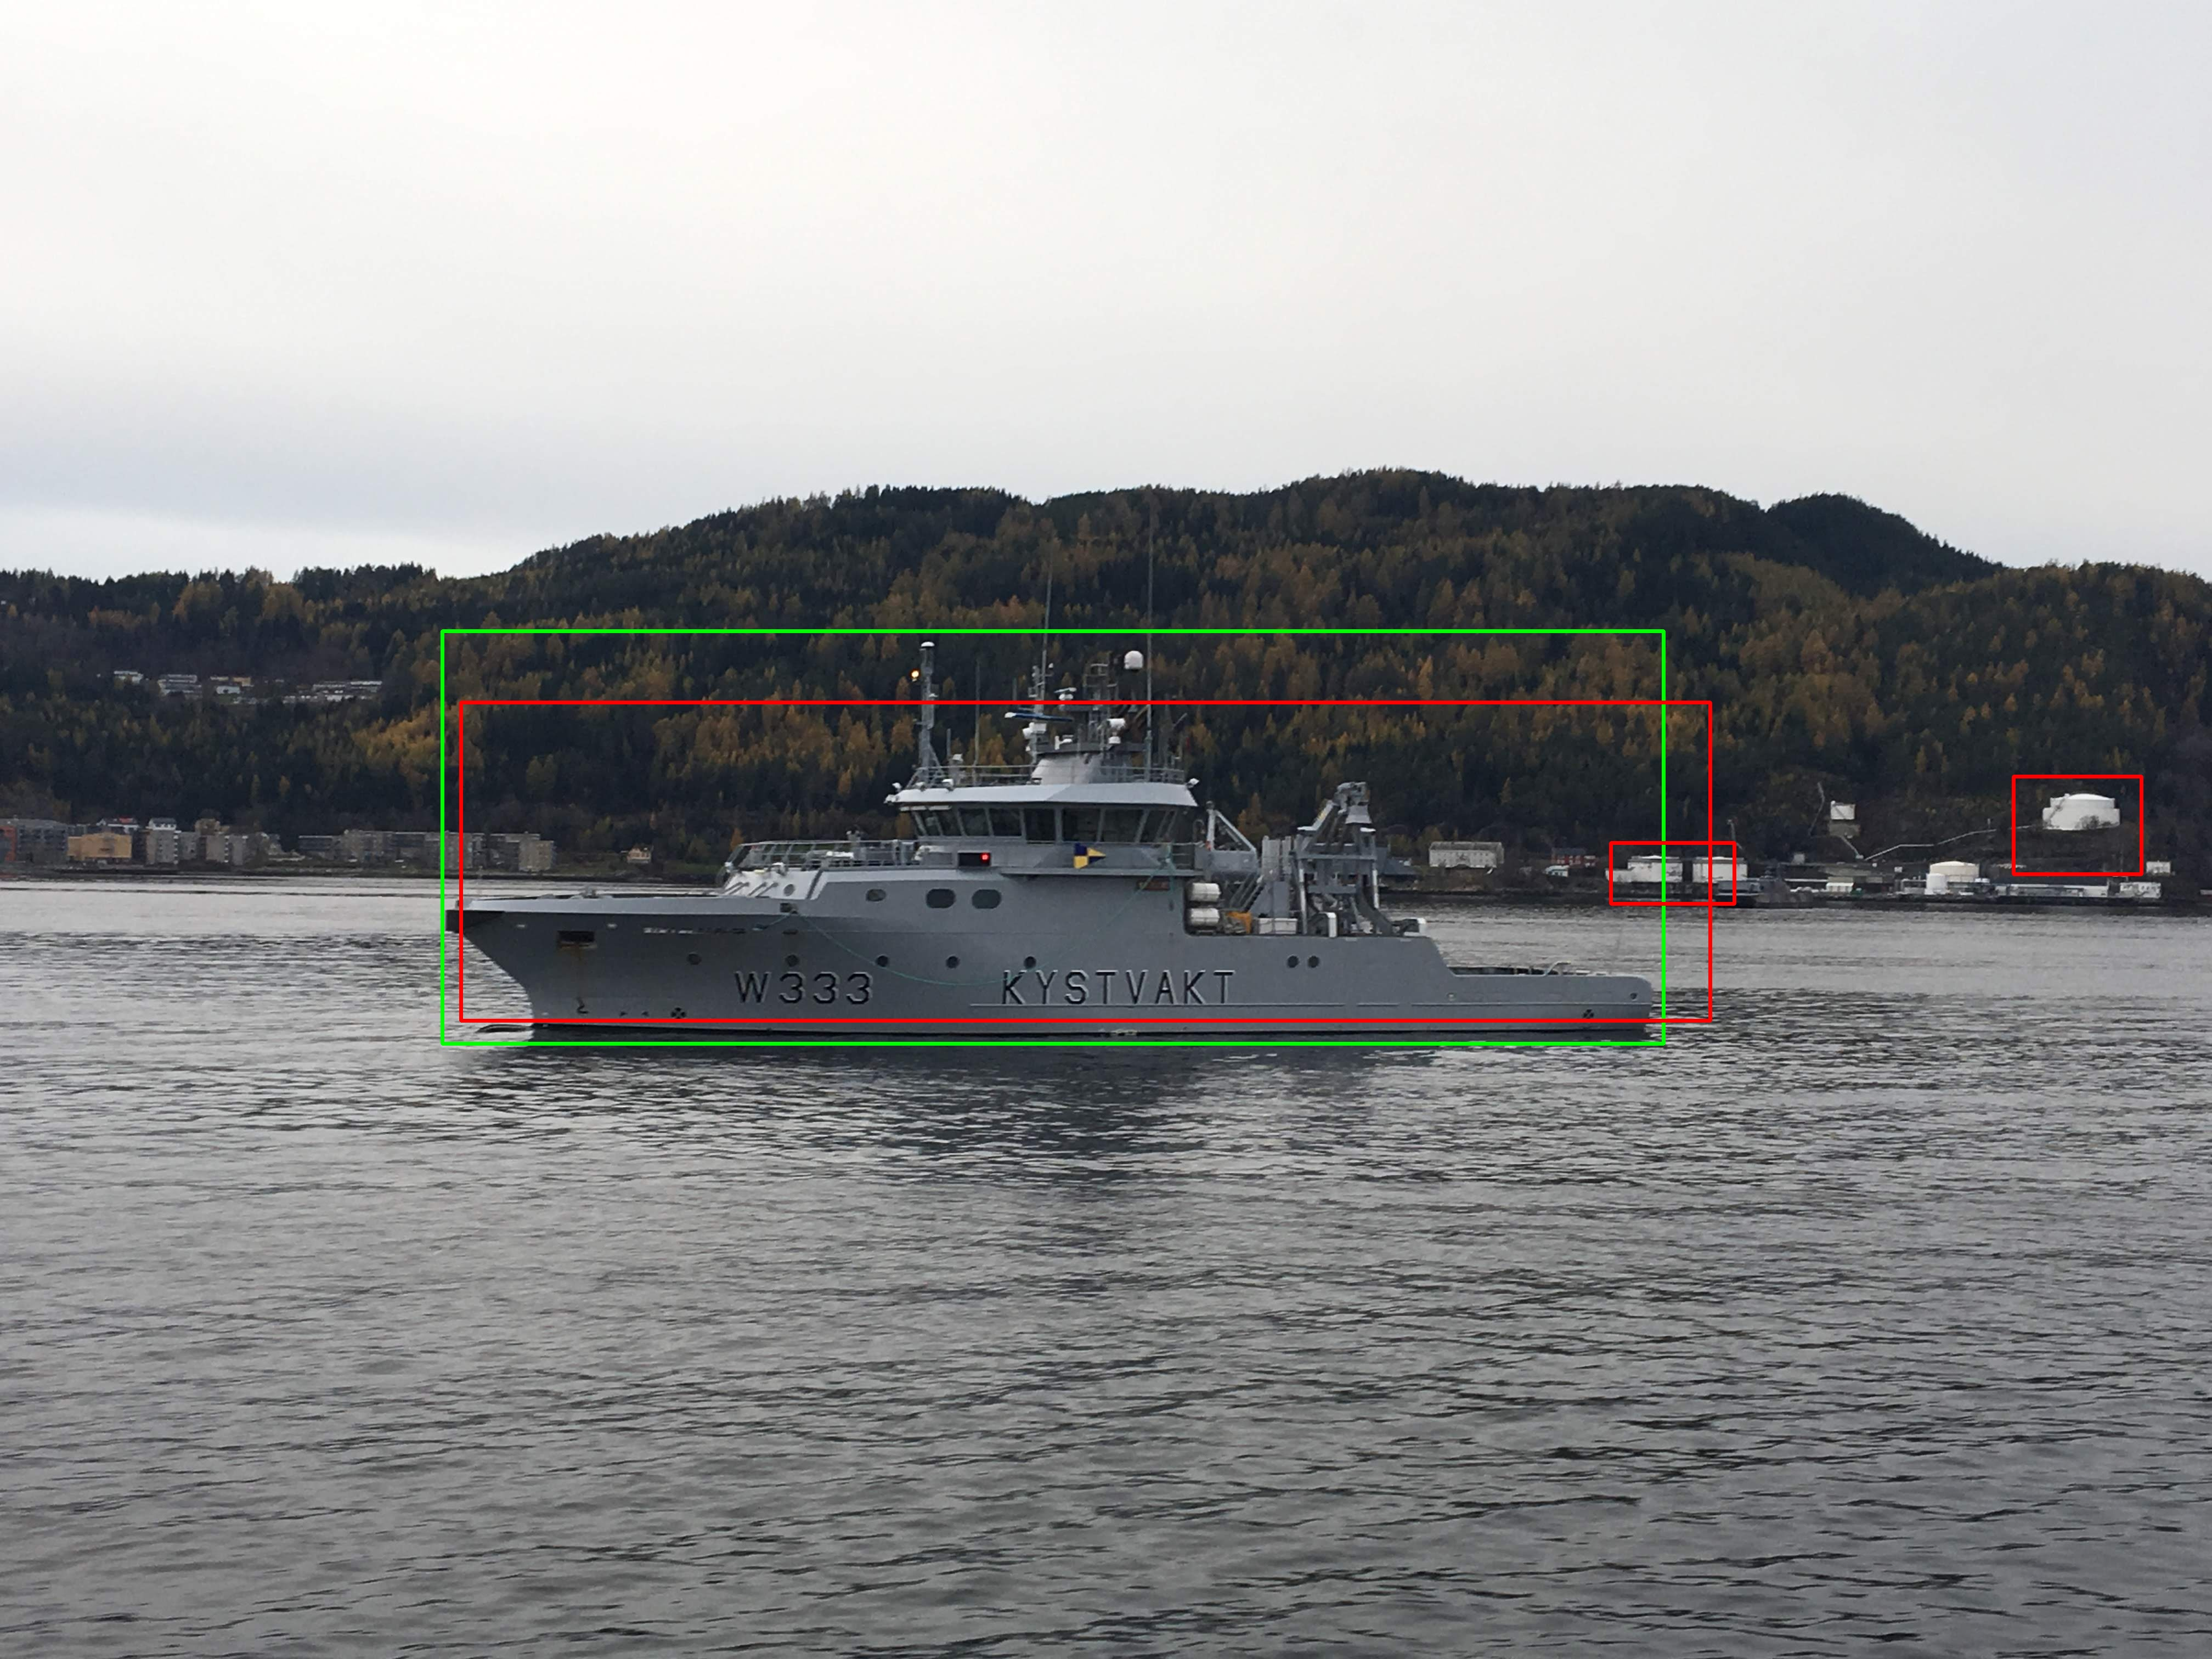
\includegraphics[width=.8\linewidth]{results/case_buildings/ssdtrf/ssd3/grov3/IMG_2680.jpg}
  \caption{SSD3}
  \label{fig:ex_trf_prec_rec_ssd}
\end{subfigure}
\caption{SSD3 misclassifies two buildings as boats}
\label{fig:ssd3_misclassify}
\end{figure}

In this figure \ref{fig:ssd3_misclassify} SSD3 does not detect the buildings as buildings, this will be discussed further in chapter \ref{sec:build_trf}.

\vspace{3mm}

\subsubsection{Yolo2 and Yolo3 on \textit{trf}}

Yolo2 and Yolo3 both have outstanding results on \textit{trf}, but Yolo2 has a few misclassifications that Yolo3 does not have. In figure \ref{fig:yolo2_misclassify} Yolo2 detects land as a boat, and in figure \ref{fig:Yolo3_better_trf} Yolo3 detects a boat that Yolo2 does not. There are not many examples where their performance differs much, but there are a few which makes Yolo3 a little more robust than Yolo2.

\begin{figure}[h!]
\begin{subfigure}{.5\textwidth}
  \centering
  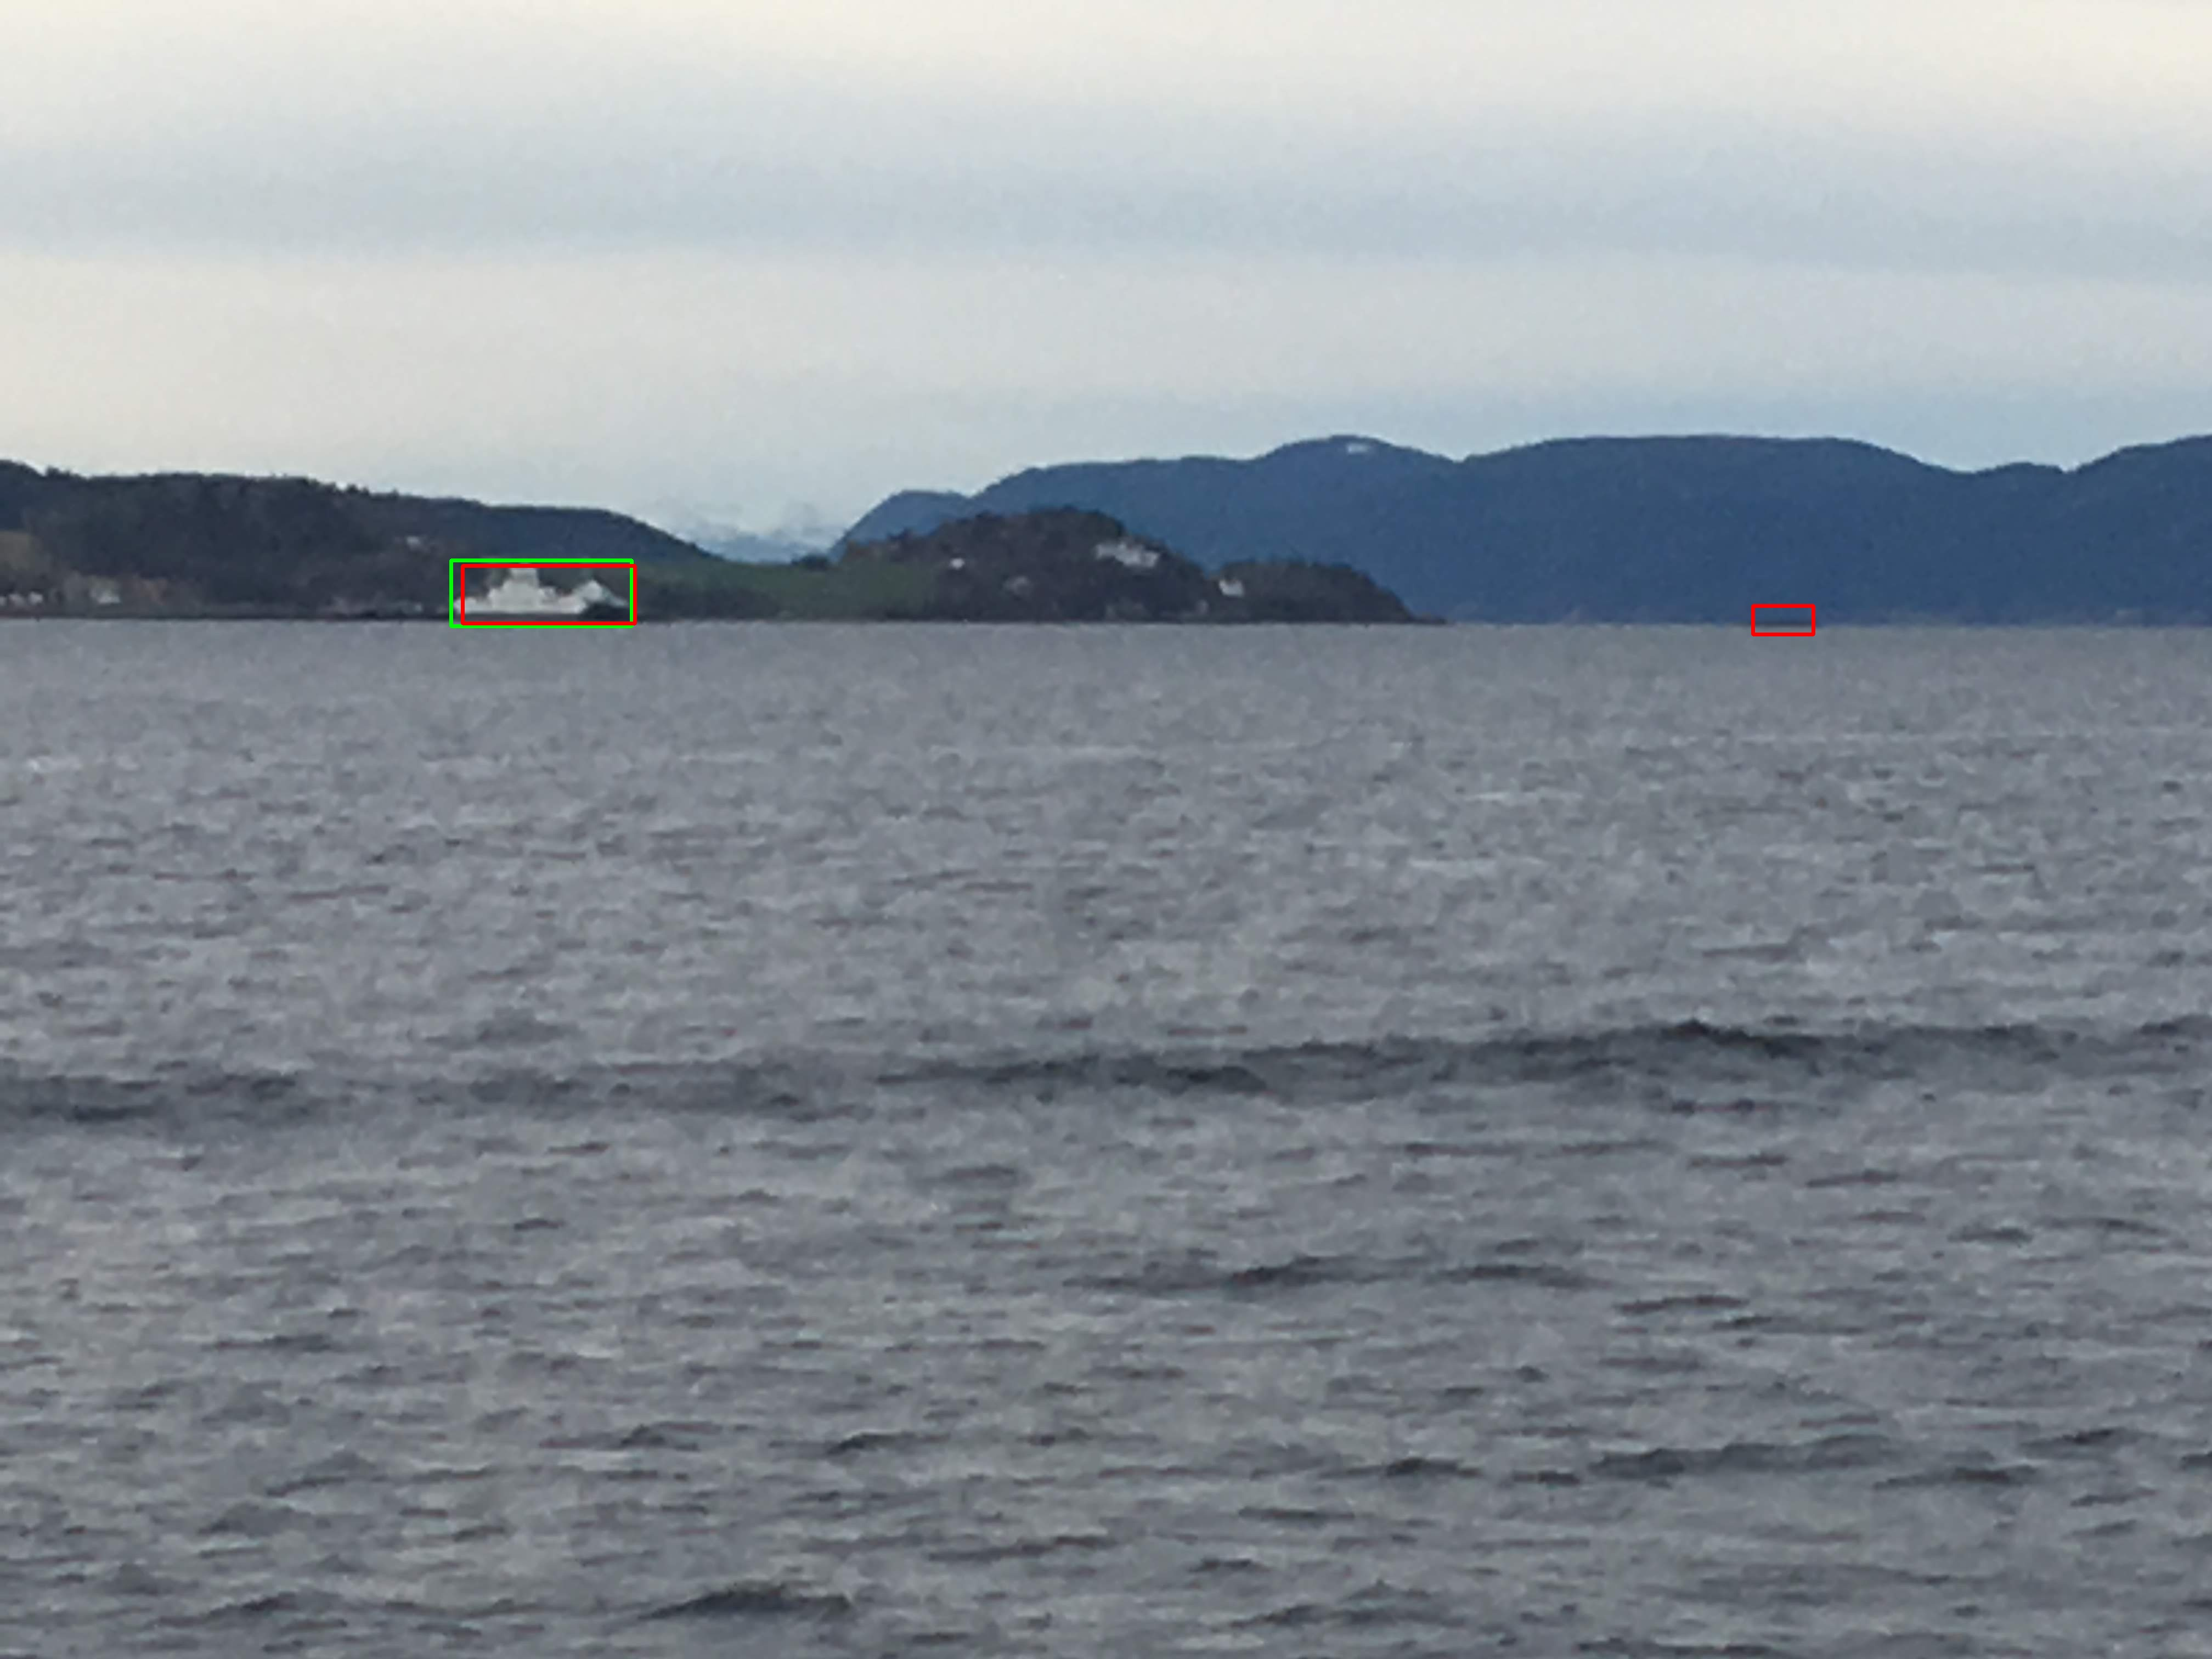
\includegraphics[width=0.8\linewidth]{results/case_buildings/yolotrf/Yolo2/IMG_2300.jpg}
  \caption{Yolo2}
  %\label{fig:ex_trf_prec_rec_yolo}
\end{subfigure}%
\begin{subfigure}{.5\textwidth}
  \centering
  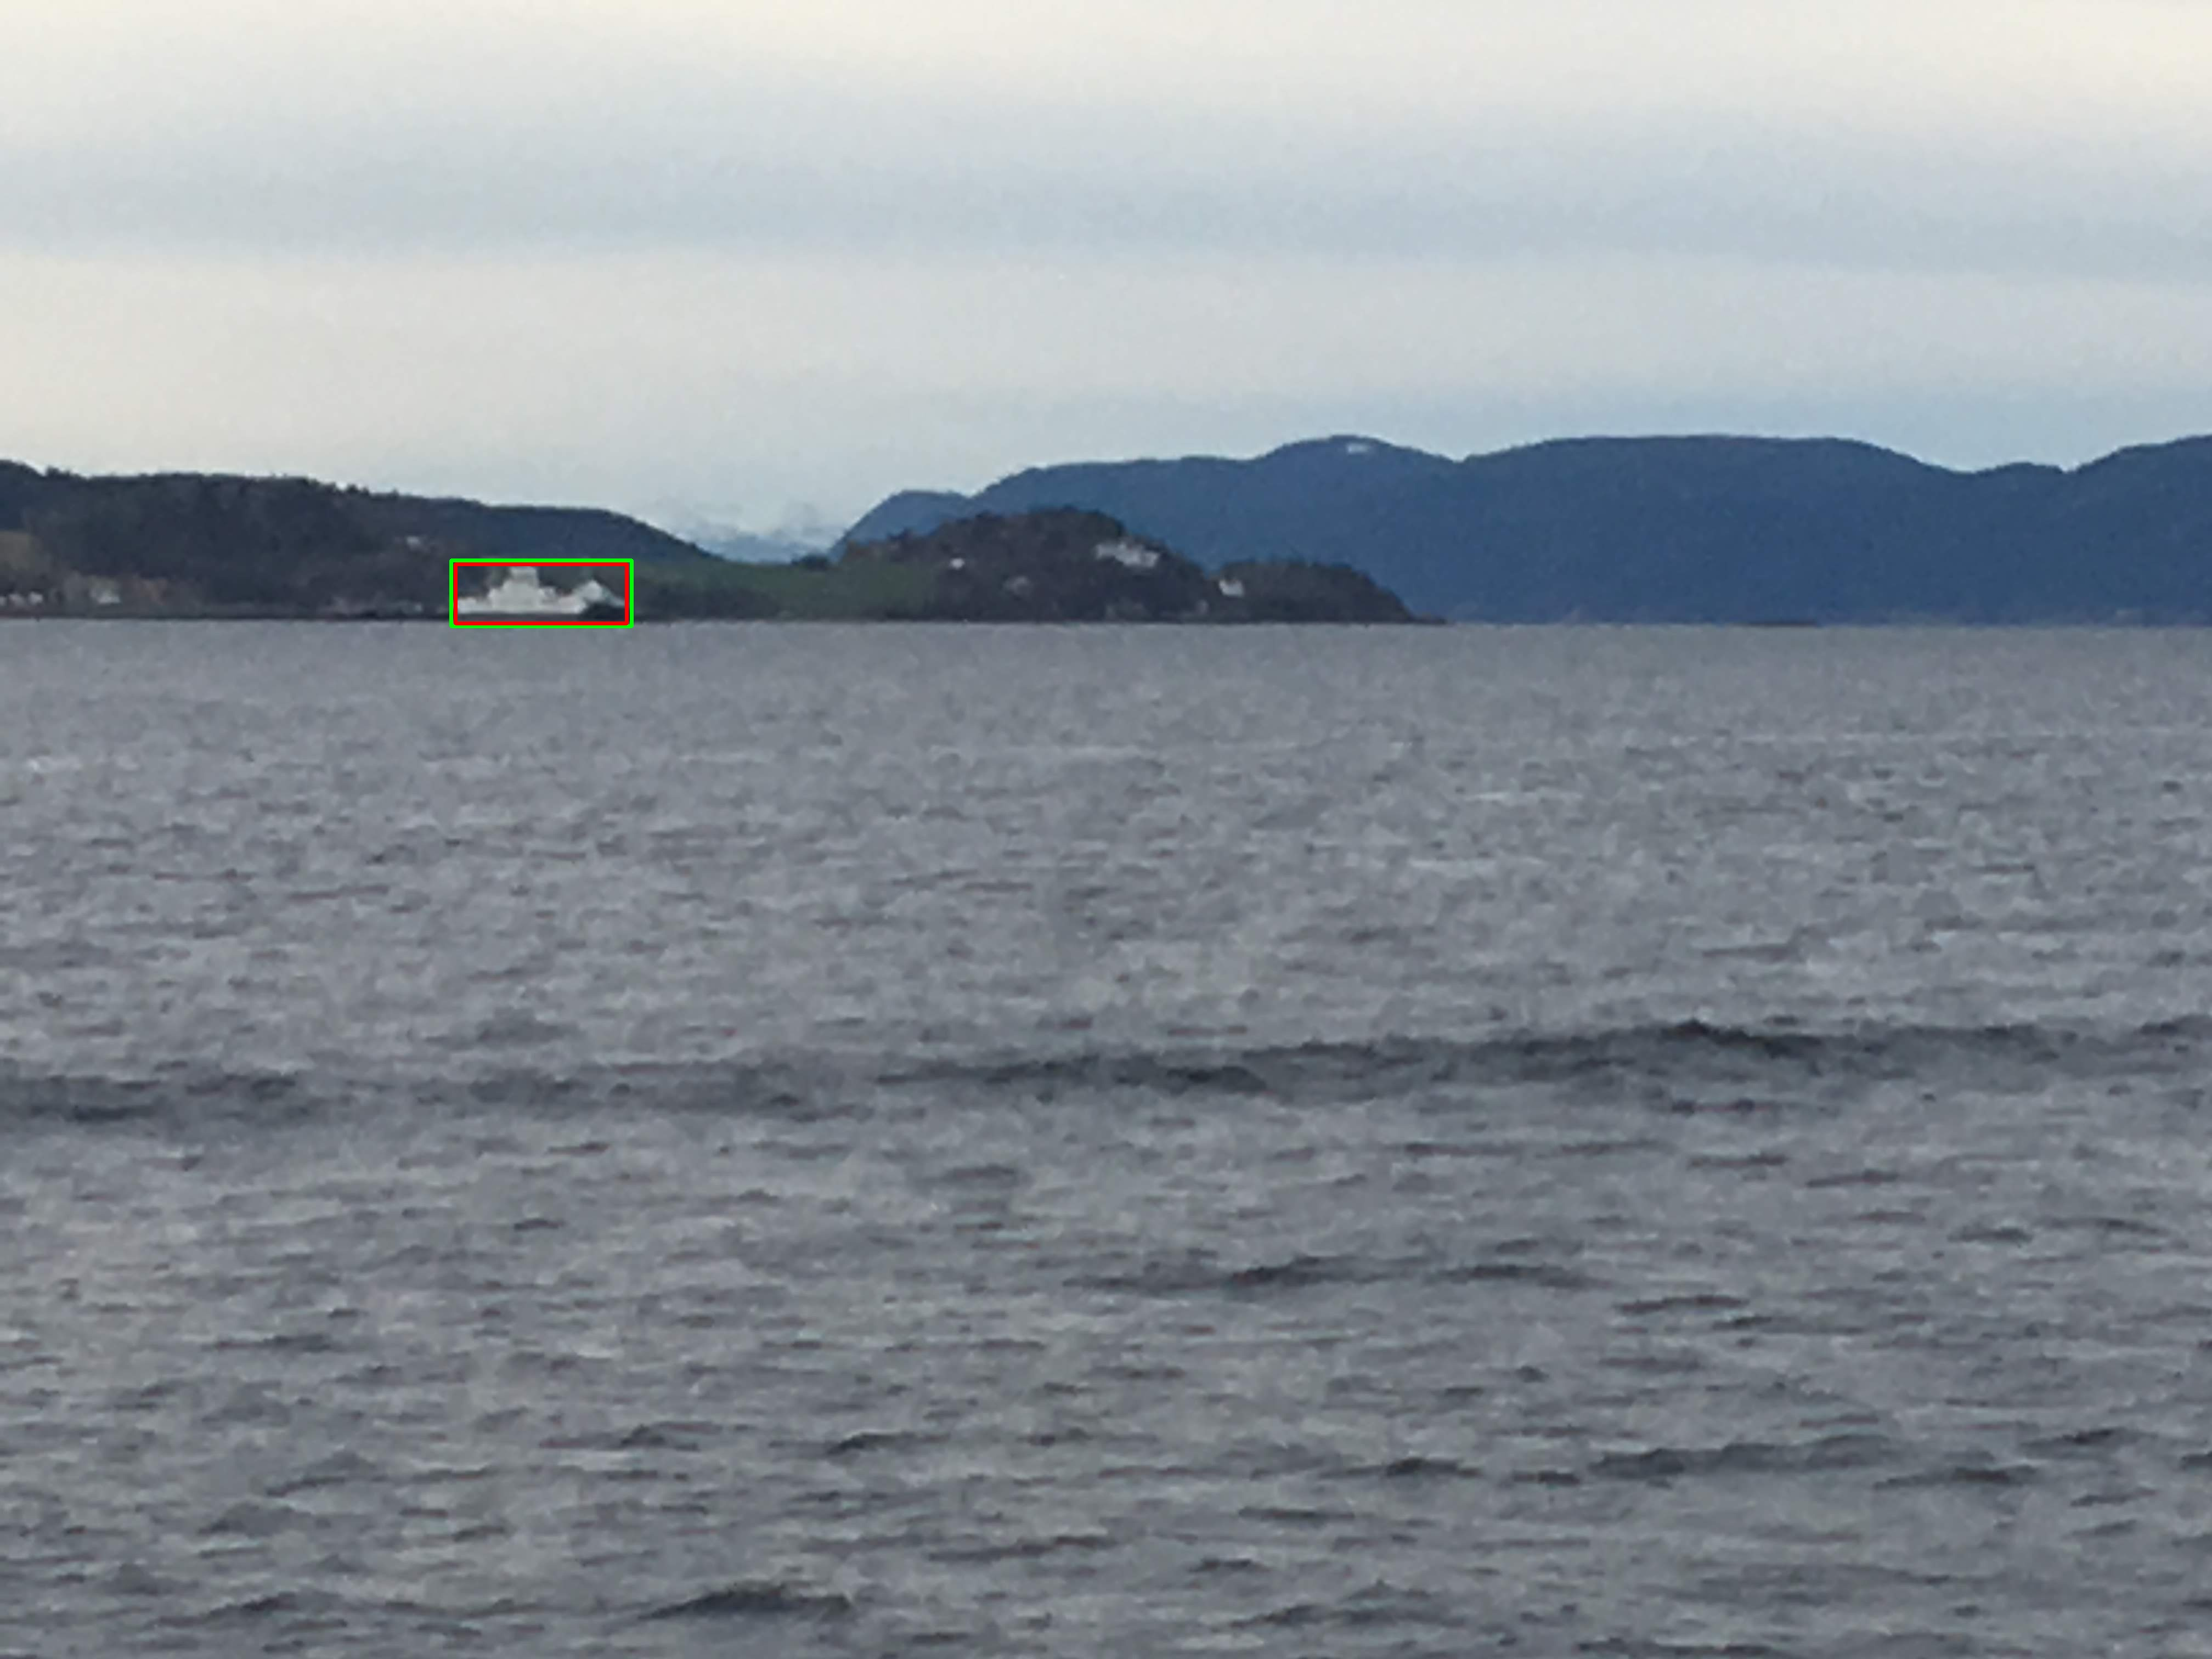
\includegraphics[width=.8\linewidth]{results/case_buildings/yolotrf/Yolo3/IMG_2300.jpg}
  \caption{Yolo3}
  %\label{fig:ex_trf_prec_rec_ssd}
\end{subfigure}
\caption{Yolo2 misclassifies land as boat}
\label{fig:yolo2_misclassify}
\end{figure}

\begin{figure}[h!]
\begin{subfigure}{.5\textwidth}
  \centering
  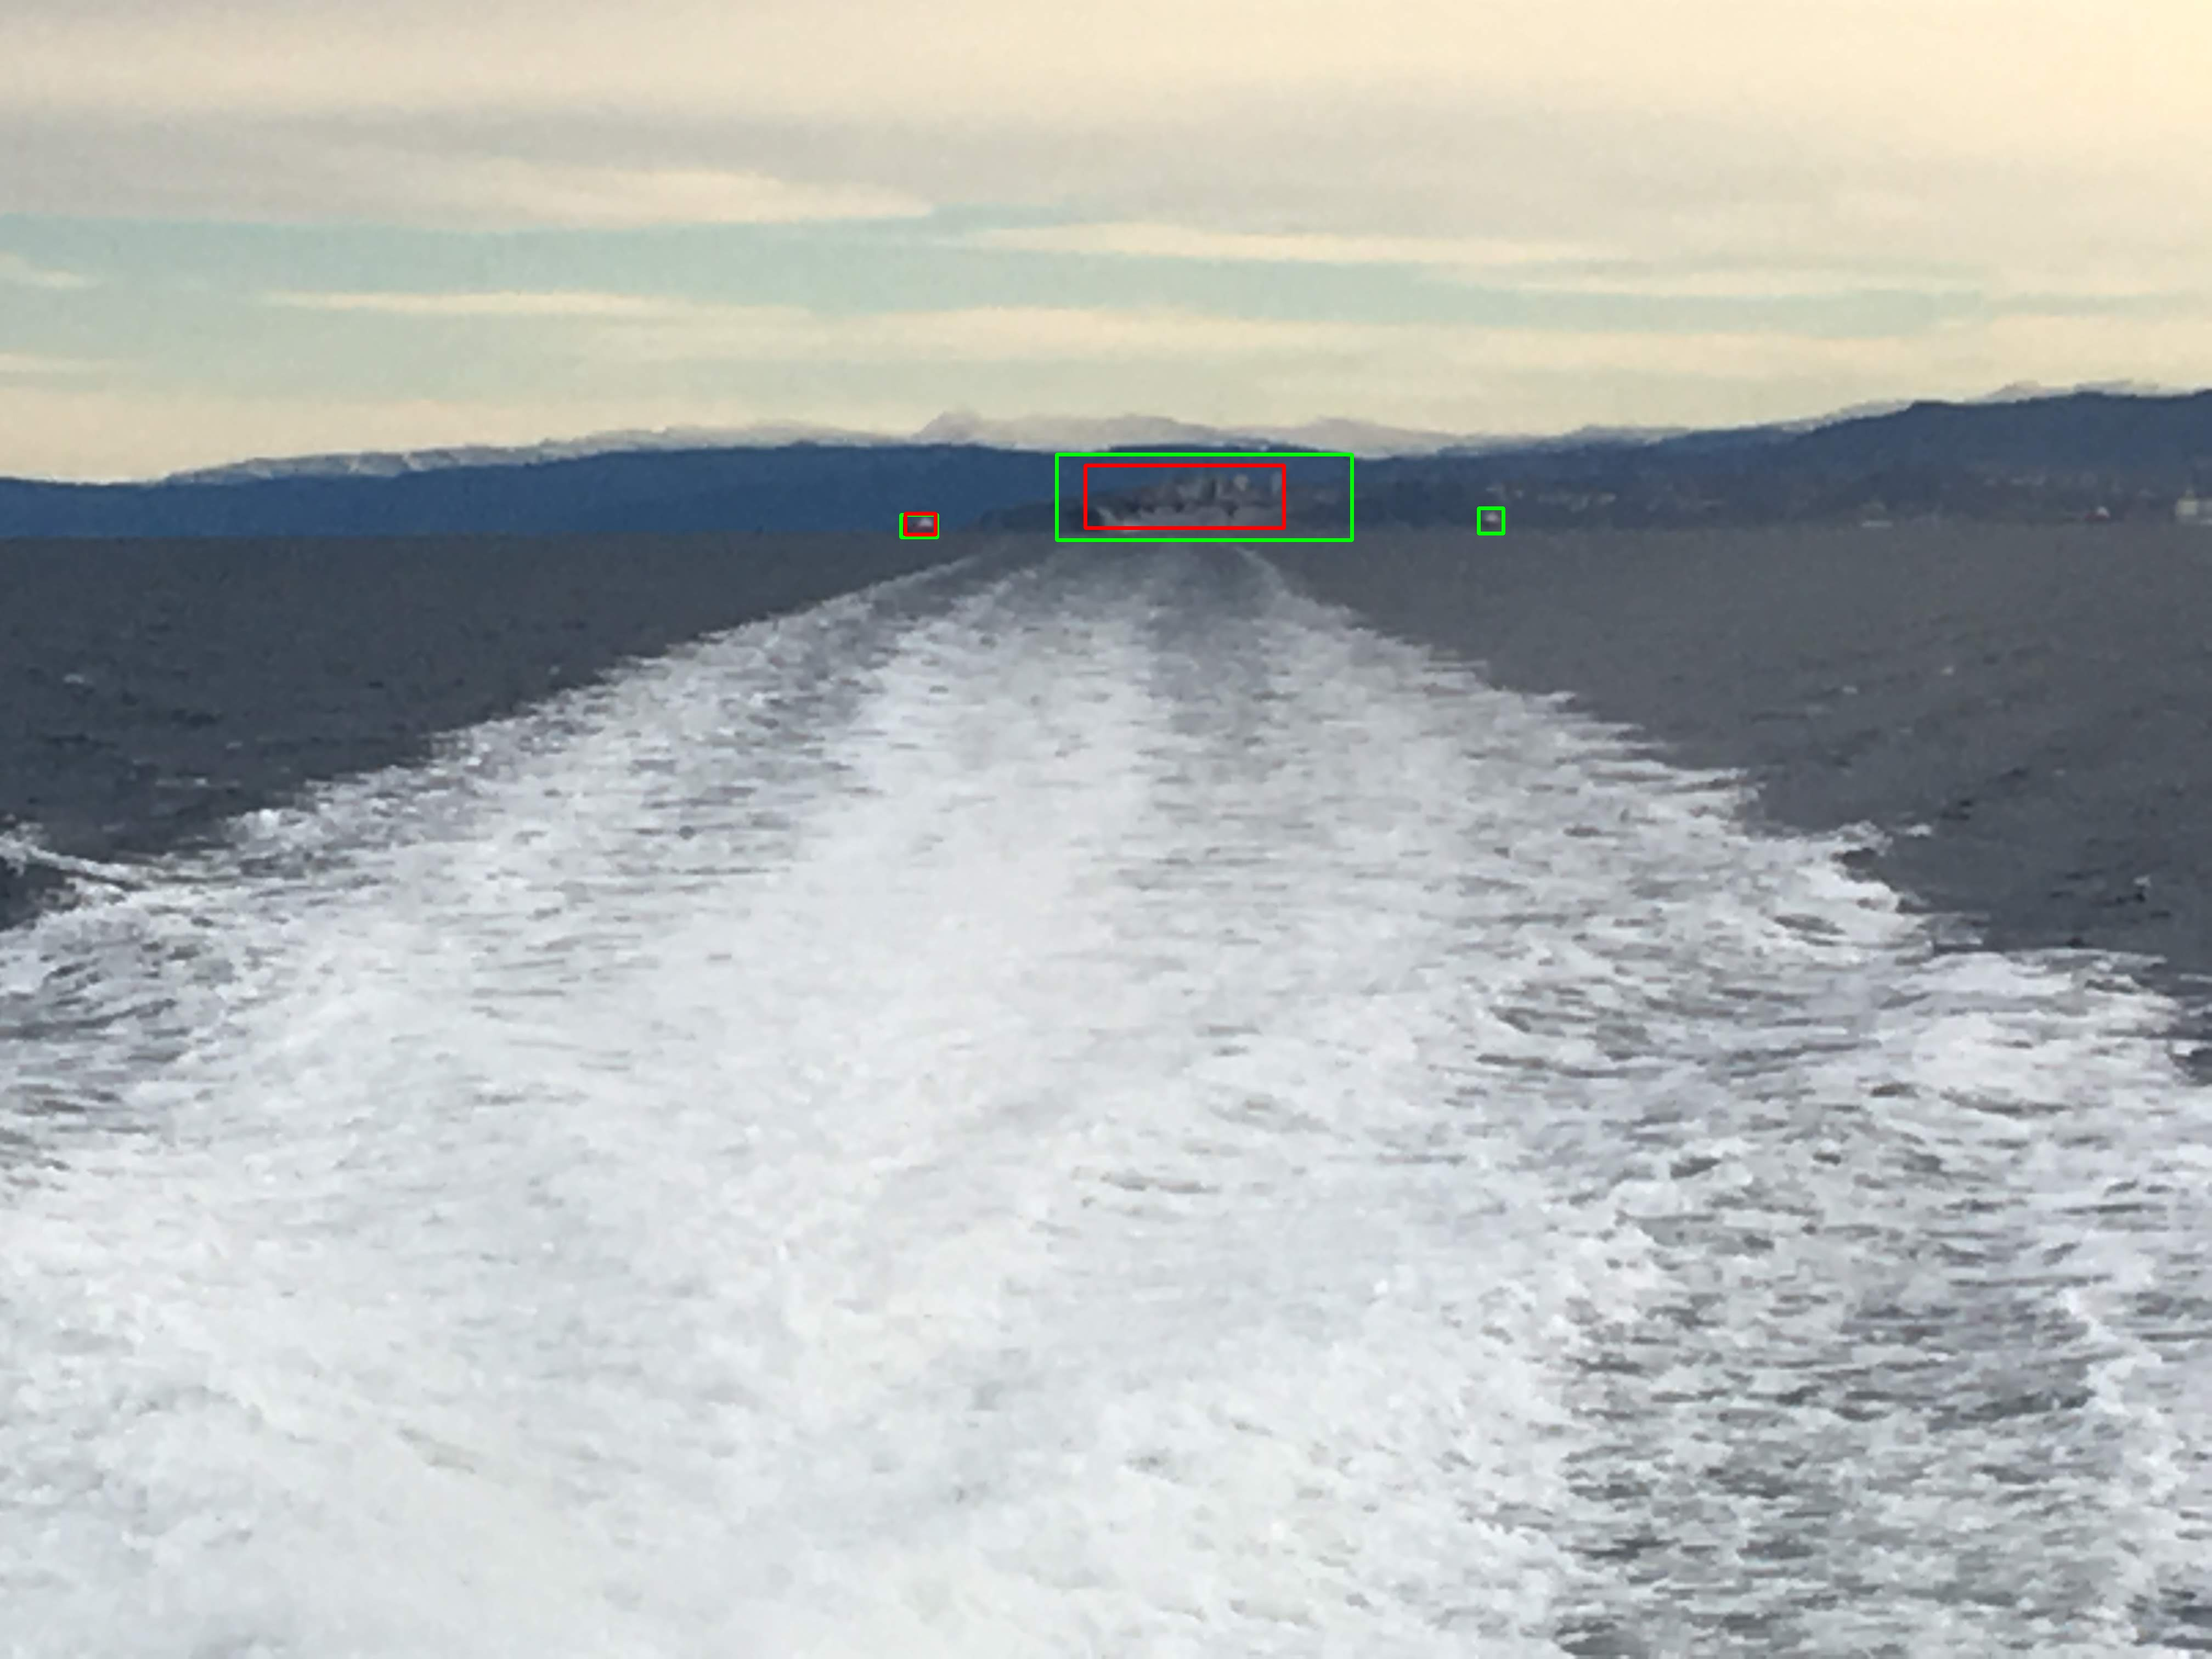
\includegraphics[width=0.8\linewidth]{results/case_buildings/yolotrf/Yolo2/IMG_2350.jpg}
  \caption{Yolo2}
  %\label{fig:ex_trf_prec_rec_yolo}
\end{subfigure}%
\begin{subfigure}{.5\textwidth}
  \centering
  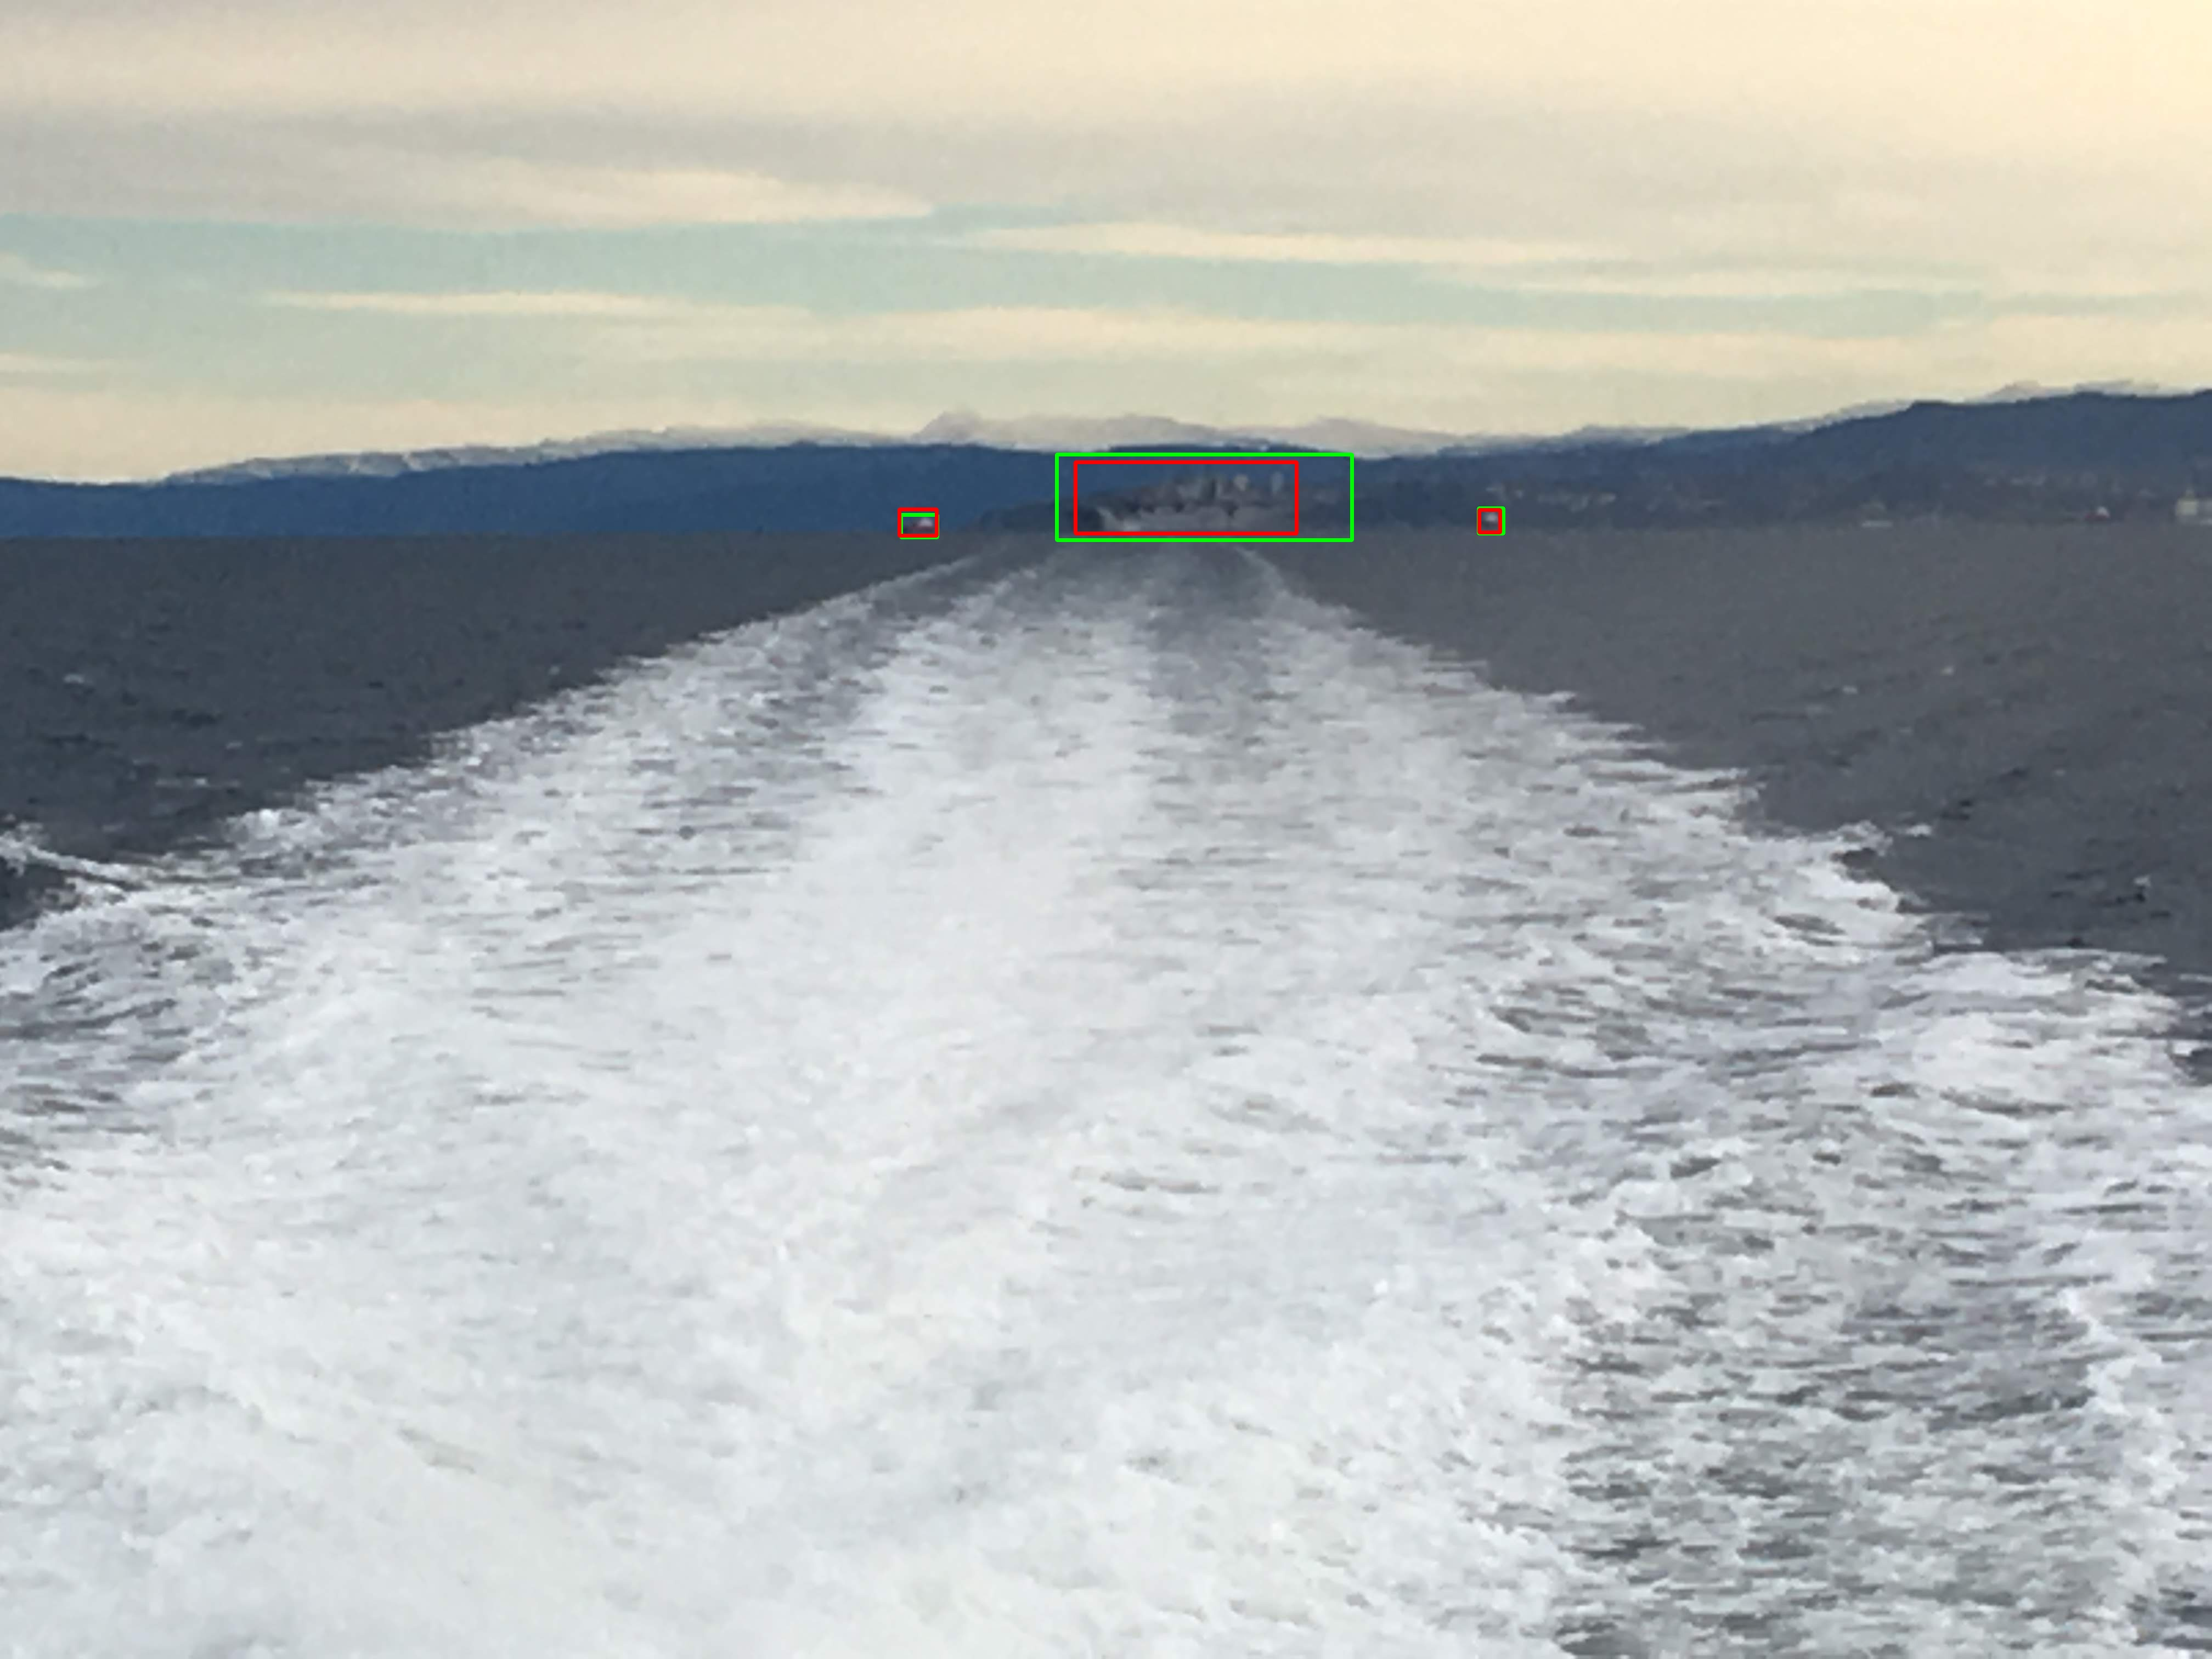
\includegraphics[width=.8\linewidth]{results/case_buildings/yolotrf/Yolo3/IMG_2350.jpg}
  \caption{Yolo3}
  %\label{fig:ex_trf_prec_rec_ssd}
\end{subfigure}
\caption{Yolo2 does not detect rightmost boat, Yolo3 does}
\label{fig:Yolo3_better_trf}
\end{figure}

\newpage
\clearpage

\section{Case Study 2: Effect of training on moored boats testing for sailing boats}
\label{sec:moored_boats}

Since Yolo3's results on \textit{trf} are nearly perfect, as shown in figure \ref{fig:moor_trf} it is necessary to investigate if the model have been fitted to this type of data in a larger extent than it should. Therefore, a case study of how training on moored boats (bbnb) affect the results on detection of sailing boats (\textit{bc}, \textit{bf}, \textit{trf}), was done. Since Yolo2's and Yolo3's results on \textit{trf} are better than Yolo1's, without more training on the same data, it could imply that the accuracy of the results are not connected to overtraining. This will be further discussed in \ref{dataset_divers}.


\begin{figure}[h!]
\begin{subfigure}{.5\textwidth}
  \centering
  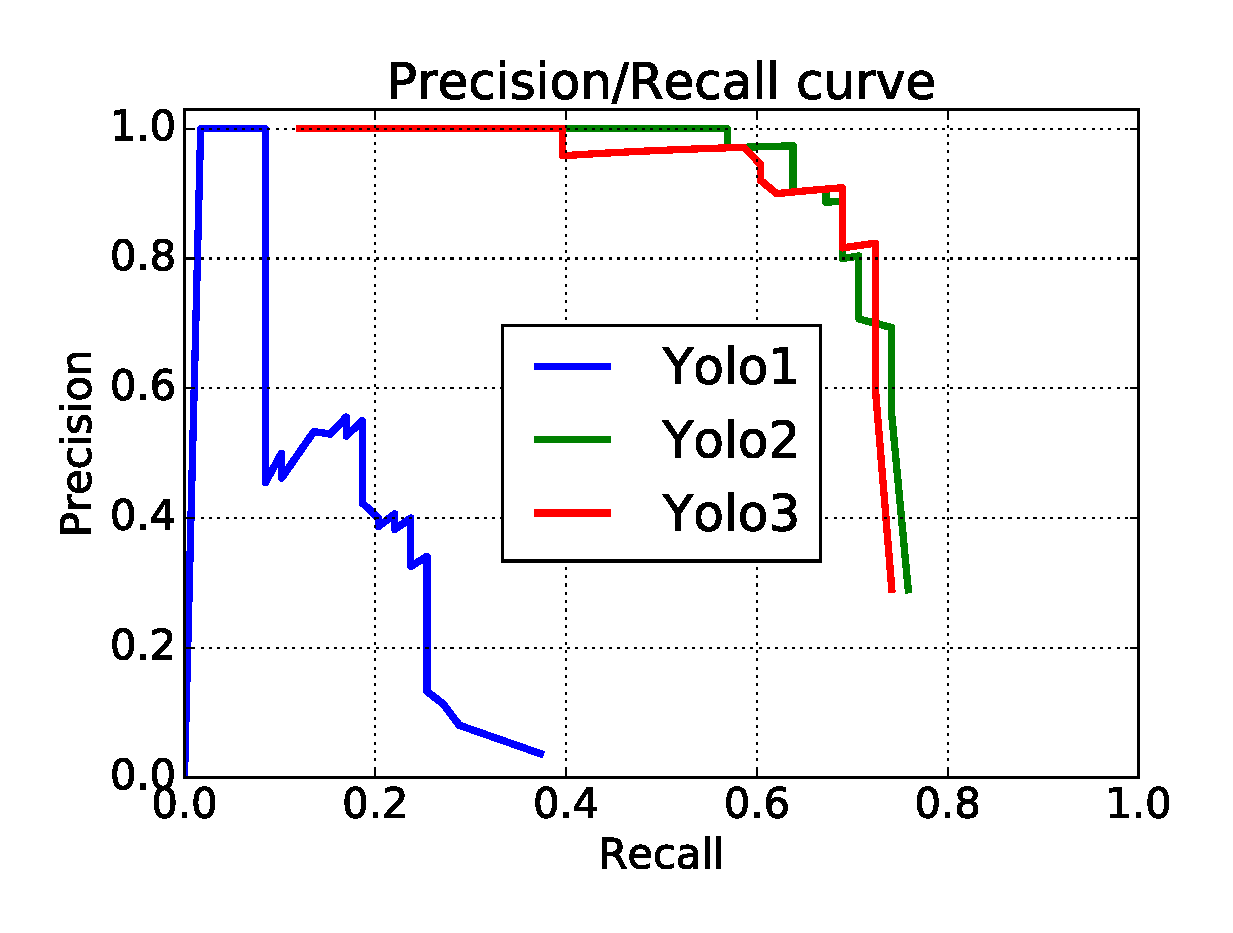
\includegraphics[width=0.8\linewidth]{results/case_tr_moor/prec_recall/bb.eps}
  \caption{Yolo1, Yolo2 and Yolo3 on bbnb}
  \label{fig:moor_bb}
\end{subfigure}%
\begin{subfigure}{.5\textwidth}
  \centering
  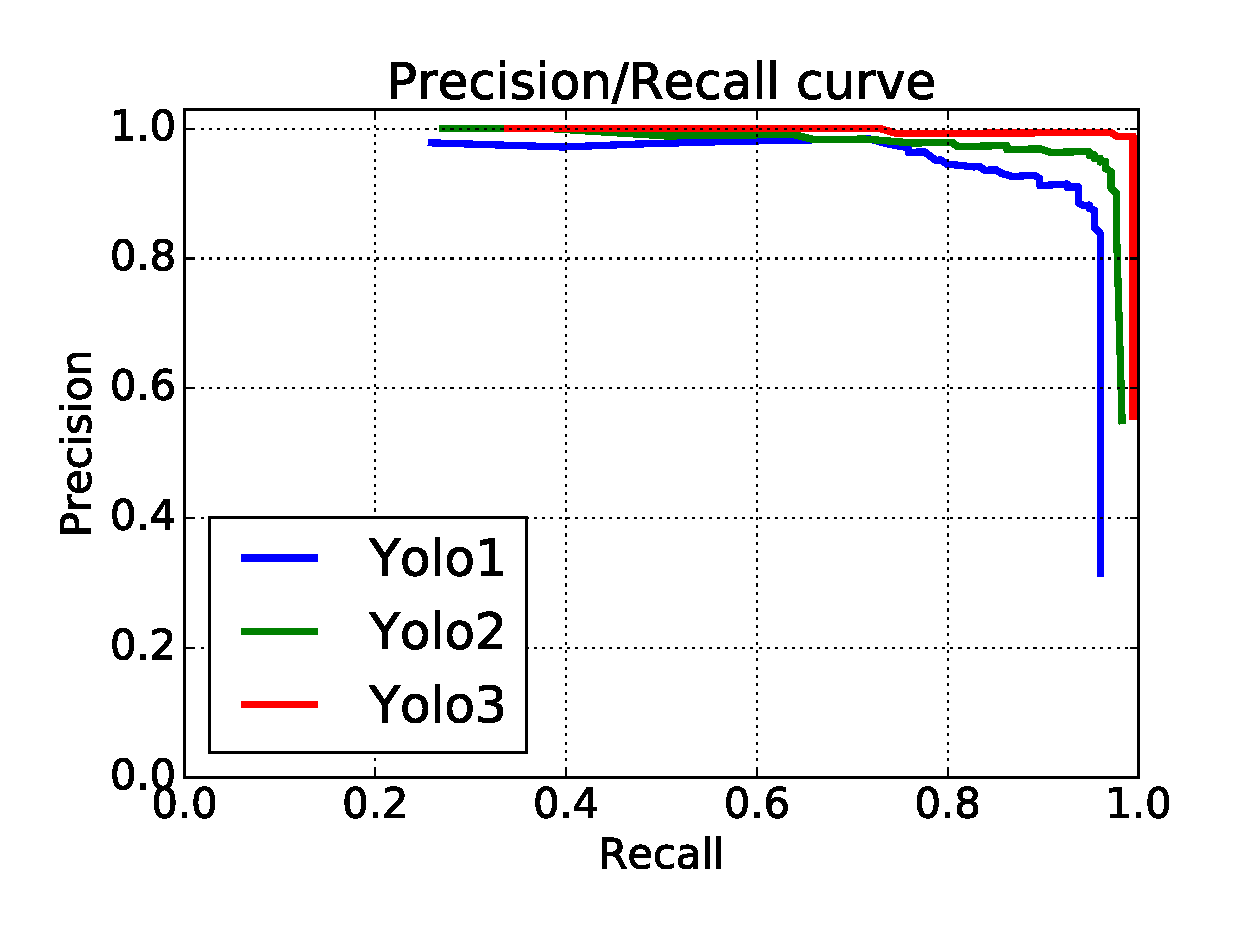
\includegraphics[width=.8\linewidth]{results/case_tr_moor/prec_recall/trf.eps}
  \caption{Yolo1, Yolo2 and Yolo3 on \textit{trf}}
  \label{fig:moor_trf}
\end{subfigure}

\begin{subfigure}{.5\textwidth}
  \centering
  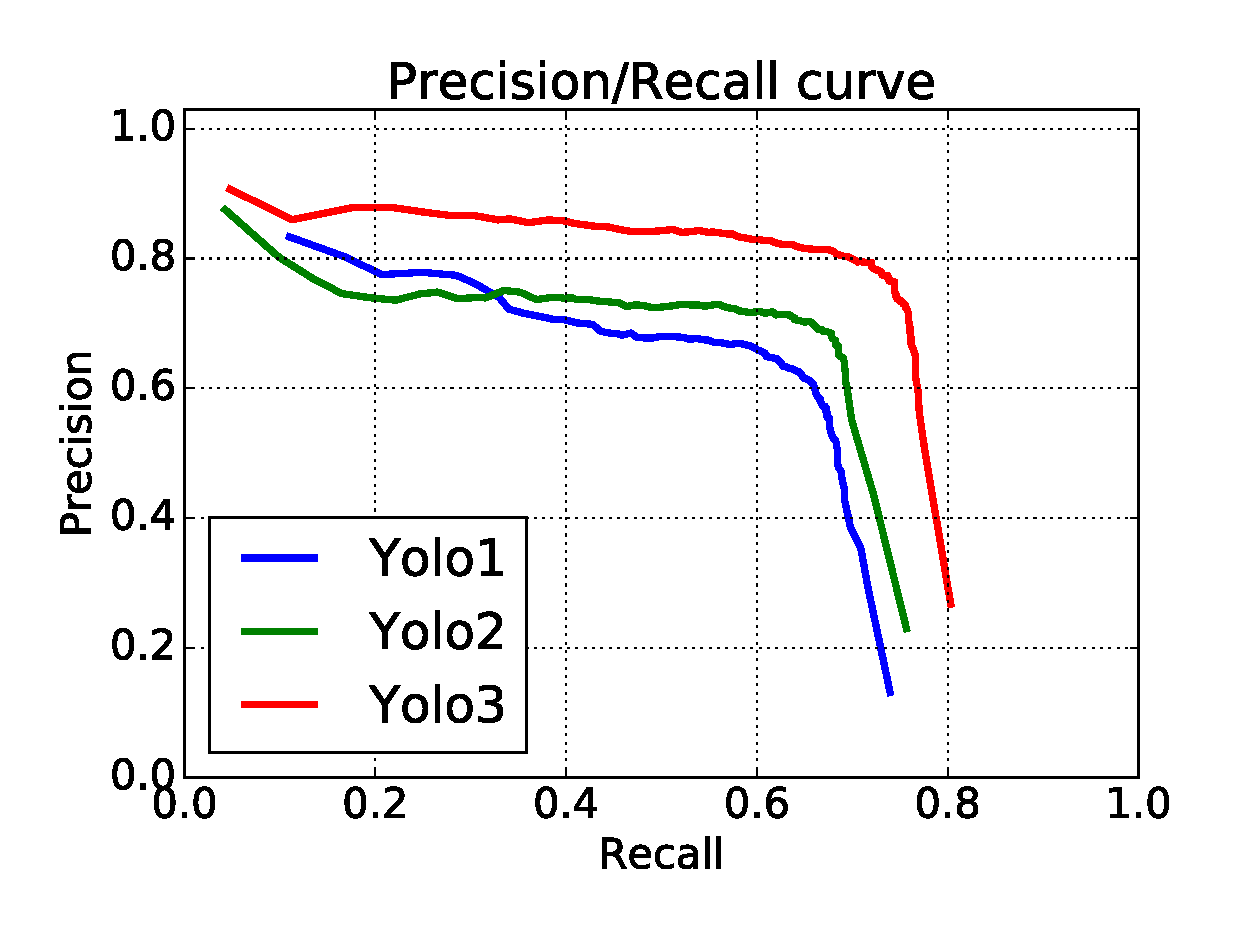
\includegraphics[width=0.8\linewidth]{results/case_tr_moor/prec_recall/bcbf.eps}
  \caption{Yolo1, Yolo2 and Yolo3 on \textit{bc}, \textit{bf}}
  %\label{fig:moor_bcbf}
\end{subfigure}%
\begin{subfigure}{.5\textwidth}
  \centering
  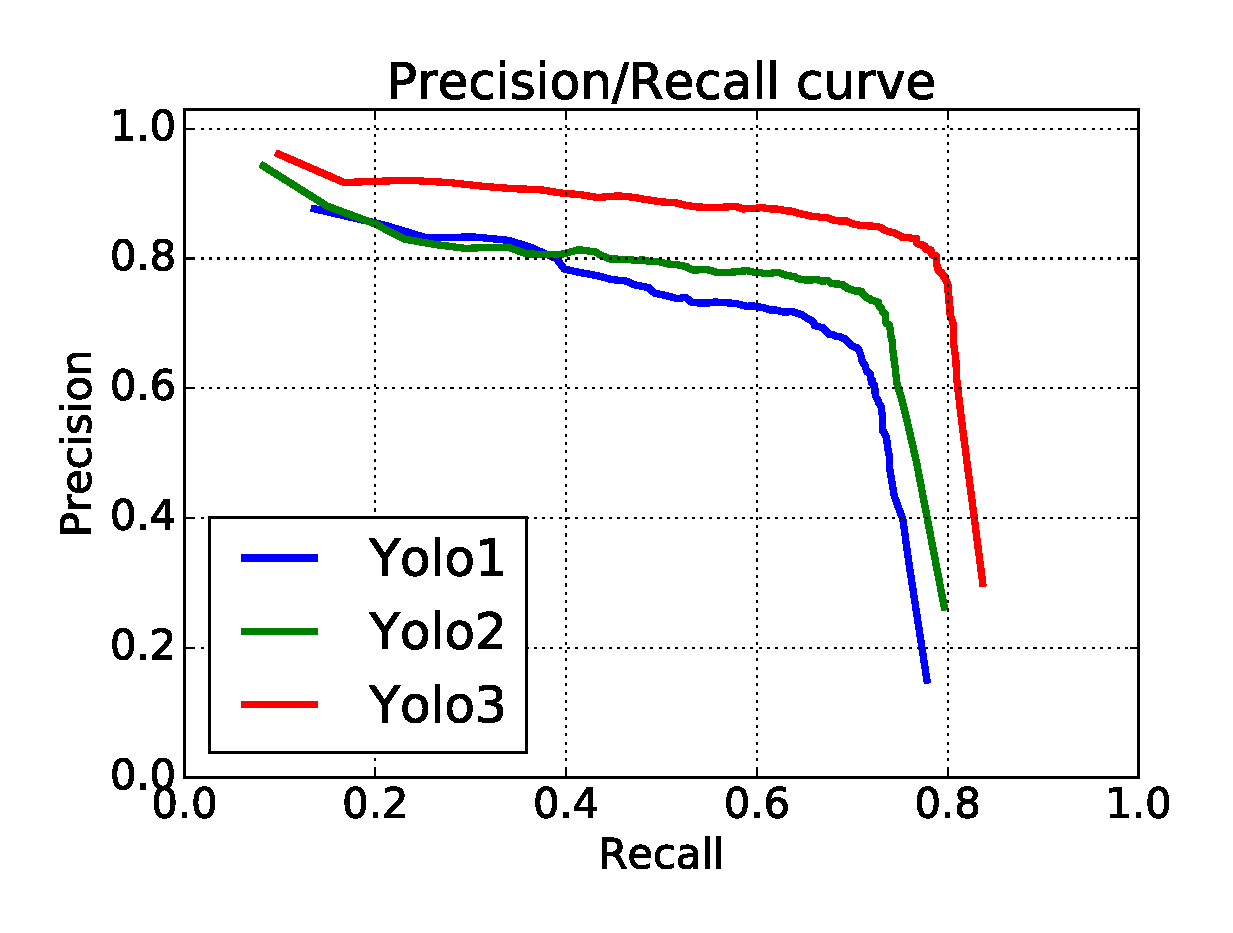
\includegraphics[width=.8\linewidth]{results/case_tr_moor/prec_recall/bcbftrf.eps}
  \caption{Yolo1, Yolo2 and Yolo3 on \textit{bc}, \textit{bf}, \textit{trf}}
  %\label{fig:moor_bcbftrf}
\end{subfigure}
\caption{Precision/recall curves for Yolo1, Yolo2, SSD1 and SSD2 on bb and on \textit{bc}, \textit{bf}, \textit{trf}}
\label{fig:prec_rec_case_moor}

\end{figure}

In figure \ref{fig:prec_rec_case_moor} the precision/recall curves for Yolo1, Yolo2 and Yolo3 are shown. Yolo2 and 3 are better than Yolo1 in all the test cases. While this is expected behavior when testing on bbnb, the results are not obvious for the other test cases. 

\vspace{3mm}

Two clear differences between Yolo1 and Yolo2 were found while analyzing the results. The first one being that Yolo1 tends to overestimate the size of large ships, as shown in figure \ref{fig:yolo12_big}. More examples of this behavior can be seen in Appendix C, chapter \ref{sec:yolo1_big_box}

\begin{figure}[h!]
\begin{subfigure}{.5\textwidth}
  \centering
  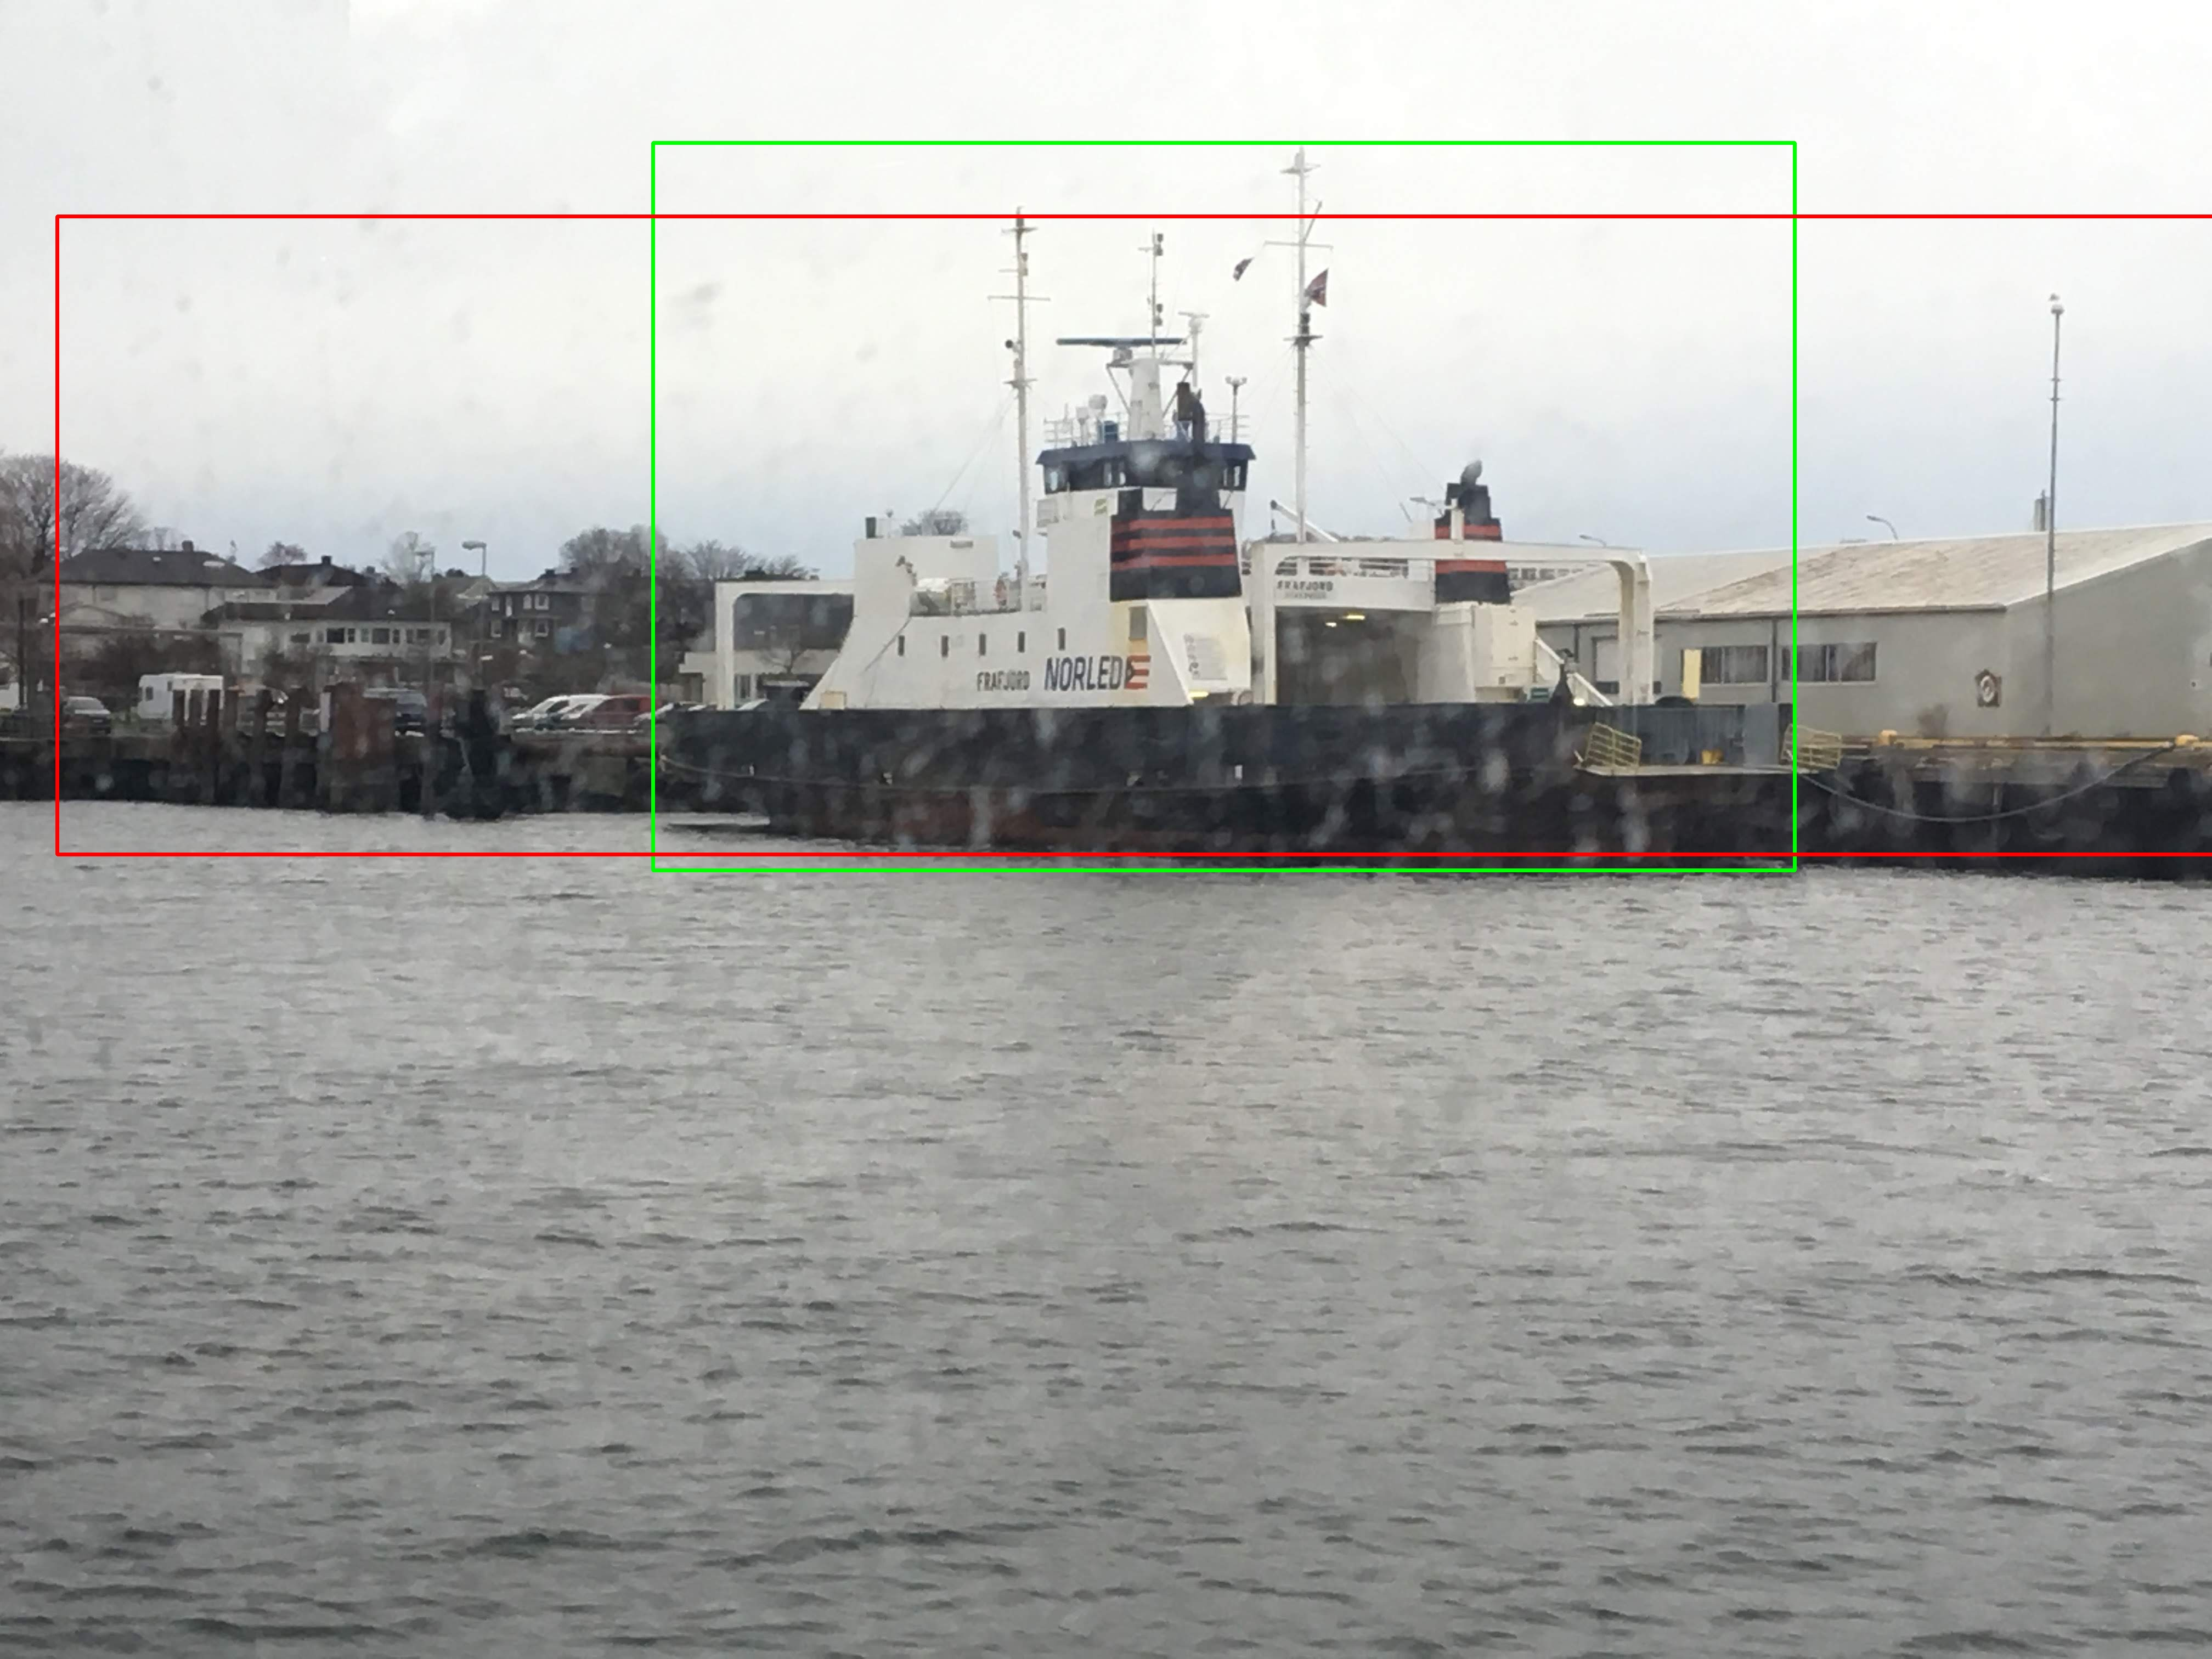
\includegraphics[width=0.8\linewidth]{results/case_tr_moor/yolo12/yolo1/big/IMG_2566.jpg}
  \caption{Yolo1}
  \label{fig:yolo1_big}
\end{subfigure}%
\begin{subfigure}{.5\textwidth}
  \centering
  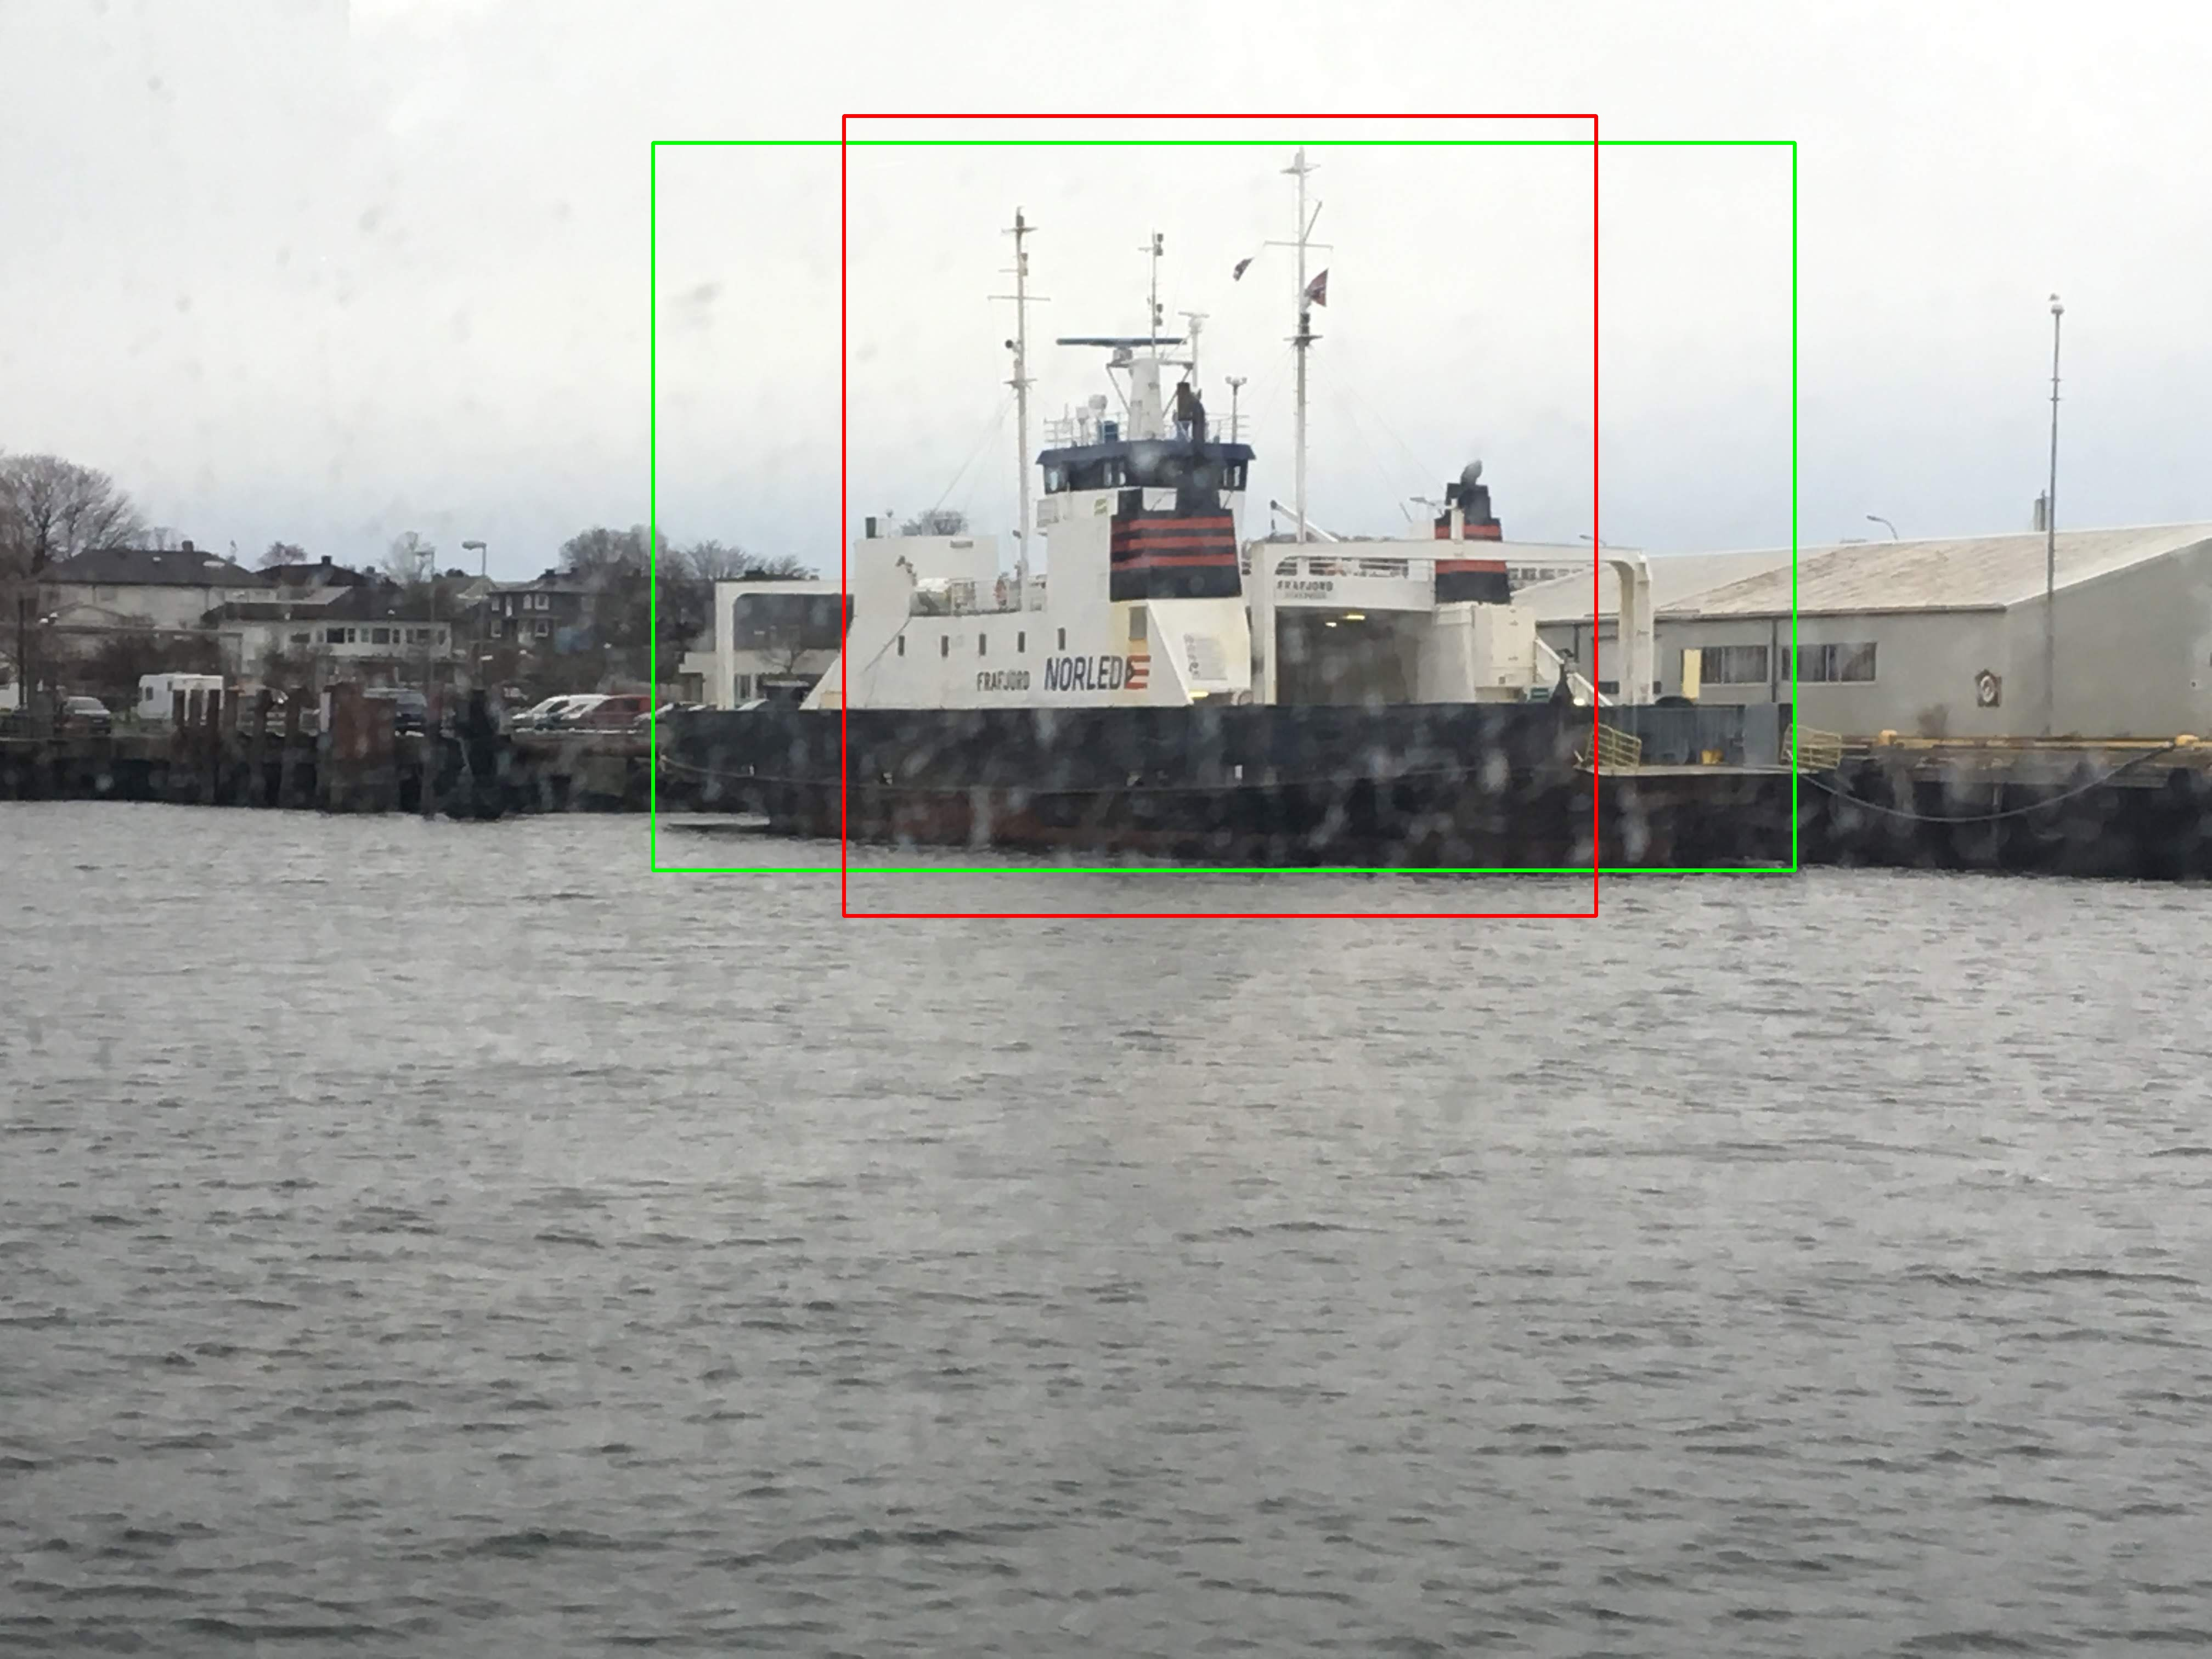
\includegraphics[width=.8\linewidth]{results/case_tr_moor/yolo12/yolo2/big/IMG_2566.jpg}
  \caption{Yolo2}
  \label{fig:yolo2_big}
\end{subfigure}
\caption{Example of Yolo1 over estimating size of ship}
\label{fig:yolo12_big}
\end{figure}

\newpage

Yolo1 also has a penchant to detect the same boat twice, where Yolo2 does not, as shown in figure \ref{fig:yolo12_multibox}. More examples of this behavior are shown in Appendix C, chapter \ref{sec:yolo1_multidetect}.

\begin{figure}[h!]
\begin{subfigure}{.5\textwidth}
  \centering
  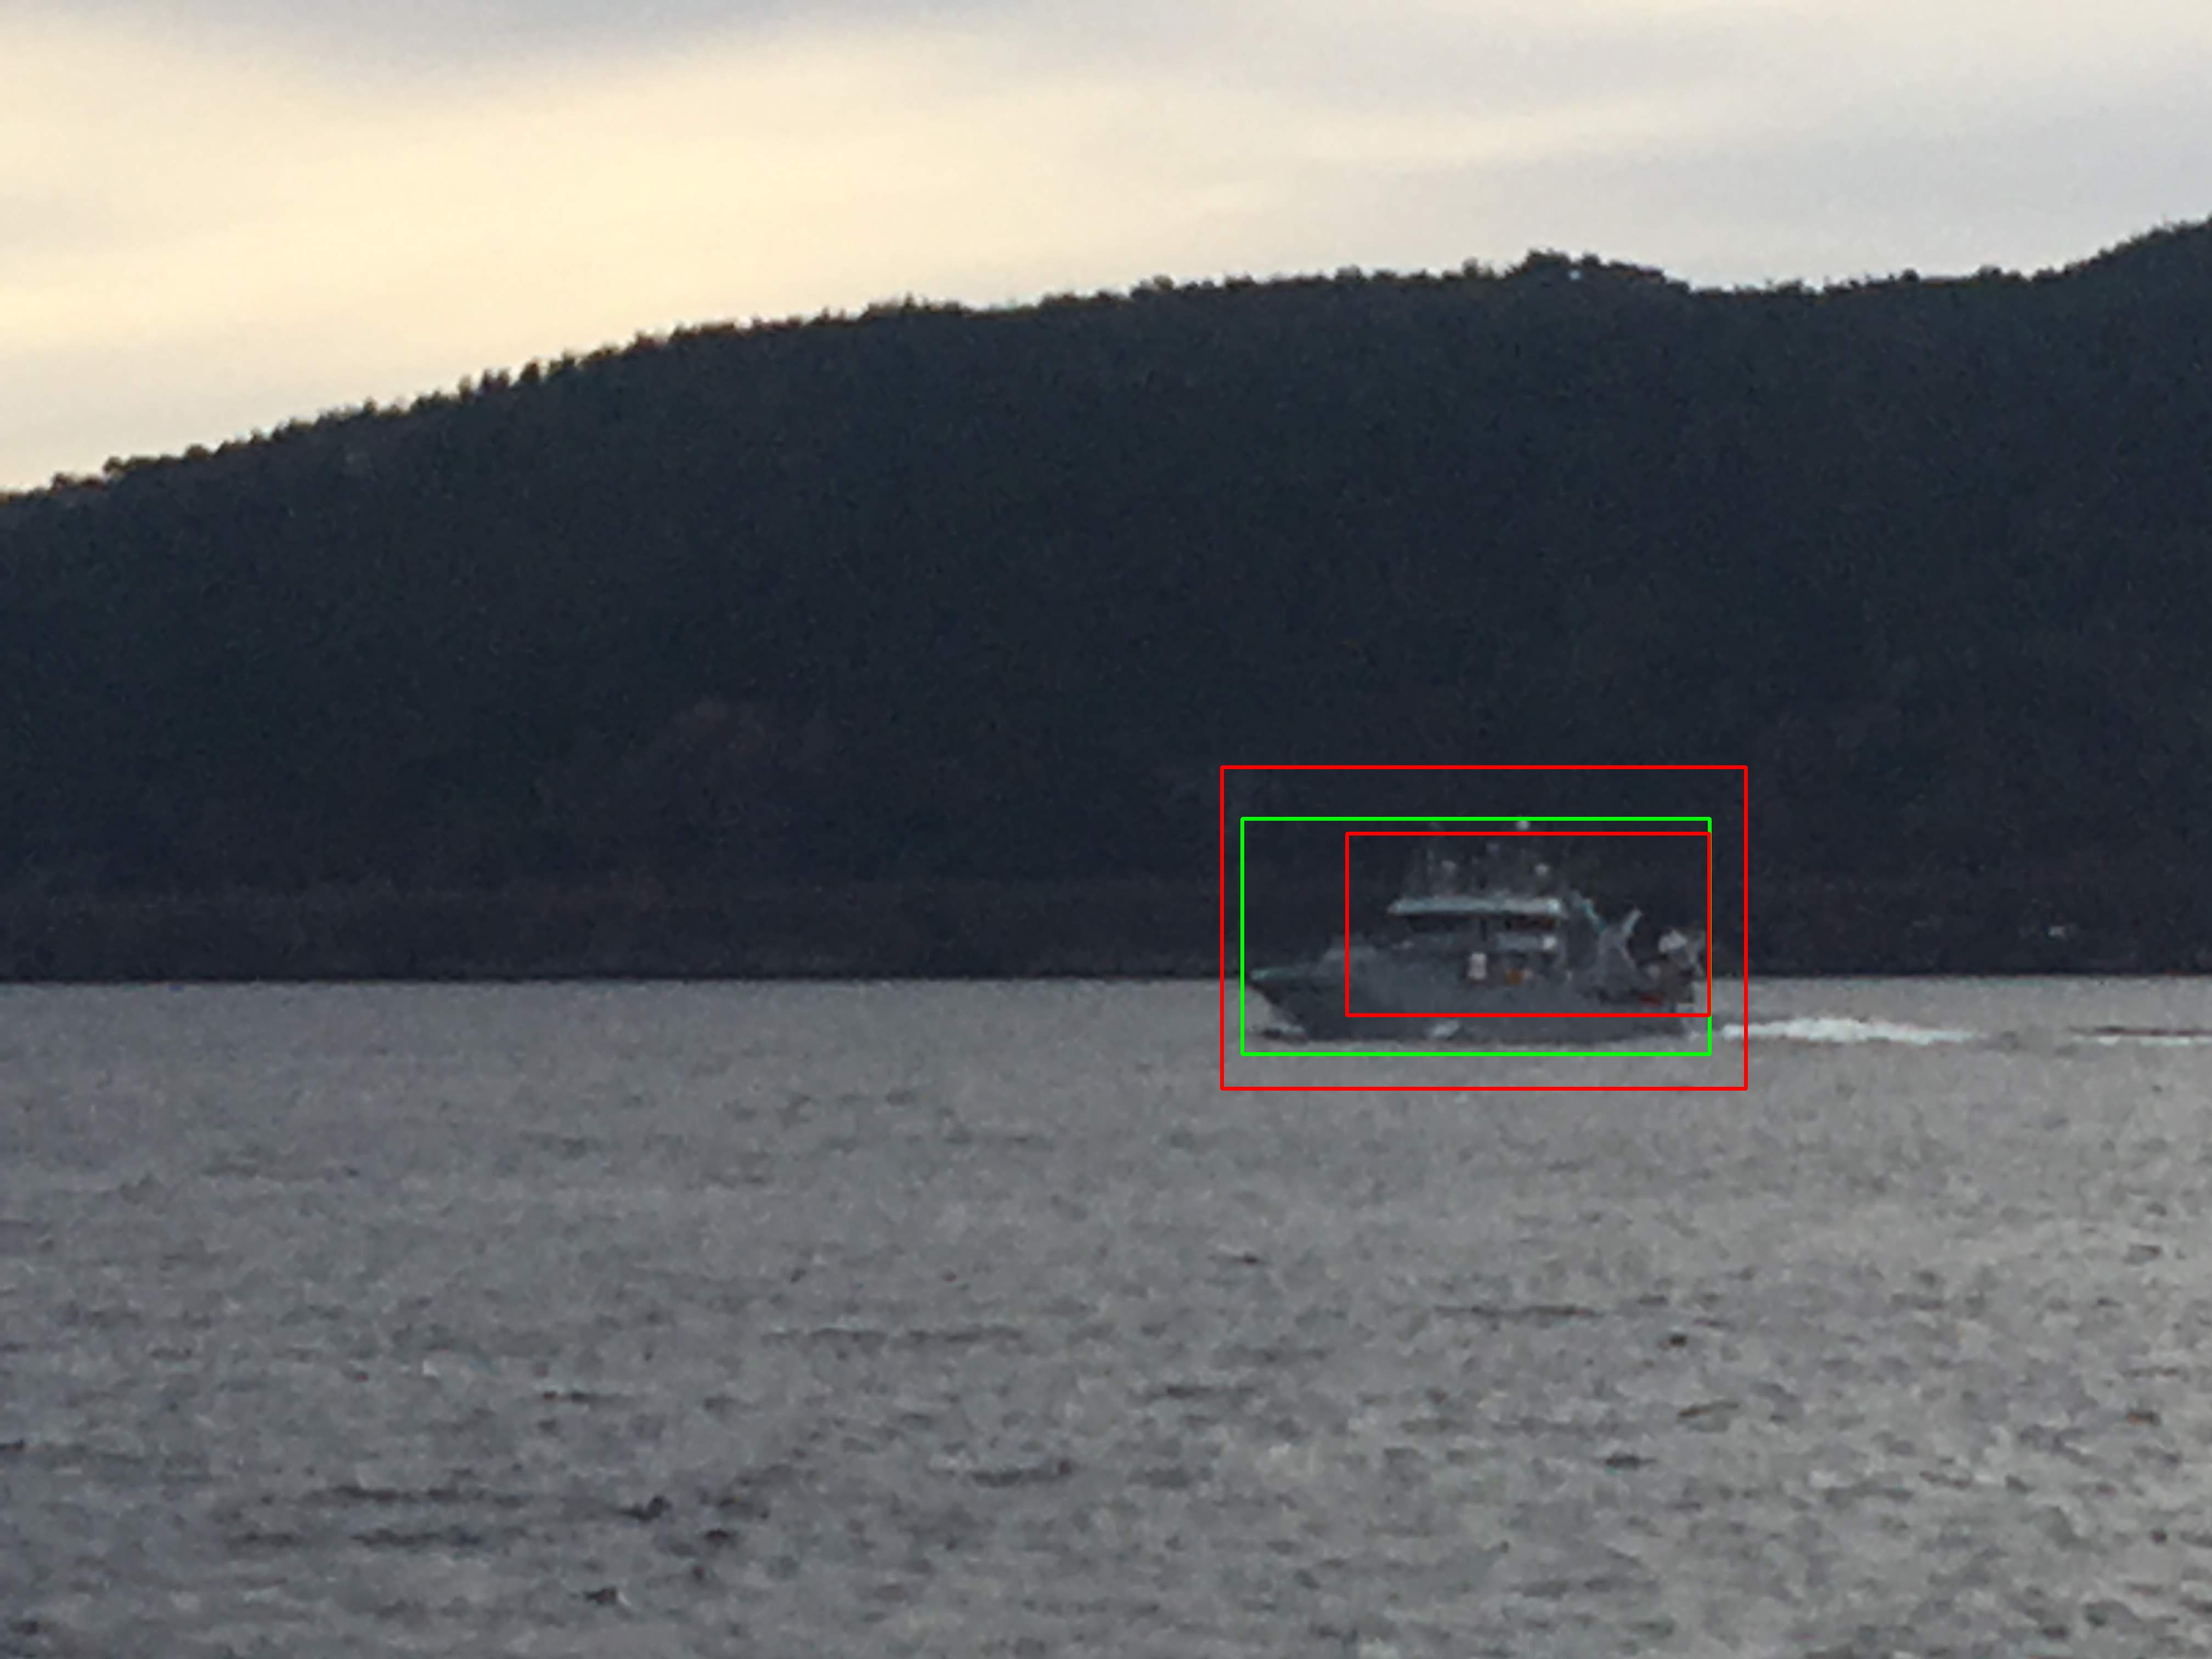
\includegraphics[width=0.8\linewidth]{results/case_tr_moor/yolo12/yolo1/2better/IMG_2269.jpg}
  \caption{Yolo1}
  \label{fig:yolo1_multibox}
\end{subfigure}%
\begin{subfigure}{.5\textwidth}
  \centering
  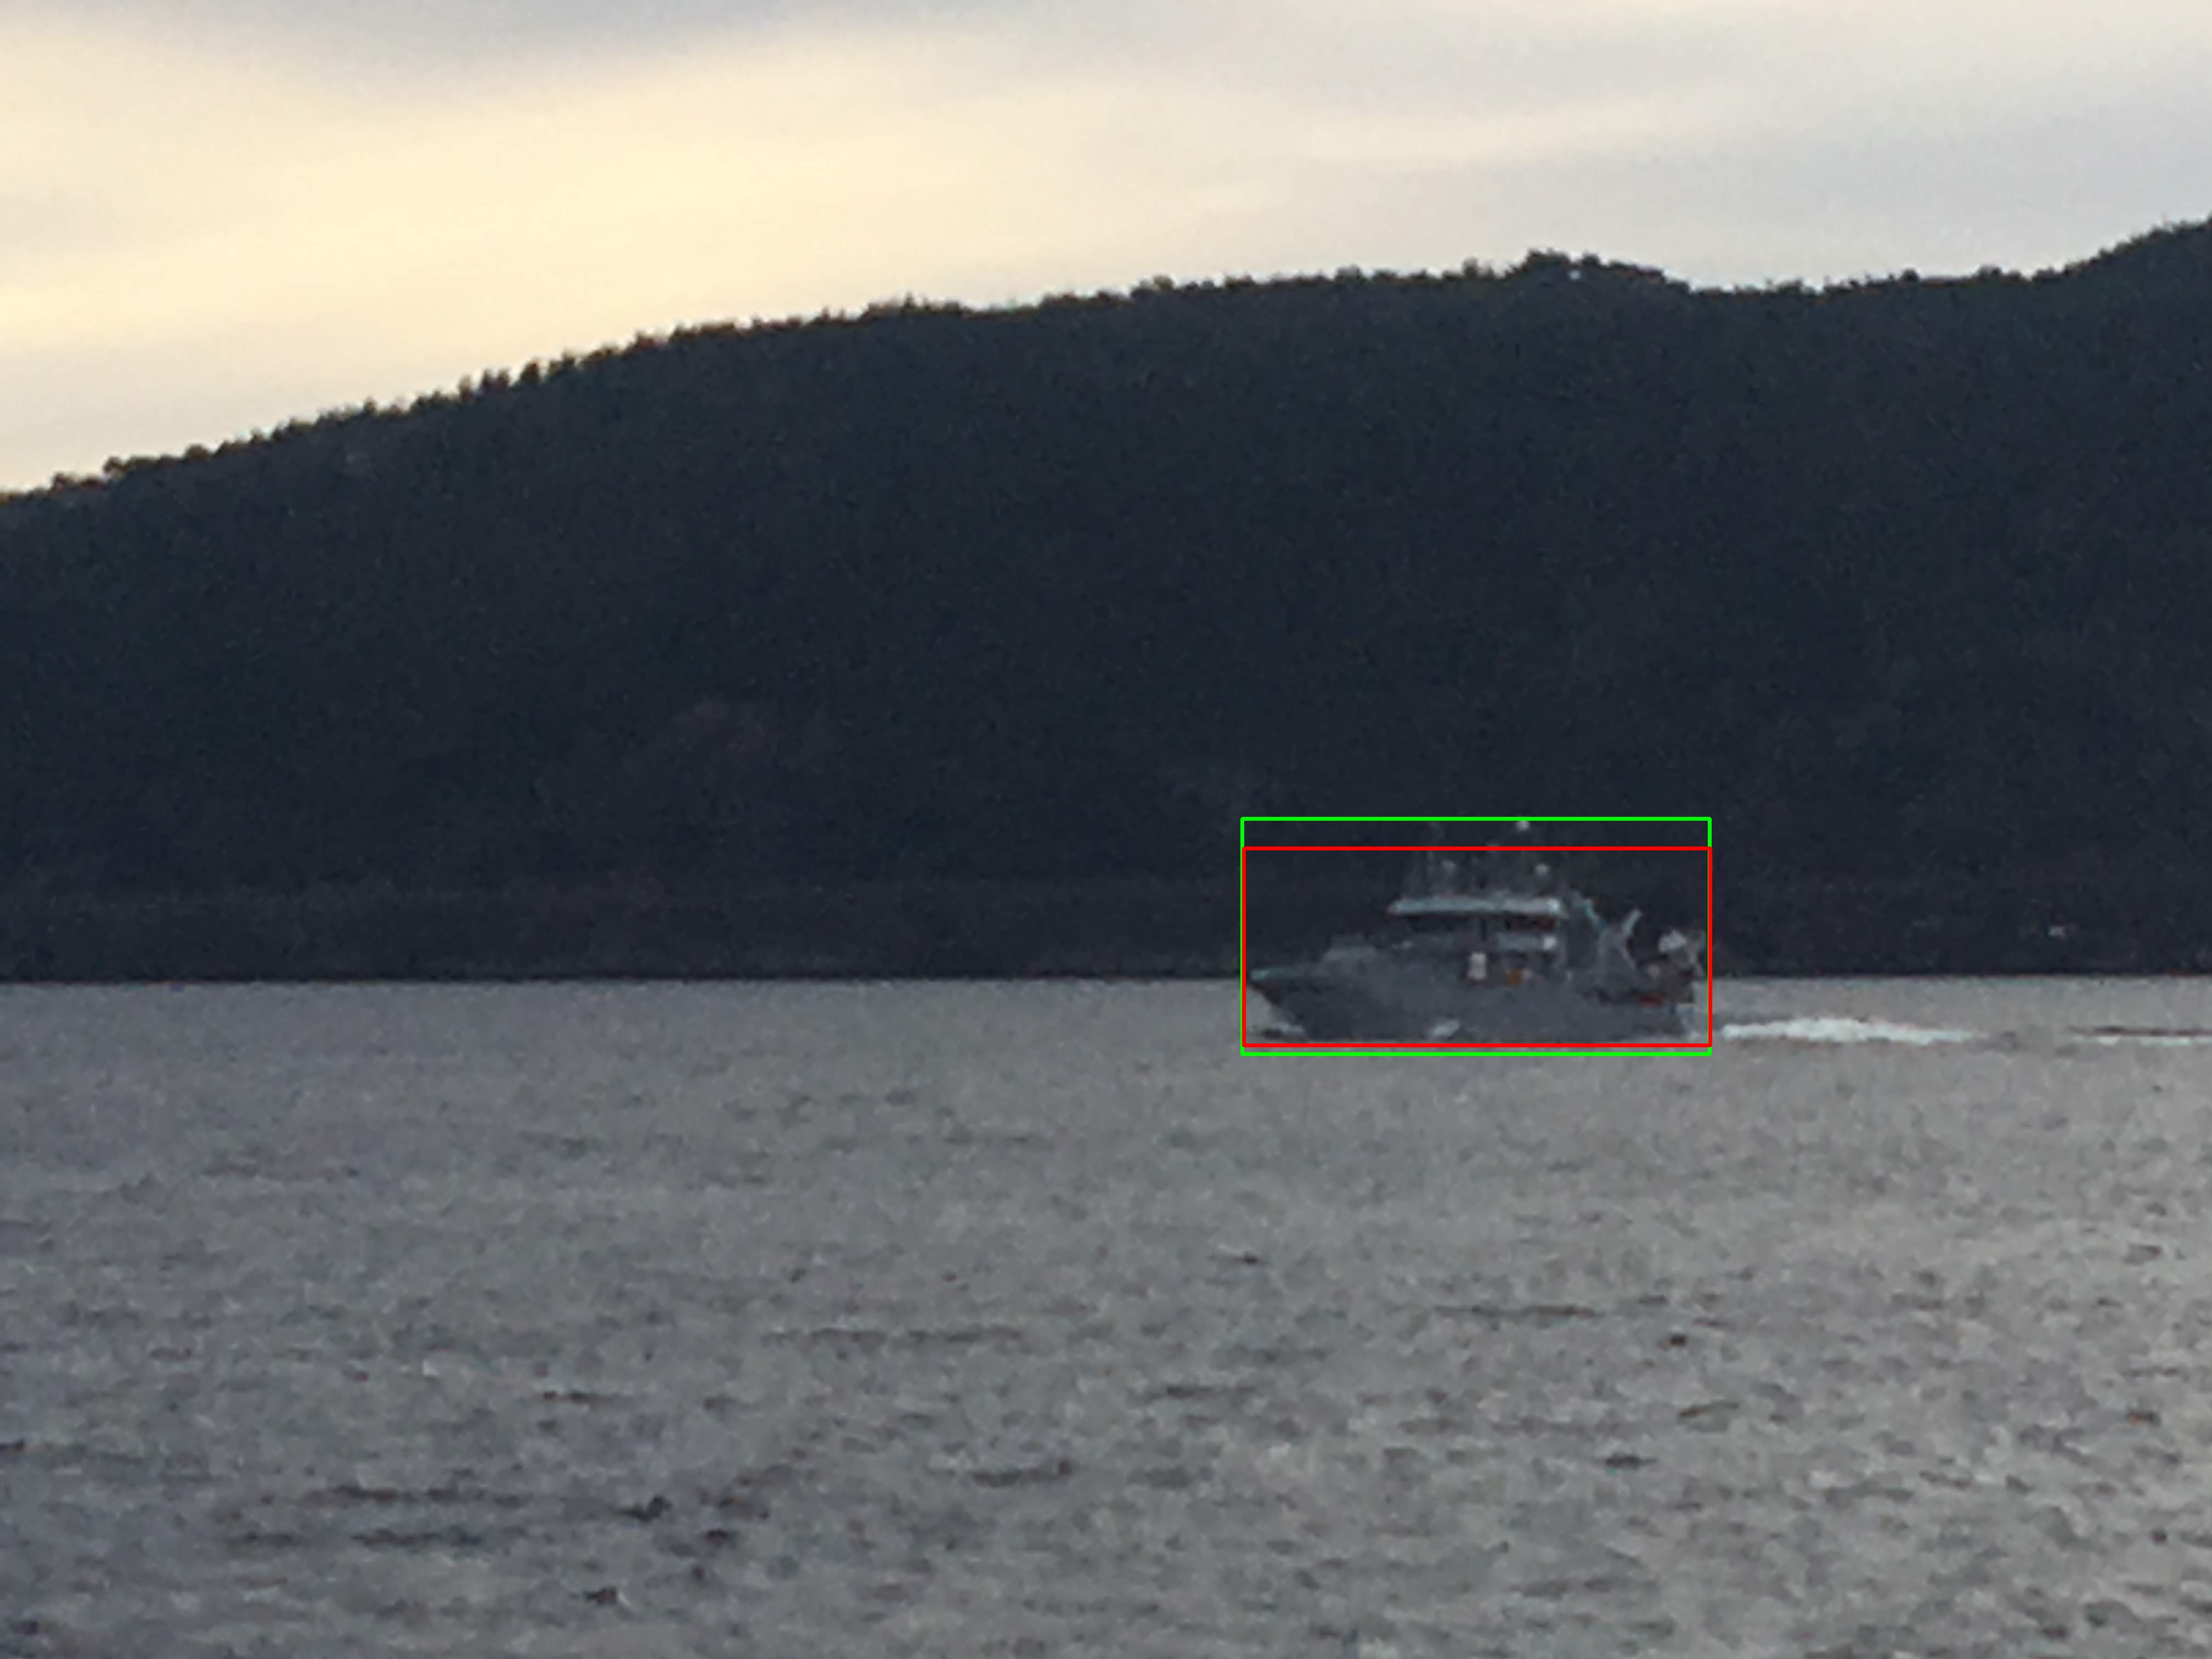
\includegraphics[width=.8\linewidth]{results/case_tr_moor/yolo12/yolo2/2better/IMG_2269.jpg}
  \caption{Yolo2}
  \label{fig:yolo2_multibox}
\end{subfigure}
\caption{Example of Yolo1 detecting same boat twice}
\label{fig:yolo12_multibox}
\end{figure}

\newpage

\section{Case Study 3: Video streaks}
In \citep{Bohn2018} the issue of detections in data over time is addressed, and is to referred to as \textit{streaks}. The goal is to make a detector that robustly detects boats in a video. This does not necessarily mean that the boat needs to be detected in every frame of a video since this can be solved e.g., by using a Markov chain as in \citep{Markov}. Still, the boat needs to be detected by some frequency, for the tracking algorithm to be able to track it. To implement a tracking algorithm is not a part of this project. However, an experiment on how well the detection algorithms work on video has been done. 

\vspace{3mm}

Three videos of boats in the Trondheim fjord have been captured, each approximately 20 seconds long. Yolo1 was tested on each of them. The three videos are merged and available at \url{https://www.youtube.com/watch?v=kcirhao_PQc}. Frames from each of the videos are shown in figure \ref{fig:videos}.

\begin{figure}[h!]
\centering
\begin{subfigure}[b]{0.78\textwidth}
   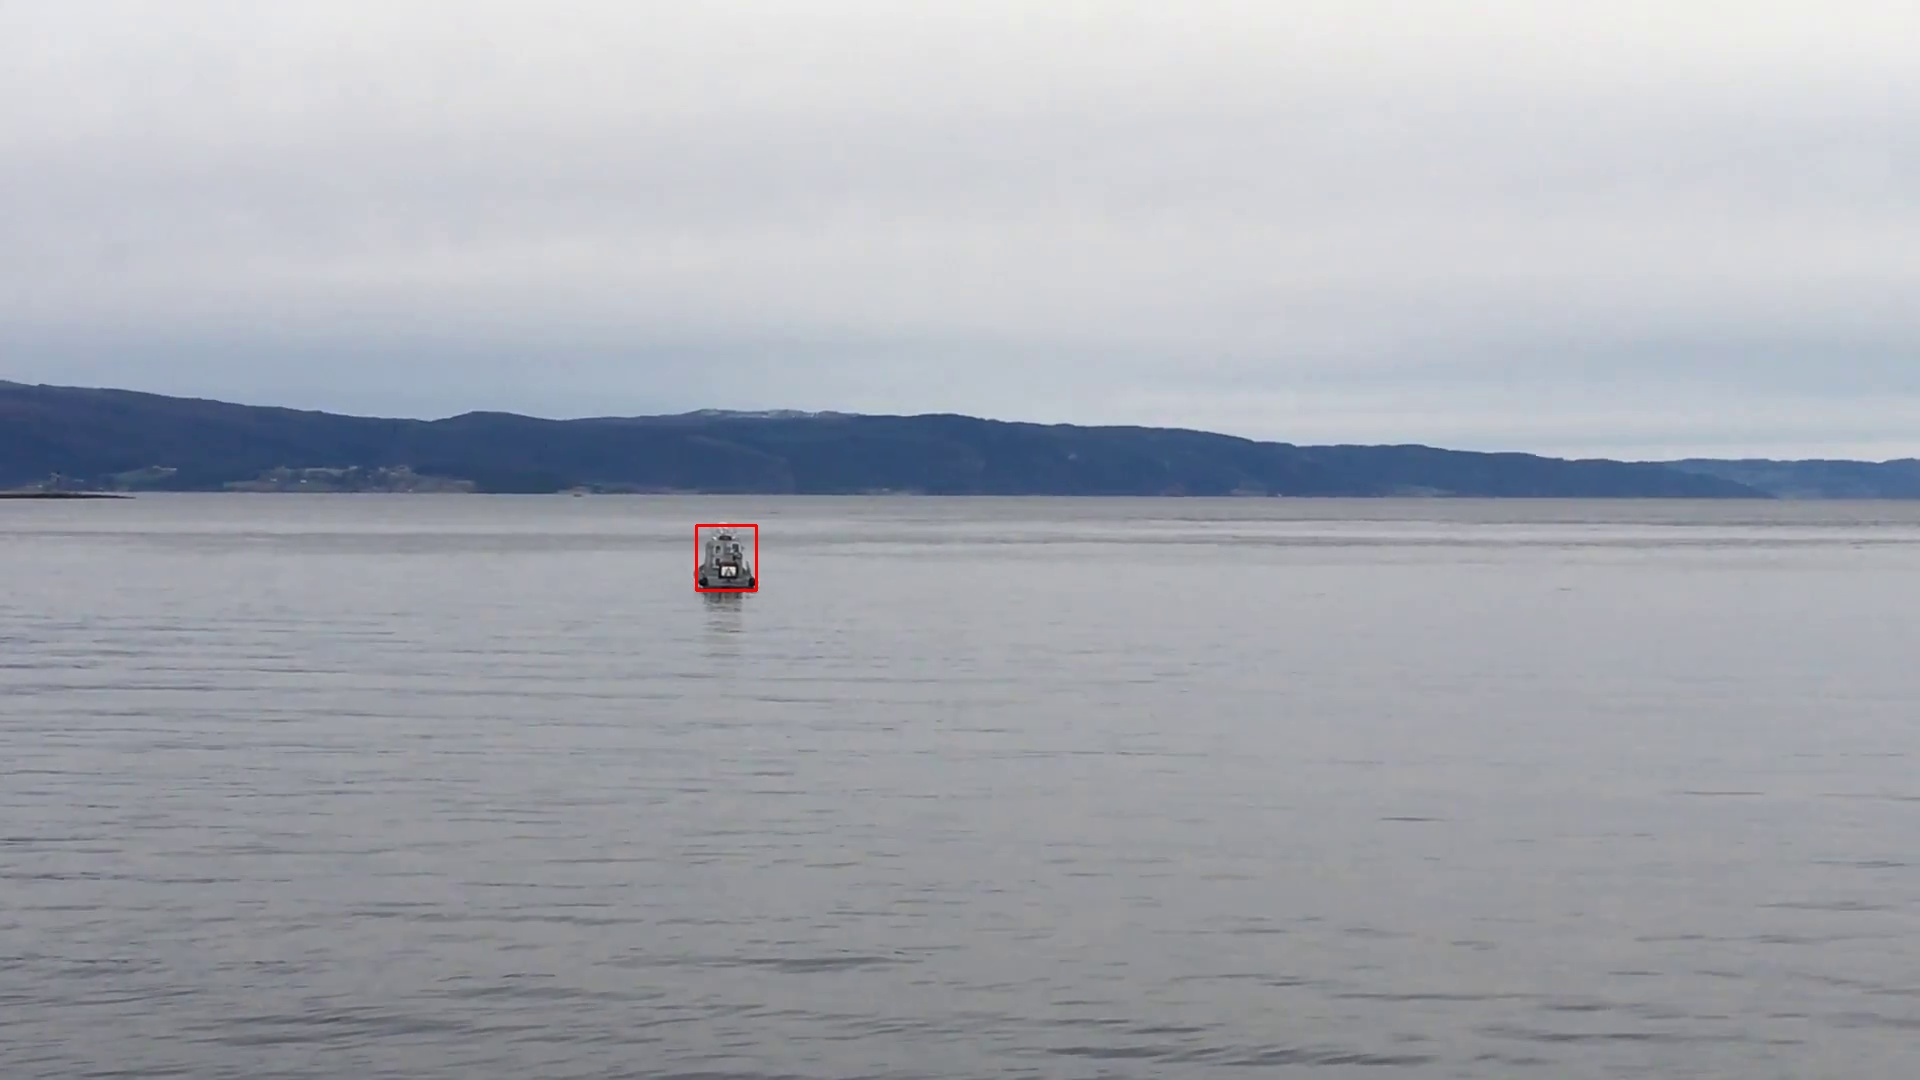
\includegraphics[width=1\linewidth]{results/video/video1/frame35.jpg}
   \caption{Video1}
   \label{fig:video1} 
\end{subfigure}

\begin{subfigure}[b]{0.78\textwidth}
   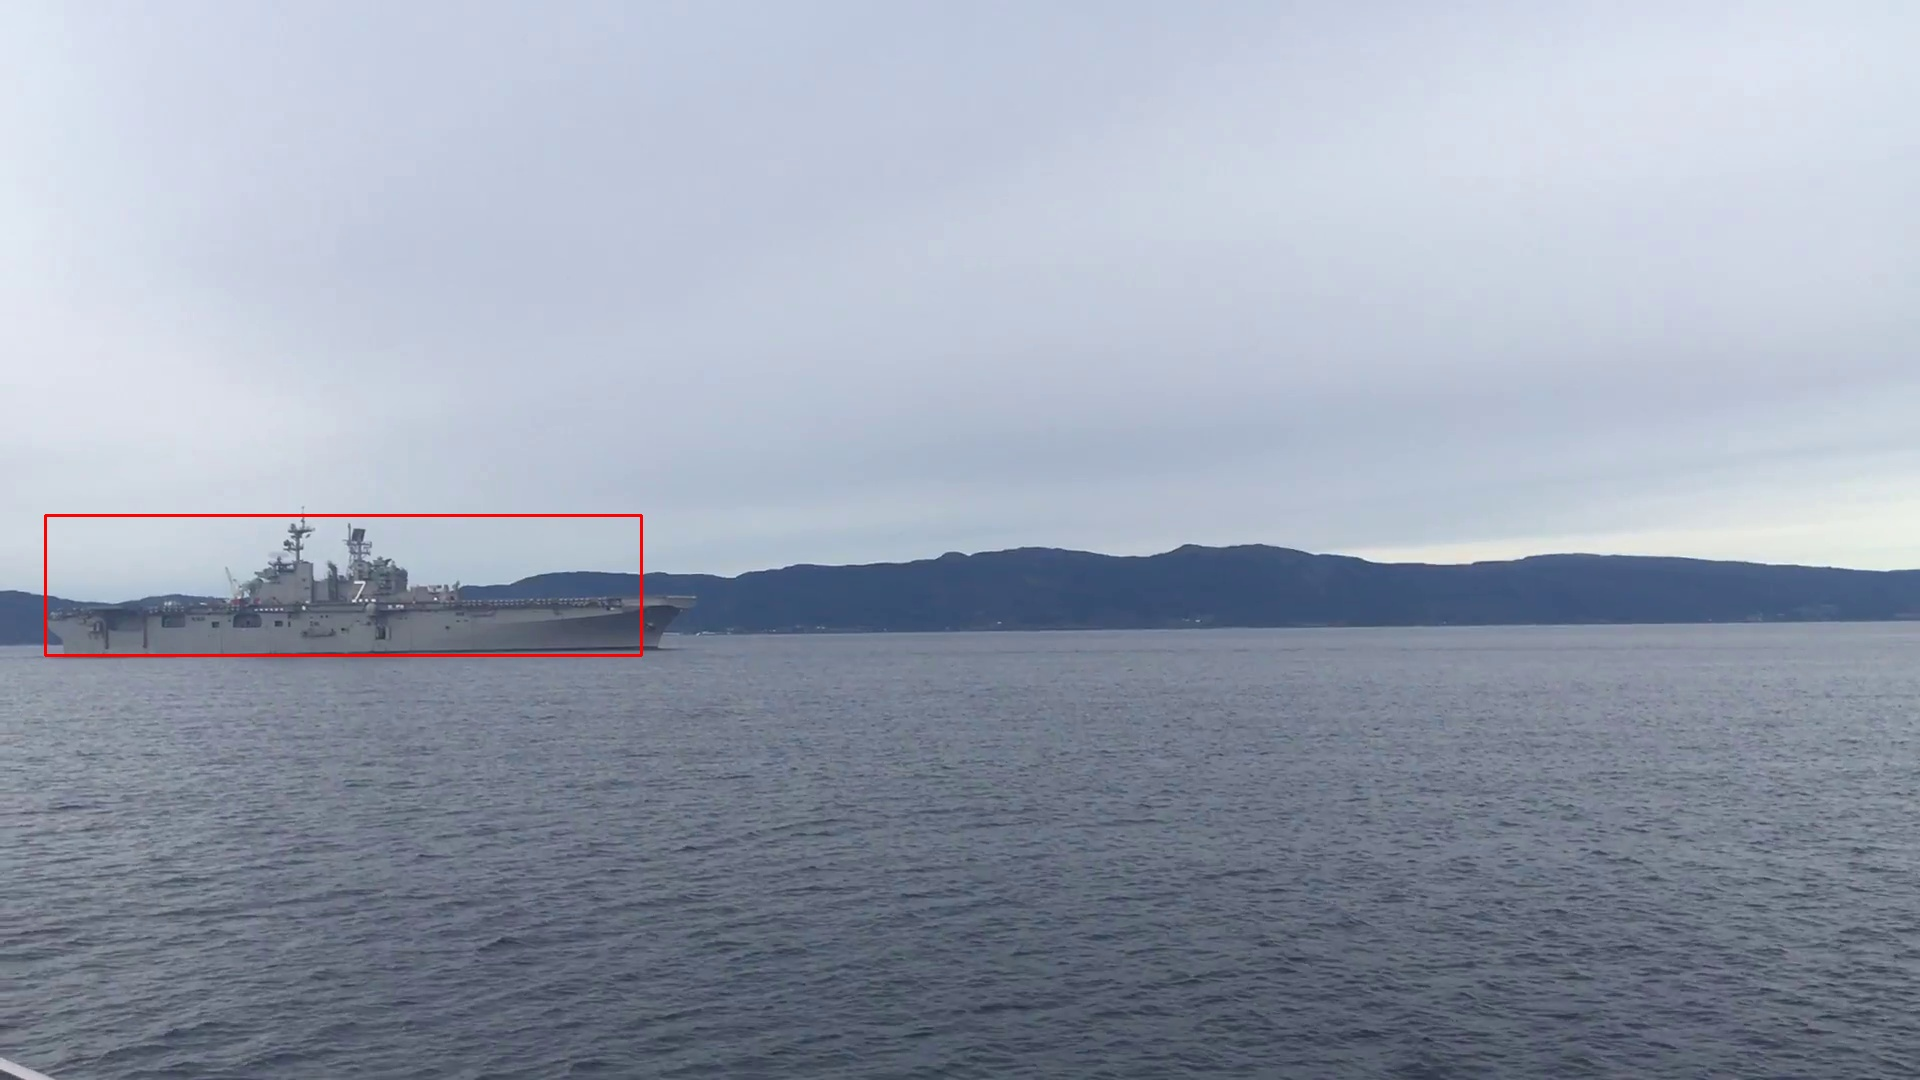
\includegraphics[width=1\linewidth]{results/video/video2/frame3.jpg}
   \caption{Video2}
   \label{fig:video2}
\end{subfigure}

\begin{subfigure}[b]{0.78\textwidth}
   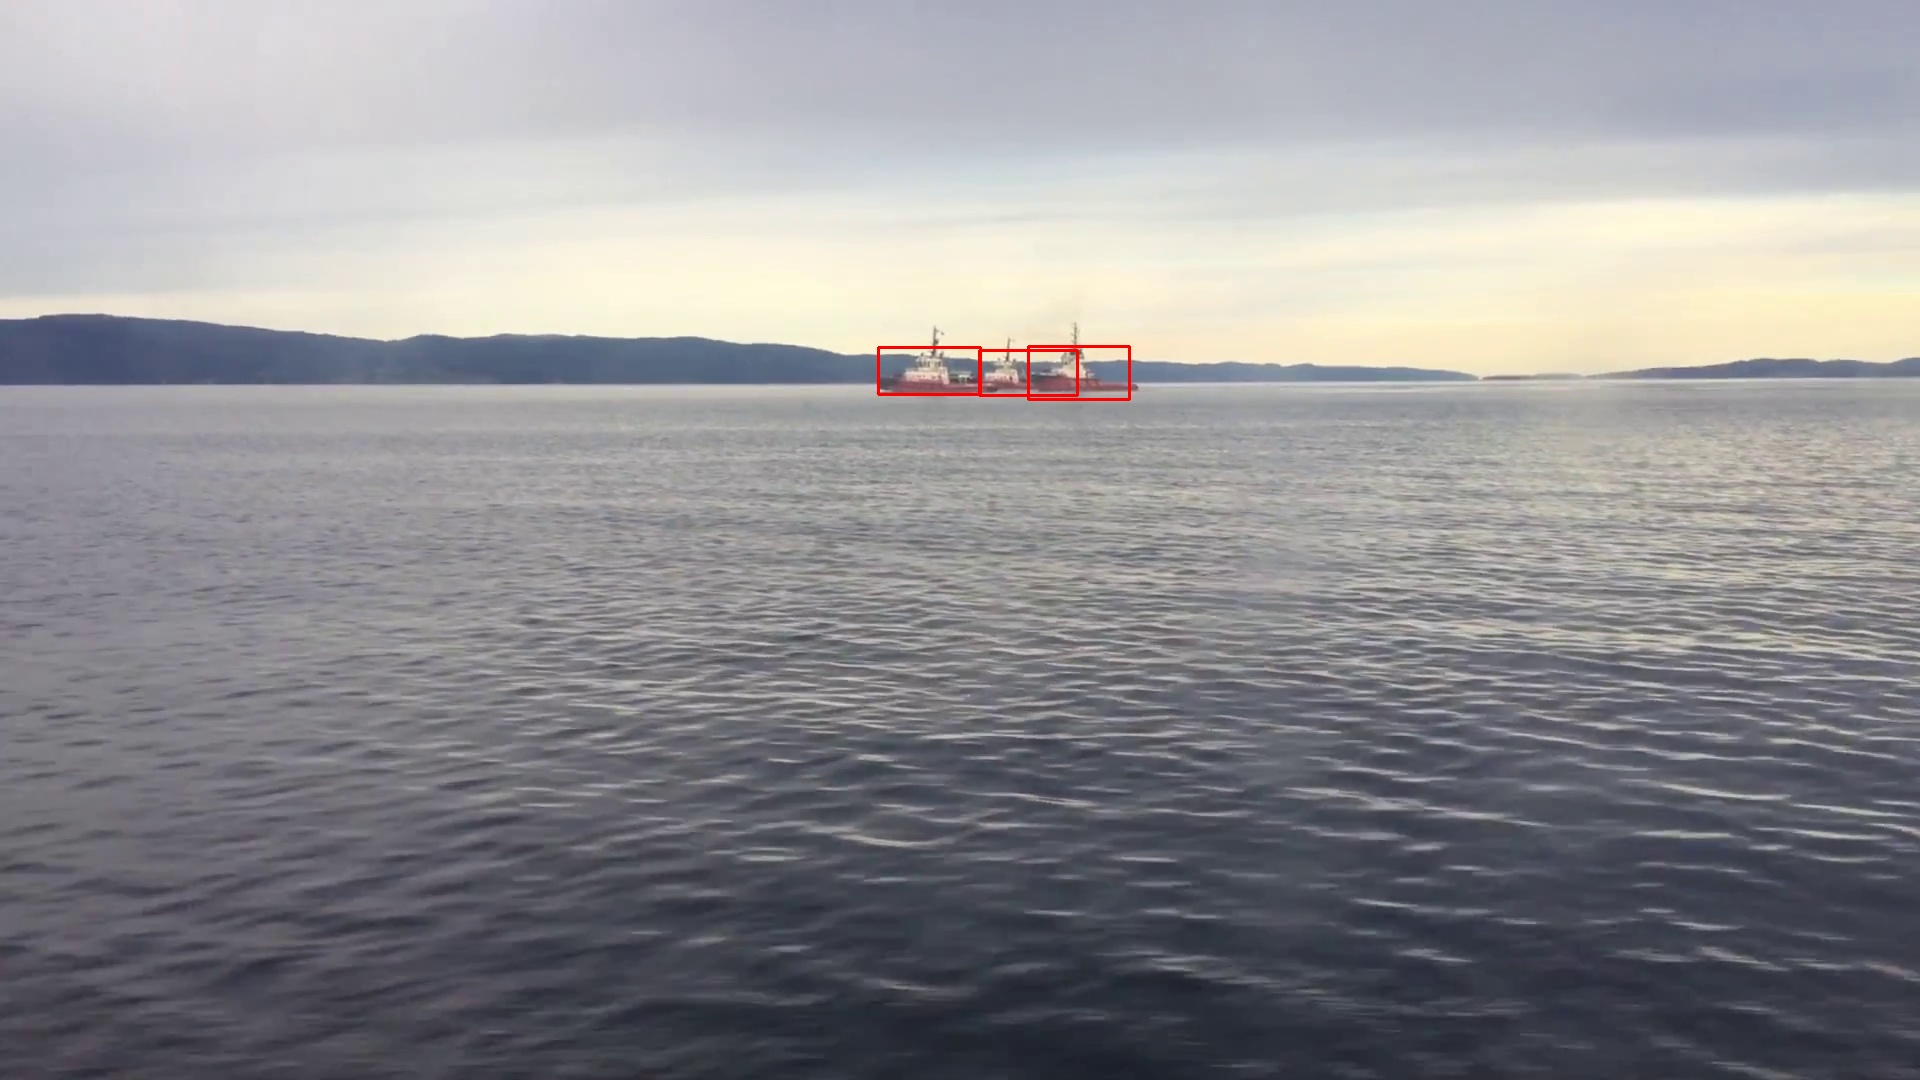
\includegraphics[width=1\linewidth]{results/video/video3/frame20.jpg}
   \caption{Video3}
   \label{fig:video3}
\end{subfigure}
\caption{Frames from video1, video2 and video3}
\label{fig:videos}
\end{figure}

\newpage

In video1 and video2 the boat is detected correctly in every frame. Thus streaks is not an issue in these videos. In both video1 and video2, there is only one boat present. In video3 there are three boats, where one of the boats passes behind another during the video. Yolo1 detects the boats in all frames where the boats are separated, as shown in figure \ref{fig:video3_sep}. When the third boat is behind the second, and beginning to emerge behind it, Yolo1 detects the two boats as one. This is shown in figure \ref{fig:video3_bigboat}. When the third boat is only slightly visible by human assessment, Yolo1 only detects two boats as shown in figure \ref{fig:video3_slightly}. 

\begin{figure}[h!]
\centering
\begin{subfigure}[b]{0.78\textwidth}
   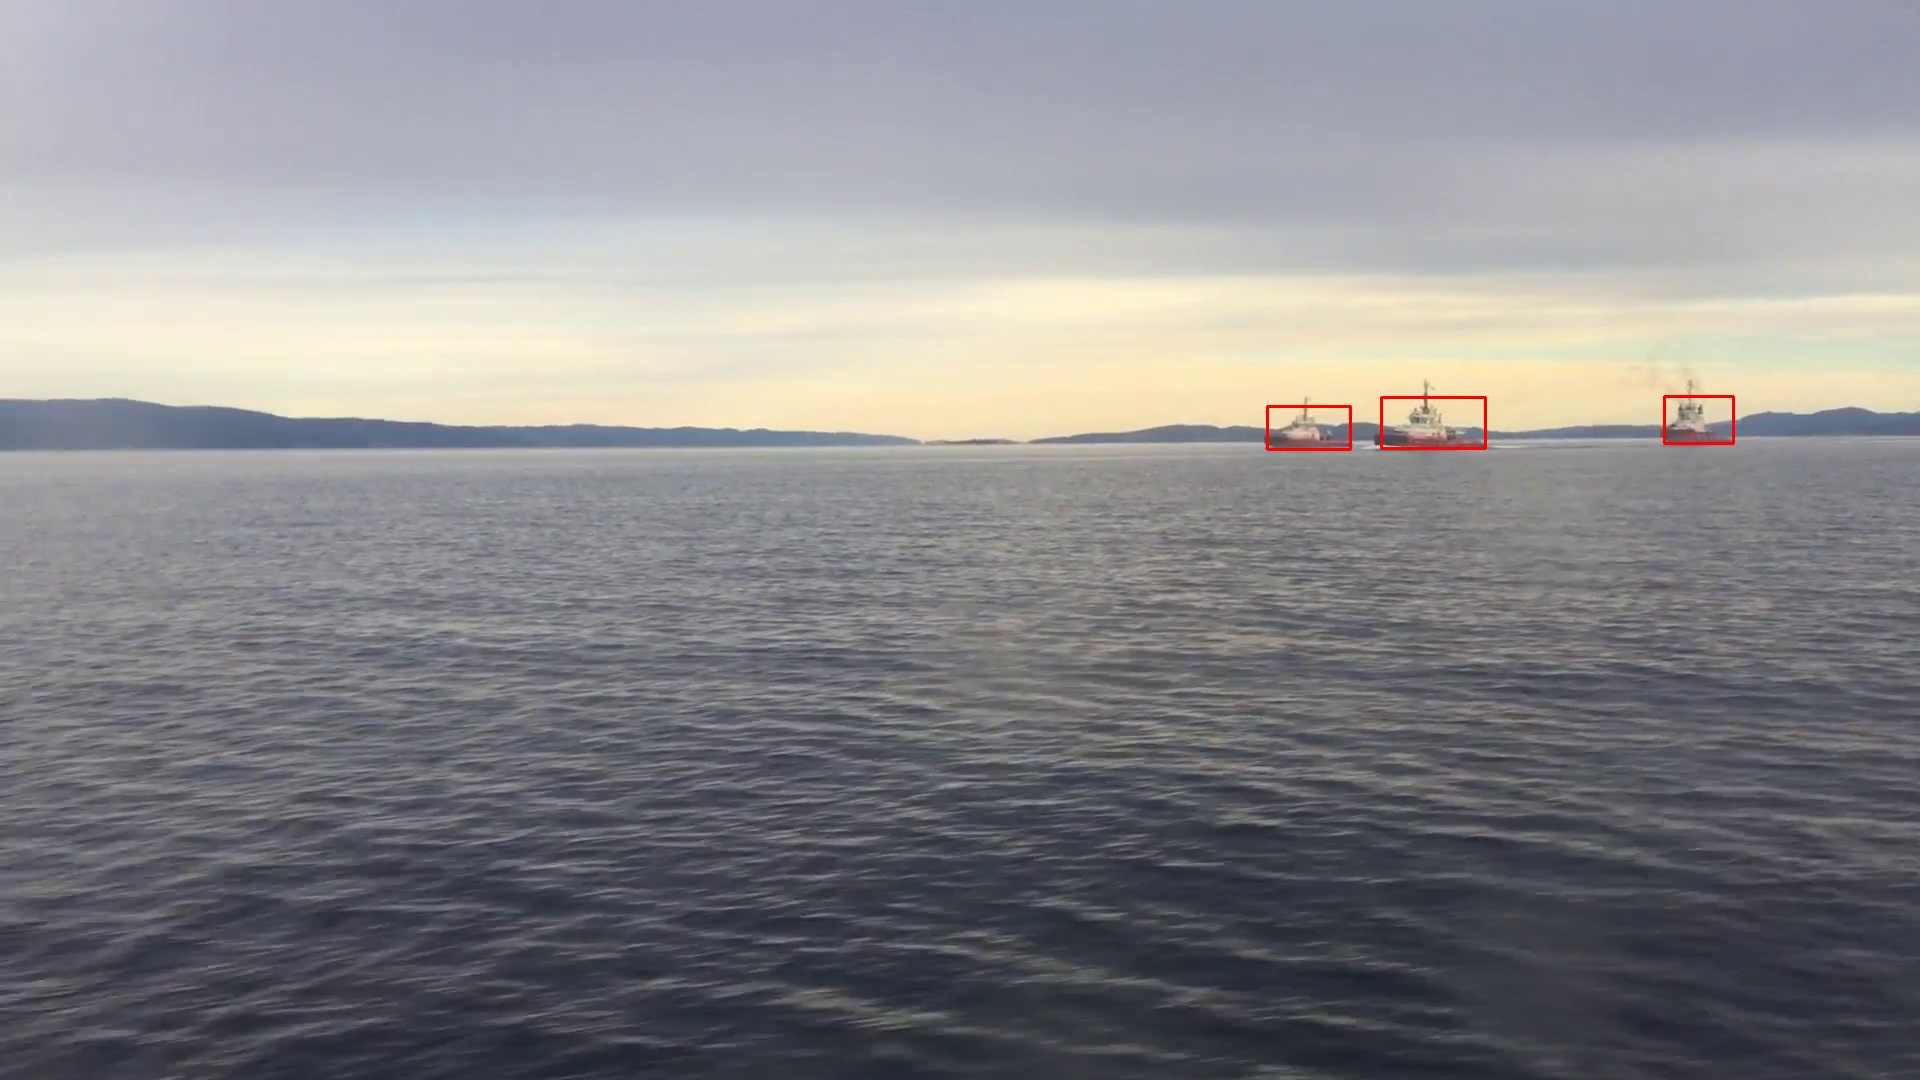
\includegraphics[width=1\linewidth]{results/video/video3/frame677.jpg}
   \caption{Three separated boats}
   \label{fig:video3_sep} 
\end{subfigure}

\begin{subfigure}[b]{0.78\textwidth}
   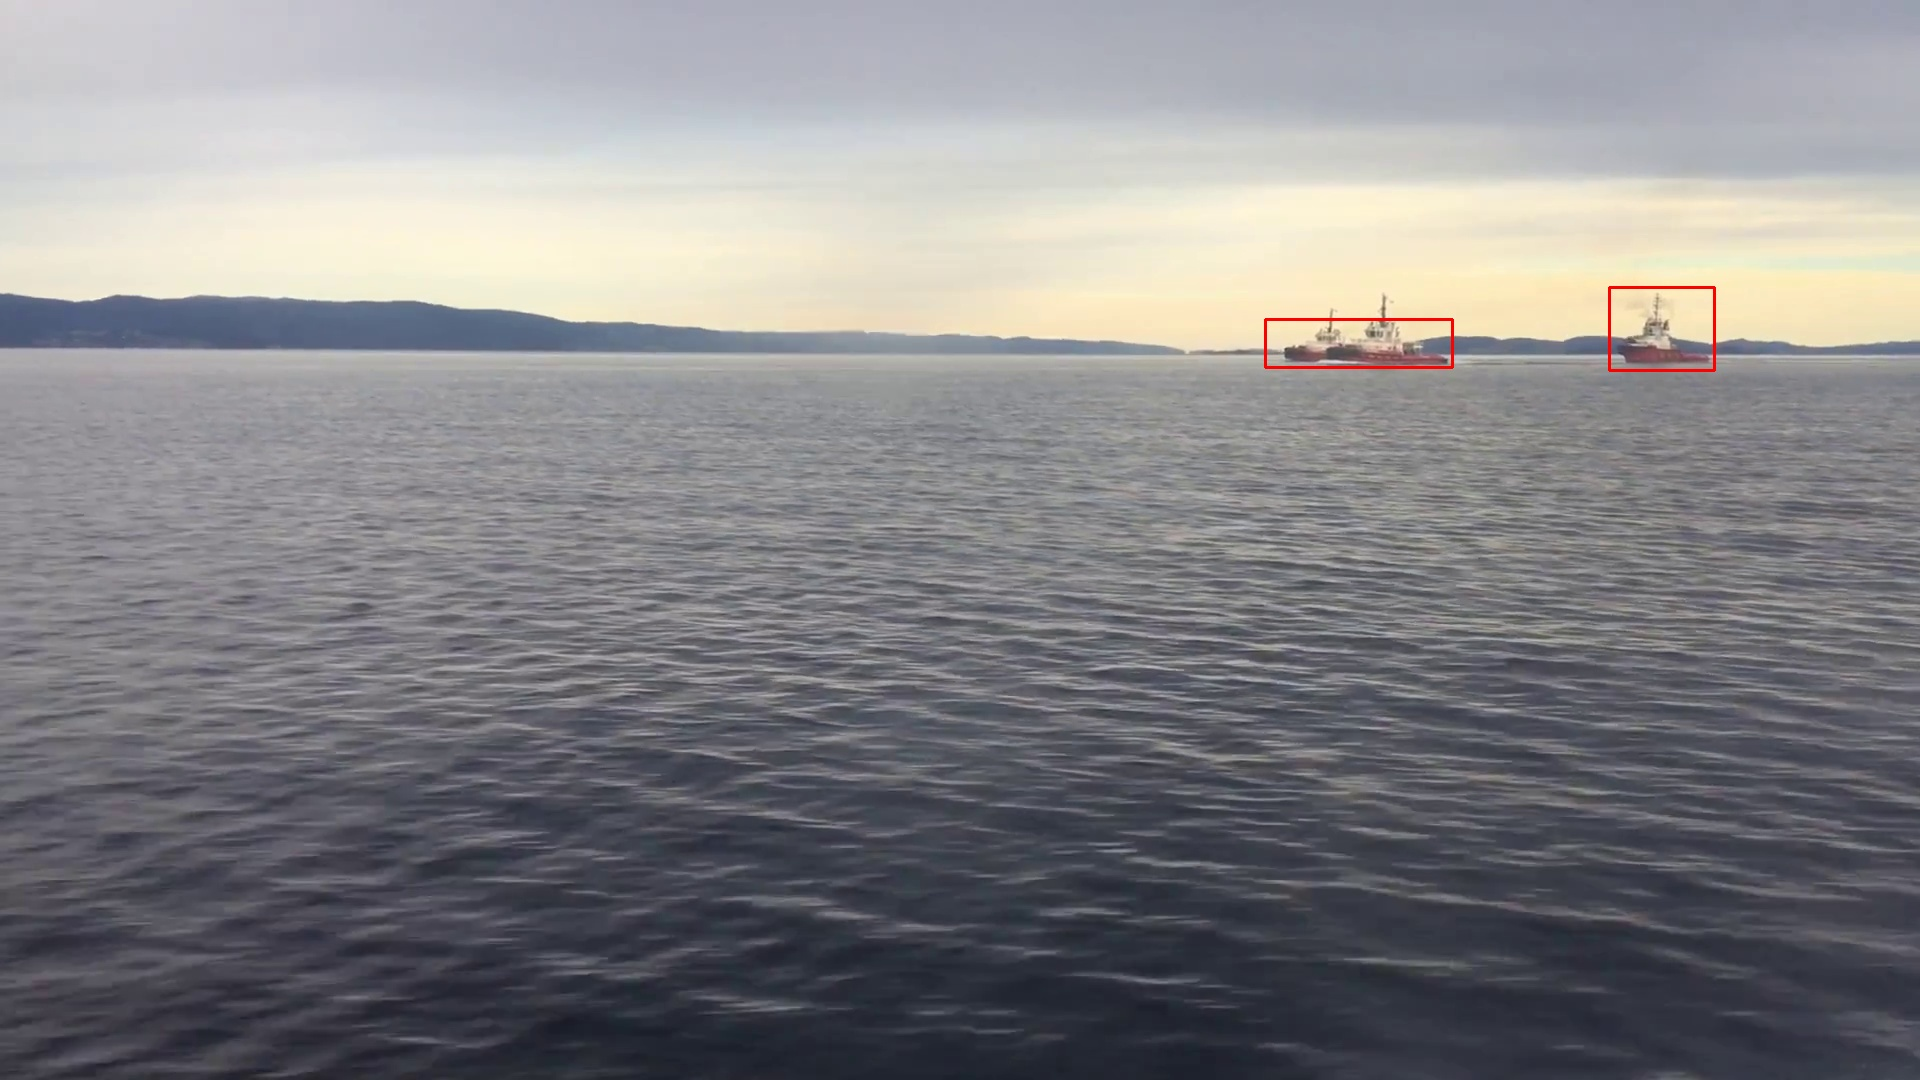
\includegraphics[width=1\linewidth]{results/video/video3/frame479.jpg}
   \caption{Part of third boat clearly visible}
   \label{fig:video3_bigboat}
\end{subfigure}

\begin{subfigure}[b]{0.78\textwidth}
   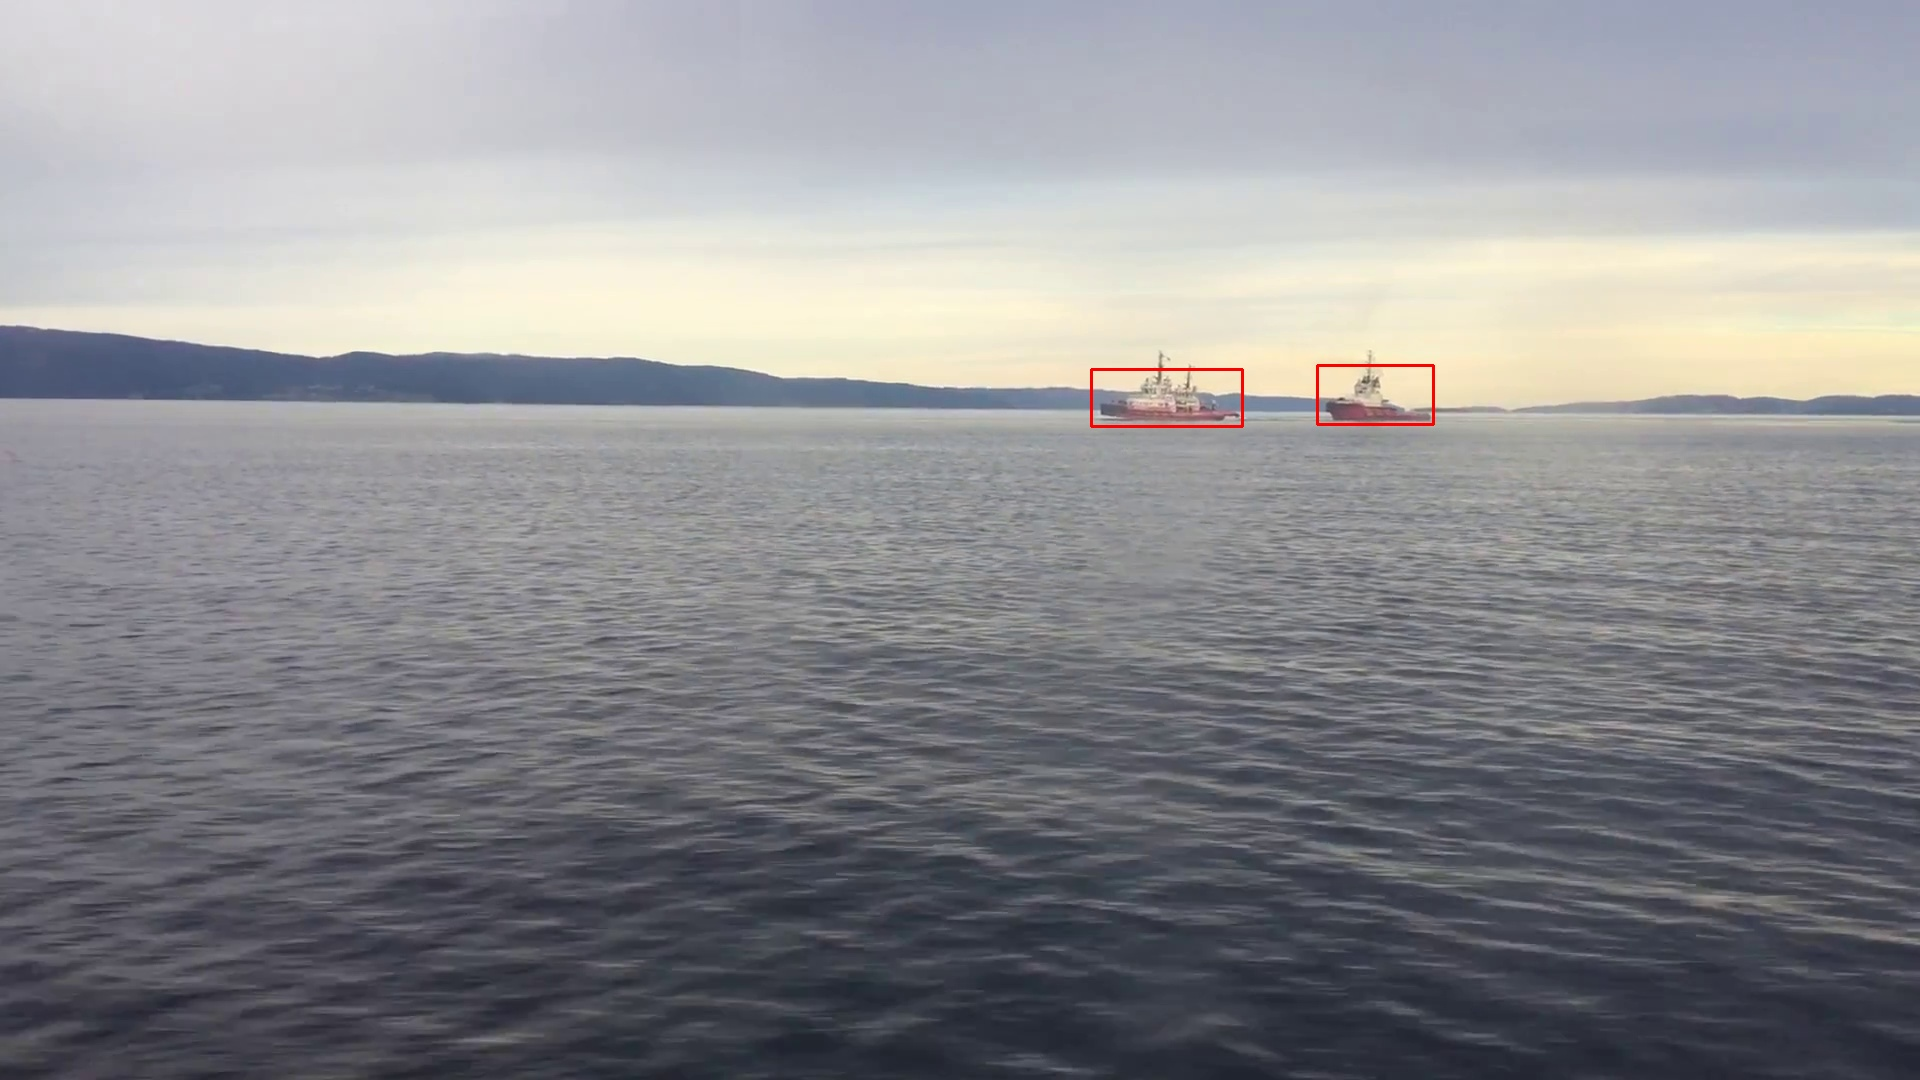
\includegraphics[width=1\linewidth]{results/video/video3/frame208.jpg}
   \caption{Third boat slightly visible}
   \label{fig:video3_slightly}
\end{subfigure}
\caption{Example frames from Video3}
\label{fig:video3}
\end{figure}

\newpage

In video3 all parts of boats are detected as boats, though two boats are classified as one big boat instead of two smaller ones when one is in the shadow of the other. This is a hard problem to solve for an object detector alone, and will be discussed further in chapter \ref{sec:boat_parts}. 


\section{Case Study 4: Video from \citep{Kamsvag2018}}

in \citep{Kamsvag2018} Faster R-CNN was implemented for boat detection. One of the prominent problems encountered in this work was the misclassification of buildings as boats. This was one of the main reasons to train SSD and Yolo on a building class, to see if this could help suppress these detections. Yolo1, Yolo2 and Yolo3 were run on a video used in \citep{Kamsvag2018}, and the results can be found on \url{https://www.youtube.com/watch?v=A_qETwNuFYI}. Example frames from the video are shown in figure \ref{fig:kamsvaag_vid}.

\vspace{3mm}

In this video the images are captured much closer to sea level than the ones used in training, which may have affected the results. Yolo1, Yolo2 and Yolo3 do all have some problems with detecting the boats in the video in every frame, while Yolo1 has the poorest preformance. Yolo3 and Yolo2 have similar results on boat detection, but Yolo3 has more misclassifications of buildings as boats than Yolo2. Yolo3 classifies some of the buildings as buildings, but this does not seem to help suppress the wrong identifications. This will be further discussed in CHAP REF

\begin{figure}[h!]
\centering
\begin{subfigure}[b]{0.6\textwidth}
   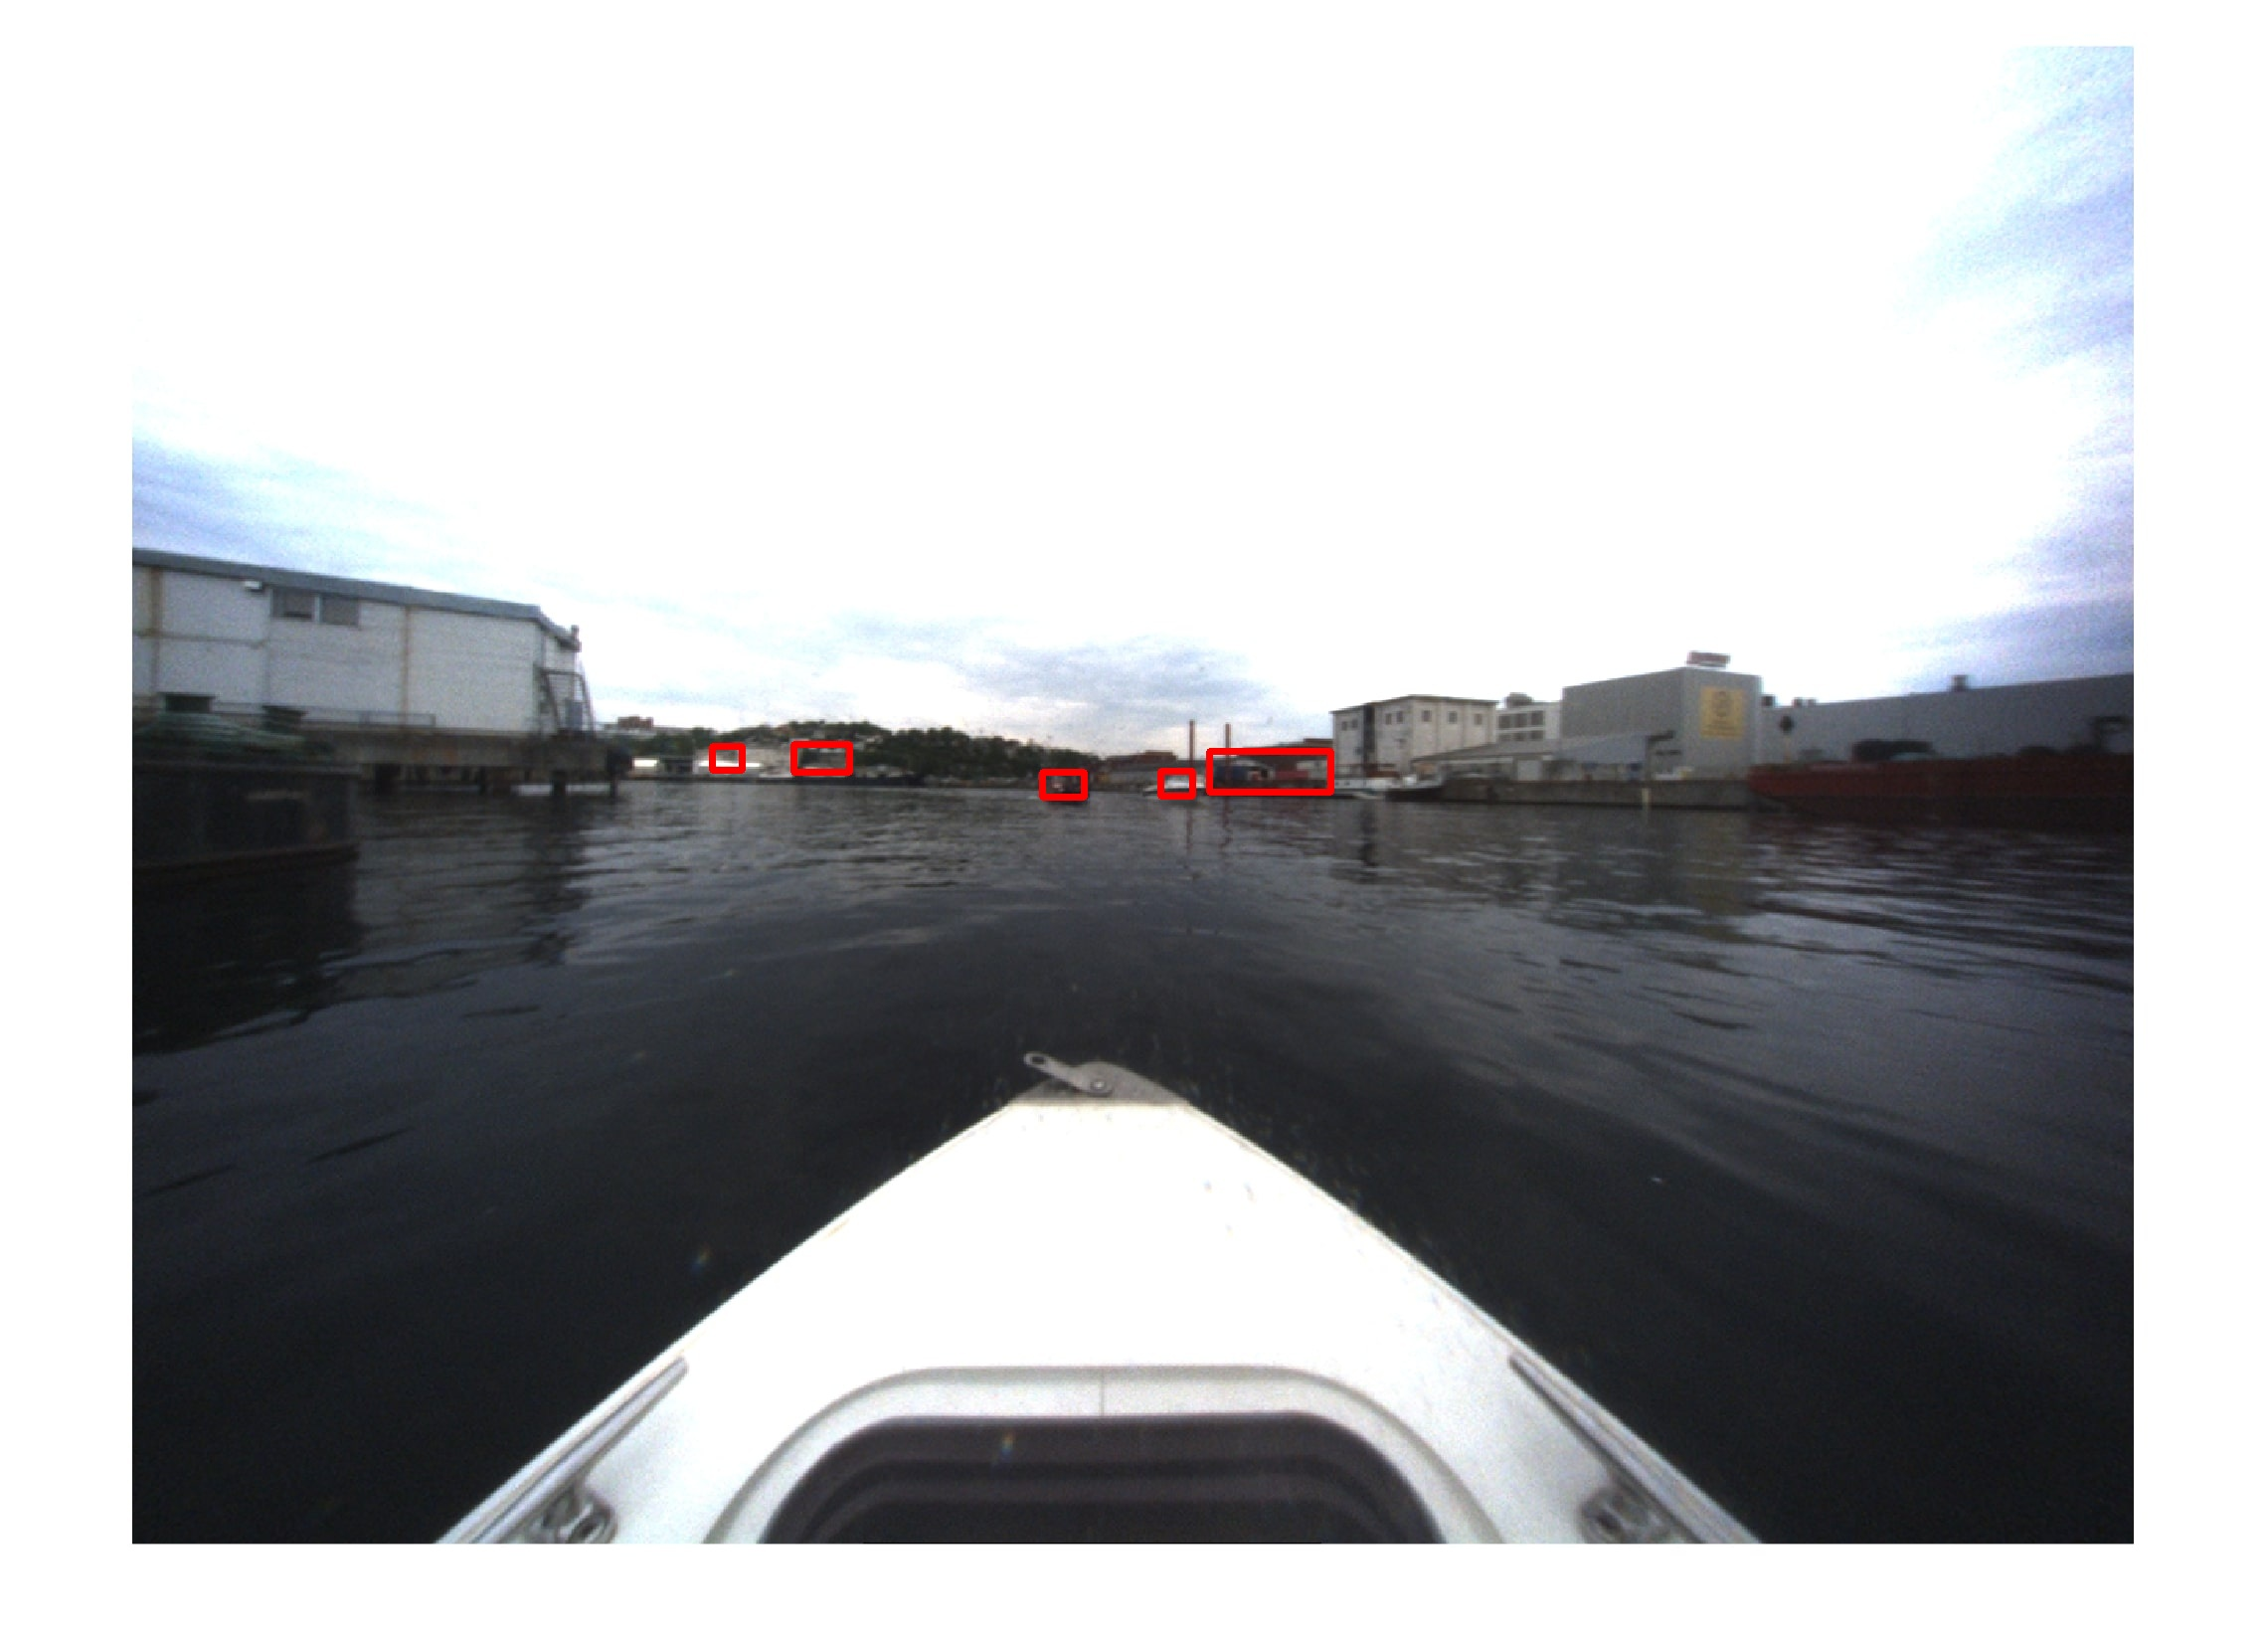
\includegraphics[width=1\linewidth]{results/kamsvag/yolo1_figure_1451.jpg}
   \caption{Yolo1}
   %\label{fig:video3_sep} 
\end{subfigure}

\begin{subfigure}[b]{0.6\textwidth}
   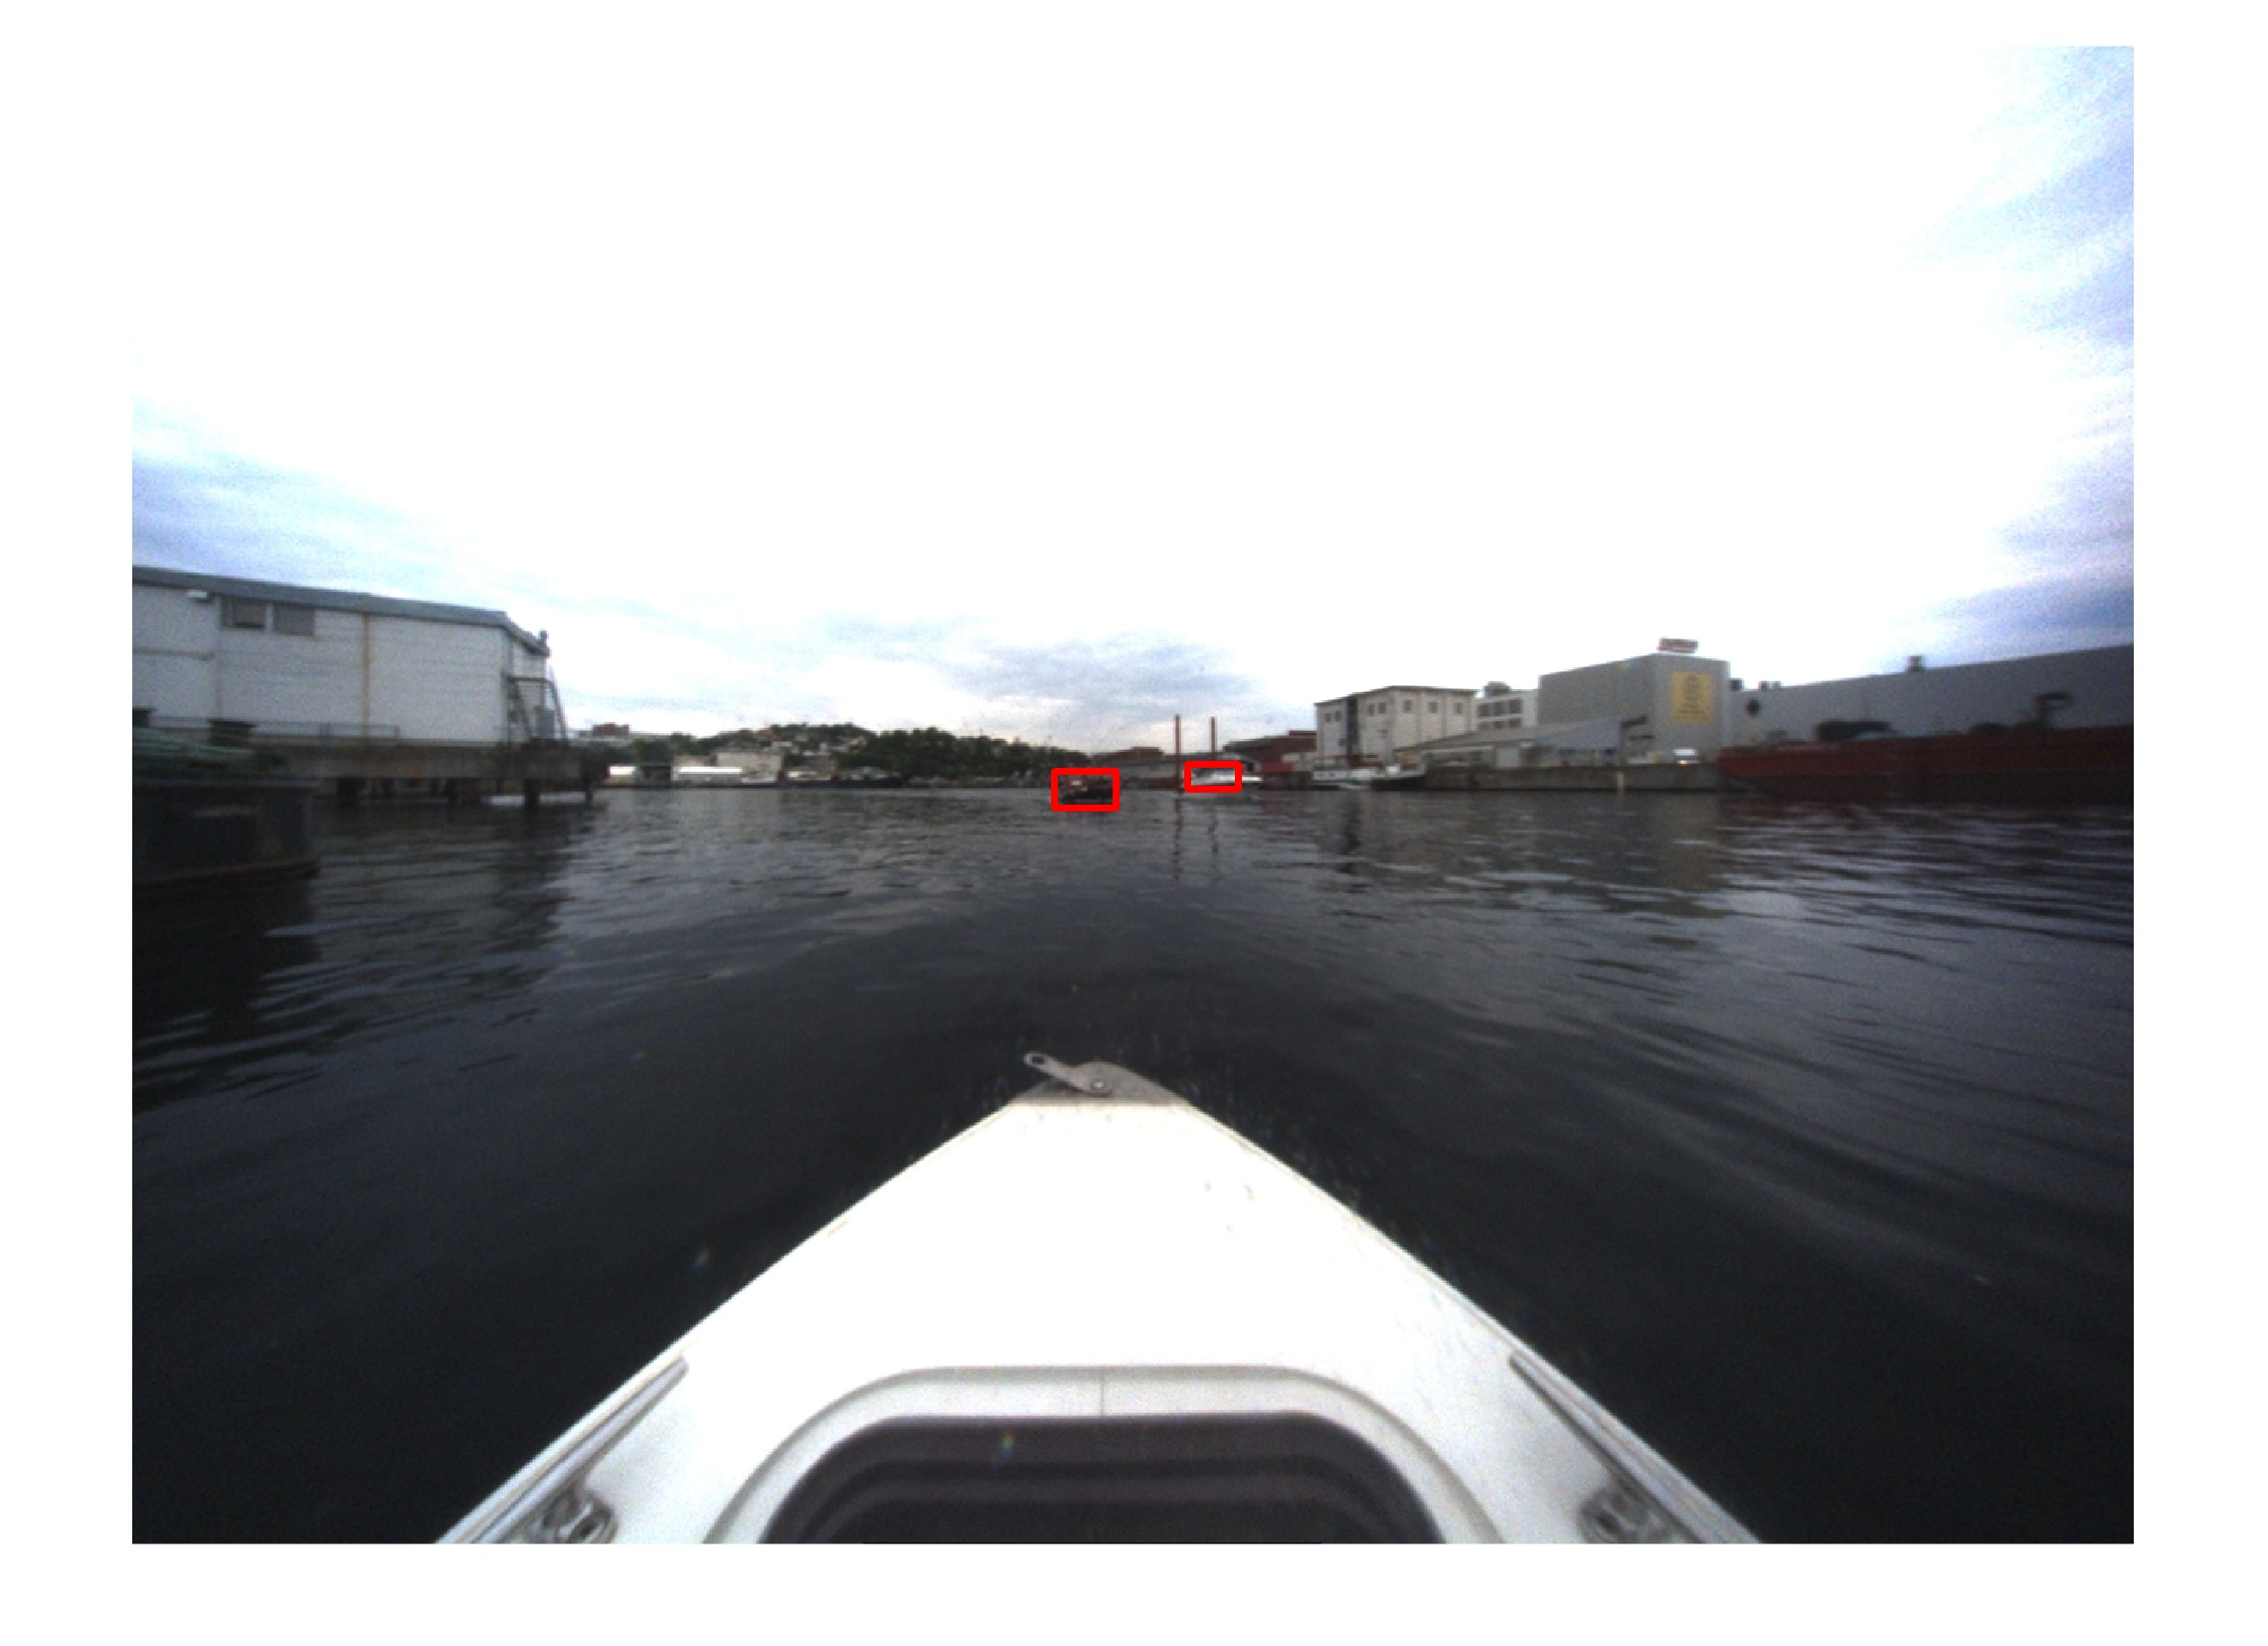
\includegraphics[width=1\linewidth]{results/kamsvag/yolo2_figure_1479.jpg}
   \caption{Yolo2}
   %\label{fig:video3_bigboat}
\end{subfigure}

\begin{subfigure}[b]{0.6\textwidth}
   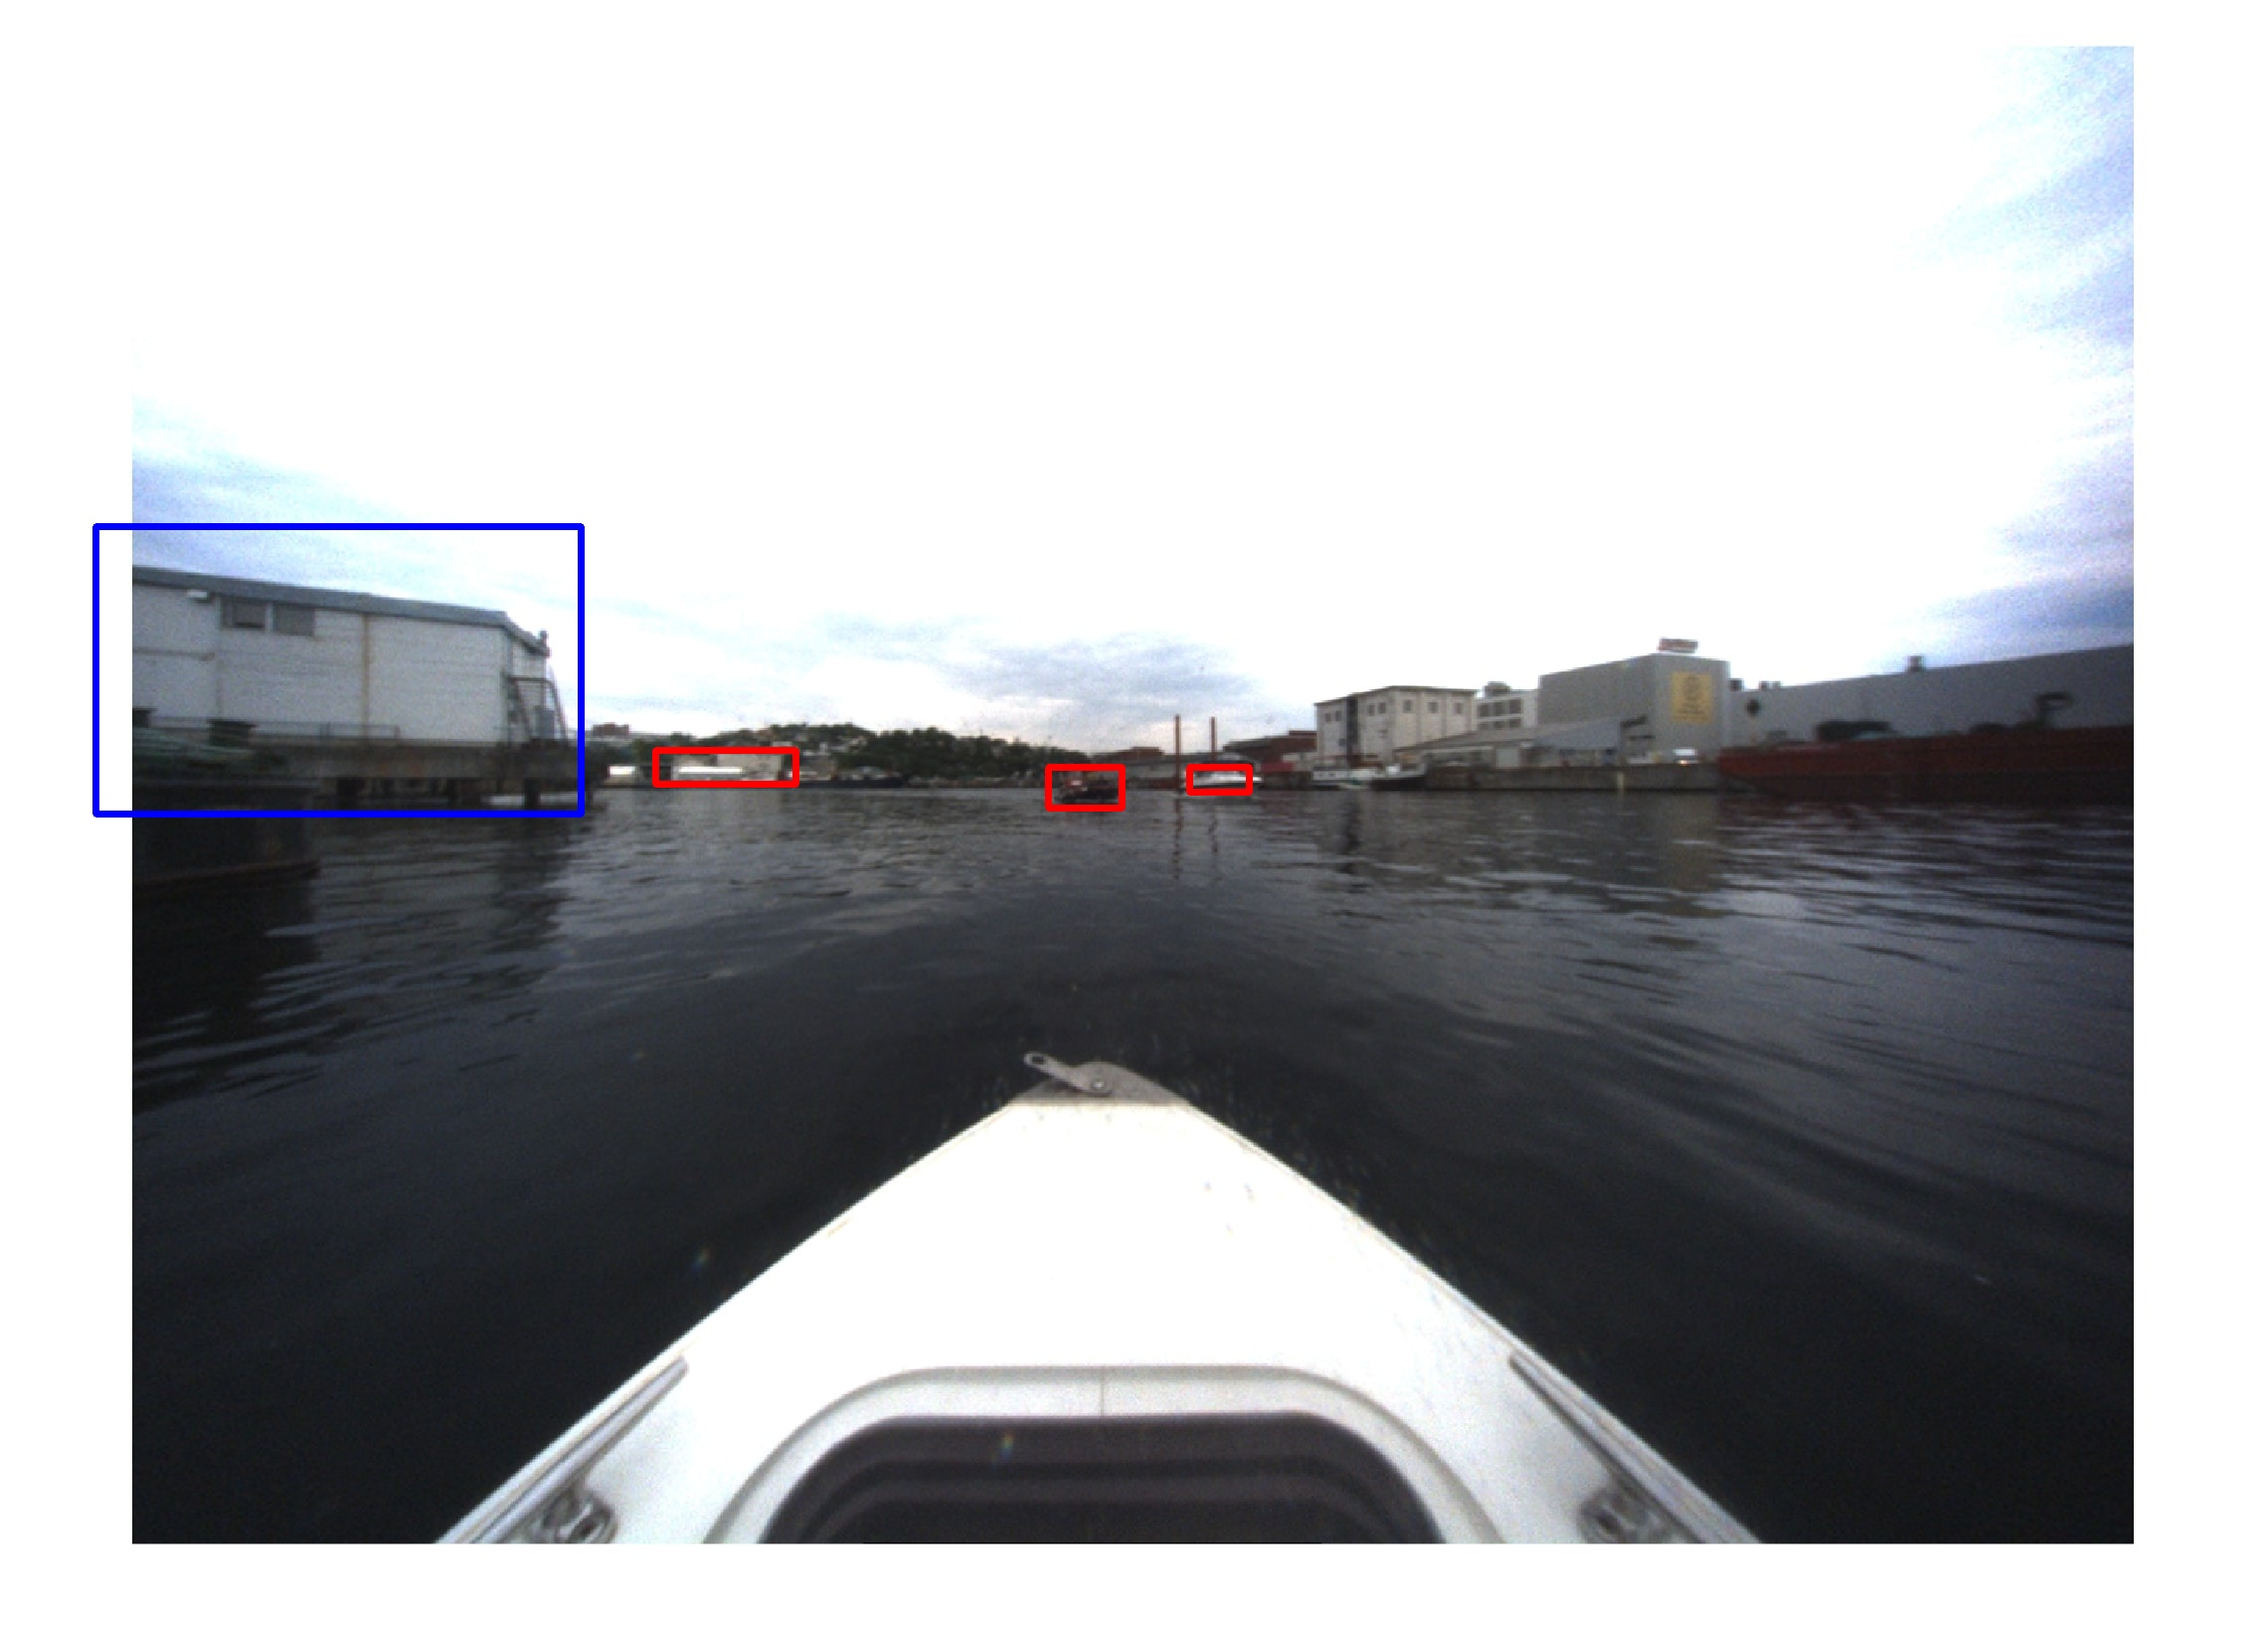
\includegraphics[width=1\linewidth]{results/kamsvag/yolo3_figure_1479.jpg}
   \caption{Yolo3}
   %\label{fig:video3_slightly}
\end{subfigure}
\caption{Example frames from video from \citep{Kamsvag2018}. Red bounding boxes are boat detections, blue boxes are building detections for Yolo3.}
\label{fig:kamsvaag_vid}
\end{figure}


The purpose of training Yolo3 on a building class was for it to be more robust to misclassifications of boats as buildings. In the results shown in CHAP REF, this was not the case. Yolo2, which is not trained on the building class, has fewer detections of buildings as boats than Yolo3. Yolo1, Yolo2 and Yolo3 all gets worse results on this video compared to the results on the rest of the test data. This is not entirely unexpected, since the video from \citep{Kamsvag2018} are different from the training data in several ways. Firstly, the video from \citep{Kamsvag2018} is captured from a small boat close to sea level. This makes the angle between the center of the camera and the center of the boats vastly different compared to the ones in e.g. the \textit{trf} dataset, where the images are taken from the top of a ferry. While the features of the boat does not change much due to the change of angle, the background be different, expecially in coast-near environments. When the pictures are captured from a higher point above sea level the background of the boat will be more uniform, and in some cases consists of only water, while the background can be buildings or land in images taken closer to sea level as in figure \ref{fig:kamsvaag_vid}. While this can be a factor to the weaker boat detections on the video from \citep{Kamsvag2018}, it does not explain why Yolo3 classifies more buildings as boats than Yolo2.

\vspace{3mm}

This being said, it should be noted that the detections of buildings as boats are not consistent over time, and could probably be filtered out in post processing.